\documentclass{article}
% PACKAGES
\usepackage[english]{babel}
\usepackage{graphicx} % Required for inserting images
\usepackage{lmodern}
\usepackage{tcolorbox}
\usepackage{amsmath}
\usepackage{pgfplots}
\usepackage{xcolor}
\usepackage{tikz}
\usepackage{color,soul}
\usepackage{enumerate}
\usepackage{enumitem}
\usepackage{cancel}
\usepackage{hyperref} 
\usepackage{tikzsymbols}
\usepackage{fontawesome5}
\usepackage[export]{adjustbox}
\usepackage{amssymb}
\usepackage{setspace}
\usepackage{sectsty}
\usepackage{booktabs}
\usepackage{subcaption}
\usepackage{tikzsymbols}
\usepackage{textcomp}
\usepackage{marvosym}
\usepackage{parskip}
\usepackage{MnSymbol,wasysym}
\usepackage{multicol}
\usepackage{tikz-cd}
\usepackage{circuitikz}

% newcommand 
\newcommand*\circled[1]{\tikz[baseline=(char.base)]{
            \node[shape=circle,draw,inner sep=2pt] (char) {#1};}}

% COLOURS
\definecolor{Orchid}{RGB}{218, 112, 214}
\definecolor{snow}{rgb}{1.0, 0.98, 0.98}
\definecolor{mordantred19}{rgb}{0.68, 0.05, 0.0}
\definecolor{mistyrose}{rgb}{1.0, 0.89, 0.88}
\definecolor{nadeshikopink}{rgb}{0.96, 0.68, 0.78}
\definecolor{cadmiumgreen}{rgb}{0.0, 0.42, 0.24}
\definecolor{OliveGreen}{RGB}{85, 107, 47}
\definecolor{RoyalPurple}{RGB}{120, 81, 169}
\definecolor{NavyBlue}{RGB}{0, 0, 128}
\definecolor{CornflowerBlue}{RGB}{100, 149, 237}
\definecolor{Cerulean}{RGB}{0, 123, 167}
\definecolor{DarkOrchid}{RGB}{153, 50, 204}
\definecolor{antiquefuchsia}{rgb}{0.57, 0.36, 0.51}
\definecolor{carnationpink}{rgb}{1.0, 0.65, 0.79}
\definecolor{lavenderpurple}{rgb}{0.59, 0.48, 0.71}

\usetikzlibrary{positioning}
\usetikzlibrary{positioning}
\usetikzlibrary{calc,arrows.meta}


\title{MCV4U - Calculus and Vectors}
\author{Made By Kensukeken}
\date{30 January 2024}

\begin{document}
\begin{titlepage}
    \centering
    \begin{tikzpicture}[overlay, remember picture]
        % Background gradient
        \fill[black] (current page.south west) rectangle (current page.north east);
        \fill[left color=violet!80!black, right color=black!40!black] (current page.south west) rectangle (current page.north east);
        % Title
        \node[font=\sffamily\bfseries\Huge, text=white] (title) at (current page.center) {MCV4U - Calculus and Vectors};
        % Author
        \node[below=1cm of title, font=\sffamily\LARGE, text=white] {By Kensukeken};
        % Mathematical symbols and equations
        \node[below=2cm of title, font=\sffamily\Large, text=white] (equation) {$\int_a^b f(x) d x=\lim _{\substack{n \rightarrow \infty \\ \max \Delta x_i \rightarrow 0}} \sum_{i=1}^n f\left(\xi_i\right) \Delta x_i$};
        \node[below=1cm of equation, font=\sffamily\large, text=white] {ISBN: 123-456-789};
        % Colored rectangle
        \fill[lavenderpurple] (title.east) ++(2cm,0) rectangle ++(5cm,-7cm);
    \end{tikzpicture}
\end{titlepage}

\clearpage % New page

\thispagestyle{empty} % No page number

\begin{center}
    
\includegraphics[width=0.5\textwidth]{imgs/OIG4.png} % Adjust the width as needed
\end{center}

\vspace{2cm}

\begin{center}
    \Huge\textbf{Calculus and Vectors}
\end{center}

\vspace{2cm}



\maketitle

\tableofcontents
\newpage



\subsection{Introduction}
\textbf{What is Calculus?}\\
Two simple geometric problems originally led to the development of what is now called calculus. Both problems can be stated in terms of the graph of a function $y=f(x)$.
\begin{itemize}
    \item The problem of tangents: What is the slope of the tangent to the graph of a function at a given point P?
    \item The problem of areas: What is the area under a graph of a function $y=f(x)$ between $x=a$ and $x=b$.
\end{itemize}
    \begin{figure}[ht]
    \centering
    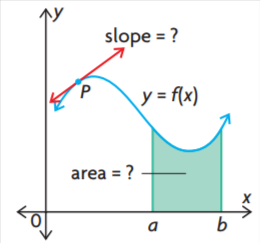
\includegraphics[width=0.35\textwidth]{imgs/Chapter 1 - MCV4U Nelson.png}
    \end{figure}
Isaac Barrow, a professor at the University of Cambridge, recognized the connection between the problem of tangents and the problem of areas. Newton and Gottfried Wilhelm von Leibniz independently solved these problems using differentiation and integration, a major advance in mathematics. This discovery led to the creation of calculus, a powerful branch of mathematics used in applied mathematics, science, engineering, and economics. The study of calculus begins with the meaning of a tangent, rate of change, limits, and the derivative of a function.
\newpage

\subsection*{Radical Expressions: Rationalizing Denominators}
In calculus, rationalizing the denominator of radical expressions involves simplifying expressions with radicals in the denominator. This process simplifies numbers into integers, making dividing by an integer more preferable than dividing by a radical number. \\ 

\subsection*{\textcolor{blue}{Selecting a strategy to rationalize the denominator}}
\begin{align*}
&\text{Simplify the radical expression } \frac{5}{2 \sqrt{6}+3} \text{ by rationalizing the denominator.} \\
&\text{Solution} \\
&\frac{5}{2 \sqrt{6}+3} = \frac{5}{2 \sqrt{6}+3} \times \frac{2 \sqrt{6}-3}{2 \sqrt{6}-3} \quad \text{(The conjugate $2 \sqrt{6}+\sqrt{3}$ is $2 \sqrt{6}-\sqrt{3}$)} \\
&= \frac{5(2 \sqrt{6}-3)}{4 \sqrt{36}-9} \\
&= \frac{5(2 \sqrt{6}-3)}{24-9} \\
&= \frac{5(2 \sqrt{6}-3)}{15} \\
&\text{(Divide by the common factor of 5)} \\
&= \frac{2 \sqrt{6}-3}{3}
\end{align*}
\\\\
When the denominator of a radical fraction is a two-term expression, you can rationalize the denominator by multiplying by the \textbf{\textcolor{blue}{conjugate}}. \\ \\
An expression such as $\sqrt{a}+\sqrt{b}$ has $\sqrt{a}-\sqrt{b}$ the conjugate.\\\\
Why are conjugates important? Recall that the linear terms are eliminated when
expanding a difference of squares. For example,
\begin{align*}
    (a-b)(a+b)&=a^2+ab-ab-b^2 \\
    &=a^2-b^2
\end{align*}
If a and b were radicals, squaring them would rationalize them.
\begin{align*}
\text{Consider this product:}\quad
    &(\sqrt{x}-\sqrt{y})(\sqrt{x}+\sqrt{y}), \; x, \text{y rational} \\ &=(\sqrt{x})^2+\sqrt{xy}-\sqrt{xy}-(\sqrt{x})^2 \\
    &=x-y \quad \textbf{Notice that the result is rational!}
\end{align*}

\newpage
\section{Unit 1 - Limits}
\subsection{Evaluating Limits Graphically}
Imagine someone is standing 10 metres from a wall. We tell that person to move halfway to the wall. We then them to again move halfway to the wall. We then tell them to again move halfway to the wall, and we continue to do this. Theoretically, the person will never reach the wall. However, we can say that as the number of trials moves to infinity, the limit of where the person is standing will be the wall.

Of course, the person will never each the wall(theoretically), but we could still refer to the wall as the limit.

Another way to think about limits is to think about sequnces.

Consider the sequence $f(n)$ where n is a positive integer referring to the ordinal position of the term in the sequence and $f(n)$ is the value of that term.
$$1,\frac{1}{2},\frac{1}{4},\frac{1}{8},\frac{1}{16}, \cdots $$
The values are getting closer and closer to 0. We know that the values will never reach 0, but they will get infinitely close to 0. We can say that the limit of the sequence as the number of terms goes to infinity is 0.

$$\lim_{n \to \infty} f(n)=0$$
In mathematics, a limit is the value that a function(or sequence) "approaches" as the input (or index) "approaches" some value. Limits are essential to calculus(and mathematical analysis in general) and are used to define continuity, derivatives, and integrals.When dealing with functions, we can let the x-value inputted to the function grow closer and closer to some set value. We then watch the pattern of y-values to see if there is a set y-value that we grow infinitely close to. If there is such a value, we say that that is the value of the limit

\subsubsection{Example:}
Suppose that we wish to determine $\lim_{x \to 3} (-x^2+6x-5 )$. We can draw the graph of $y=-x^2+6x-5$:

\begin{minipage}{0.6\textwidth}
    \begin{align*}
        \lim_{x \to 3^-} f(x) &= 4 \\
        \lim_{x \to 3^+} f(x) &= 4 \\
        \lim_{x \to 3} f(x) &= 4
    \end{align*}
\end{minipage}%
\vspace{1em}%
\begin{minipage}{0.6\textwidth}
    The graph of $y=-x^2+6x-5$:
    \begin{center}
        \begin{tikzpicture}[scale=0.2]
            % Axis
            \draw[->] (-1,0) -- (7,0) node[right] {$x$};
            \draw[->] (0,-7) -- (0,6) node[above] {$y$};
          
            % Function plot
            \draw[domain=0:6, smooth, variable=\x, blue] plot ({\x}, {-\x^2 + 6*\x - 5});
            \fill[red] (3, 4) circle (3pt) node[above right] {(3,4)};

          
            % Labels
            \node[below] at (6,0) {$6$};
            \node[left] at (0,-5) {$-5$};
        \end{tikzpicture}
    \end{center}
\end{minipage}
When determining whether the limit as x approaches a particular value of a function exists, we compare the two one-sided limits and see if they are the same. If they are, then the limit exists, and is equal to that common value.
\\ 
\begin{tcolorbox}[colback=Orchid!5!white,colframe=cadmiumgreen!75!white,coltitle=white,]
If $\lim _{x \rightarrow a^{-}} f(x)=b$ and if $\lim _{x \rightarrow a^{+}} f(x)=b$ then $\lim _{x \rightarrow a} f(x)=b$
However, if $\lim _{x \rightarrow a^{-}} f(x)$ exists and if $\lim _{x \rightarrow a^{+}} f(x)$ exists but $\lim _{x \rightarrow a^{-}} f(x) \neq \lim _{x \rightarrow a^{+}} f(x)$, then $\lim _{x \rightarrow a} f(x)$ does not exist. \\ \\ 
\end{tcolorbox}

Note that in the last example, we expressed that limits were described as being equal to $\infty$ and to $-\infty$. Technically, nothing can be equal to $\infty$ or $-\infty$, so one could immediately conclude that $\lim_{x \to 4}\left( \frac{x+1}{x-4}\right)$ does not exist, as soon as one of the one-sided limits is equal to $\infty$ or $-\infty$. However, in this course, we will allow one-sided limits to be expressed as $\infty$ or $-\infty$. This will include limits as $x$ approaches $\infty$ or $-\infty$, which can only be approached from one direction. 

However, if we are seeking the limit of a function as $x$ approaches a real number (a two-sided limit), and if one of the one-sided limits is equal to $\infty$ or $-\infty$, then we will state that the limit of the function as $x$ approaches the real number does not exist.
\\
\subsubsection*{Limits that can only be approached from one side:}
Sometimes, we will come across a limit that can only be approached from the left or from the right. The most common type of limit of this form is when we seek to find the limit of a function as $x$ approaches $\infty$ or as $x$ approaches $-\infty$.

If we want to evaluate the limit of a function as $x$ approaches $-\infty$, we can only approach it from the right because we can’t be to the left of $-\infty$. Similarly, if we want to evaluate the limit of a function as $x$ approaches $\infty$, we can only approach it from the left because we can’t be to the right of $\infty$.

\begin{table}[h]
    \centering
    \begin{tabular}{|c|l|}
    \hline
    Expression & Explanation \\
    \hline
    $\frac{0}{0}$ & Indeterminate: maybe the limit and maybe it doesn't. Do more work! \\
    \hline
    $\frac{\text{Non-Zero}}{0}$ & The limit does not exist. You're done working. \\
    \hline 
    $\frac{\text{Anything}}{\text{Non-Zero}}$ & That's the answer :) \\
    \hline
    \end{tabular}
    \caption{Limit Evaluation Cases}
    \label{tab:limits}
\end{table}

\newpage

\subsection{Evaluating Limits Algebraically}
Assume that we are trying to evaluate $\lim_{x \to c}f(x), c \in \mathrm{R}$\\

We often don't use a graphing approach to evaluate a limit. Rather, we can use an algebraic approach if we remember the following steps. \\
\begin{enumerate}
    \item  \text{\hl{If the curve is continuous at $\mathrm{x}=\mathrm{c}$}}, then we can simply evaluate $\mathrm{f}(\mathrm{c})$. In other words, $\lim _{x \rightarrow c} f(x)=f(c)$ \\
    \begin{itemize}
        \item This happened in the first example in the powerpoint about evaluating limits graphically. When we were seeking to evaluate $\lim _{x \rightarrow 3}\left(-x^2+6 x-5\right)$, we could have recognized that this was a continuous function at $x=3$ and simply plugged in an $x$-value of 3 .
   \end{itemize}
\item \hl{However, sometimes direct substitution leads to a result of $0 / 0$.} Obviously, this result is undefined. However, the limit may still exist because there may be a hole at $\mathrm{x}=\mathrm{c}$ in an otherwise continuous curve.
\begin{itemize}
    \item This is what happened in some of our examples in the powerpoint on graphically evaluating limits. For example, in the example where we sought $\lim _{x \rightarrow-2}\left(\frac{x^2+3 x+2}{x+2}\right)$, there was a hole and the value of the limit equaled the $y$-coordinate of the location of the hole.
\end{itemize} 
When we get the indeterminate form of $0 / 0$, we can try the following:
\begin{tcolorbox}[colback=Orchid!5!white,colframe=Orchid!75!white,coltitle=white,]
\begin{enumerate}[label=(\roman*)]
    \item Factor numerator and denominator, and the offending factor may cancel out of both
    \item Rationalize the numerator and/or denominator and see if this leads you to be able to directly substitute
    \item Simplify the function prior to substituting to see if that allows you to directly substitute iv. Introduce a new factor that allows the numerator and/or denominator to become a difference or sum of nth powers, which then creates the offending factor which can then be canceled from both numerator and denominator (you may wish to introduce a new variable to do this)
\end{enumerate}
\end{tcolorbox}
\end{enumerate}
\newpage

\subsubsection{Examples where direct substitution leads to the correct answer}
\textbf{Examples}\\
1. Evaluate $\lim_{x \to 5}x^2+2x-3$
\begin{align*}
\lim_{x \to 5}x^2+2x-3 &= \text{Plug } x=5 \\ 
    &= (5)^2+2(5)-3 \\
    &= \boxed{32} \quad \text{That's the answer } 
\end{align*}
2. Evaluate $\lim_{x \to 3}\frac{\sqrt{x-1}-\sqrt{x+1}}{\sqrt{x-3}-\sqrt{x+3}}$\\
\begin{align*}
    &=\frac{\sqrt{3-1}-\sqrt{3+1}}{\sqrt{3-3}-\sqrt{3+3}}\\
    &=\frac{\sqrt{2}-\sqrt{4}}{\sqrt{0}-\sqrt{6}}\\
    &=\frac{\sqrt{2}-2}{-\sqrt{6}}
\end{align*}

2a)  Examples where Direct Substitution Leads to 0/0 But you can then factor, cross out, and then sub in\\\\
3. Evaluate $\lim_{h \to 0}\frac{(2+h)^3-8}{h}$
\begin{align*}
    &\text{Recall}: a^3-b^3 = (a-b)(a^2+ab+b^2)\\
    &=\lim_{h\to 0}\frac{\cancel{8}+12h^+6h^2+h^2\cancel{-8}}{h}\\
    &=\lim_{h\to 0}\frac{h^3+6h^2+12}{h}\\
    &=\lim_{h \to 0}\frac{\cancel{h}(h^2+6h+12)}{\cancel{h}}\\
    &= (0)^2+6(0)+12\\
    &=12
\end{align*}
4. Evaluate $\lim_{x \to 25}\frac{x-25}{\sqrt{x}-5}$
\begin{align*}
    &=\lim_{x \to 25}\frac{x-25}{\sqrt{x}-5} \times \frac{(\sqrt{x})^2-(5)^2}{\sqrt{x}-5}\\
    &=\lim_{x \to 25}\frac{\cancel{(\sqrt{x}-5)}(\sqrt{x}+5)}{\cancel{(\sqrt{x}-5)}}\\
    &=\sqrt{25}+5\\
    &=10
\end{align*}
\subsubsection{Difference of nth Powers Factoring}

The formula for factoring the difference of nth powers is:

\[
a^n - b^n = (a - b)(a^{n-1} + a^{n-2}b + a^{n-3}ba^2 + \cdots + ab^{n-2} + b^{n-1})
\]

Examples of the difference of nth powers factored from \(a^2 - b^2\) to \(a^{10} - b^{10}\) using the formula:

\begin{enumerate}
    \item \(a^2 - b^2\):
    \[
    a^2 - b^2 = (a - b)(a + b)
    \]
    
    \item \(a^3 - b^3\):
    \[
    a^3 - b^3 = (a - b)(a^2 + ab + b^2)
    \]
    
    \item \(a^4 - b^4\):
    \[
    a^4 - b^4 = (a - b)(a^3 + a^2b + ab^2 + b^3)
    \]
    
    \item \(a^5 - b^5\):
    \[
    a^5 - b^5 = (a - b)(a^4 + a^3b + a^2b^2 + ab^3 + b^4)
    \]
    
    \item \(a^6 - b^6\):
    \[
    a^6 - b^6 = (a - b)(a^5 + a^4b + a^3b^2 + a^2b^3 + ab^4 + b^5)
    \]
    
    \item \(a^7 - b^7\):
    \[
    a^7 - b^7 = (a - b)(a^6 + a^5b + a^4b^2 + a^3b^3 + a^2b^4 + ab^5 + b^6)
    \]
    
    \item \(a^8 - b^8\):
    \[
    a^8 - b^8 = (a - b)(a^7 + a^6b + a^5b^2 + a^4b^3 + a^3b^4 + a^2b^5 + ab^6 + b^7)
    \]
    
    \item \(a^9 - b^9\):
    \[
    a^9 - b^9 = (a - b)(a^8 + a^7b + a^6b^2 + a^5b^3 + a^4b^4 + a^3b^5 + a^2b^6 + ab^7 + b^8)
    \]
    
    \item \(a^{10} - b^{10}\):
    \[
    a^{10} - b^{10} = (a - b)(a^9 + a^8b + a^7b^2 + a^6b^3 + a^5b^4 + a^4b^5 + a^3b^6 + a^2b^7 + ab^8 + b^9)
    \]
\end{enumerate}

These examples demonstrate the application of the difference of nth powers factoring formula for various powers from 2 to 10.

\subsection*{Sum of nth Powers Factoring (for odd n)}

If \( n \) is an odd positive integer, the sum of nth powers can be factored as follows:

\[
a^n + b^n = (a + b)(a^{n-1} - a^{n-2}b + a^{n-3}b^2 - \cdots - ab^{n-2} + b^{n-1})
\]

This formula works only when \( n \) is an odd positive integer.

\subsection*{Examples}

Let's consider the following examples:

\begin{enumerate}
    \item For \( n = 2 \):
    \[
    a^2 + b^2 \quad \text{(This formula doesn't apply)}
    \]
    
    \item For \( n = 3 \):
    \[
    a^3 + b^3 = (a + b)(a^2 - ab + b^2)
    \]
    
    \item For \( n = 4 \):
    \[
    a^4 + b^4 \quad \text{(This formula doesn't apply)}
    \]
    
    \item For \( n = 5 \):
    \[
    a^5 + b^5 = (a + b)(a^4 - a^3b + a^2b^2 - ab^3 + b^4)
    \]
    
    \item For \( n = 6 \):
    \[
    a^6 + b^6 \quad \text{(This formula doesn't apply)}
    \]
    
    \item For \( n = 7 \):
    \[
    a^7 + b^7 = (a + b)(a^6 - a^5b + a^4b^2 - a^3b^3 + a^2b^4 - ab^5 + b^6)
    \]
    
    \item For \( n = 8 \):
    \[
    a^8 + b^8 \quad \text{(This formula doesn't apply)}
    \]
    
    \item For \( n = 9 \):
    \[
    a^9 + b^9 = (a + b)(a^8 - a^7b + a^6b^2 - a^5b^3 + a^4b^4 - a^3b^5 + a^2b^6 - ab^7 + b^8)
    \]
    
    \item For \( n = 10 \):
    \[
    a^{10} + b^{10} \quad \text{(This formula doesn't apply)}
    \]
\end{enumerate}

These examples demonstrate the application of the formula for factoring the sum of nth powers when \( n \) is an odd positive integer.

\subsection*{Sum of nth powers factoring is really just an extension of difference of nth powers factoring.}
For example, consider $a^5+b^5$

$$
\begin{aligned}
& a^5+b^5 \\
& =a^5-(-b)^5 \\
& =[a-(-b)]\left[a^4+a^3(-b)+a^2(-b)^2+a(-b)^3+(-b)^4\right] \\
& =[a+b]\left[a^4+\left(-a^3 b\right)+a^2 b^2+\left(-a b^3\right)+b^4\right] \\
& =(a+b)\left(a^4-a^3 b+a^2 b^2-a b^3+b^4\right)
\end{aligned}
$$ 
\subsection*{Check Your Understanding:}
\begin{enumerate}
    \item Evaluate $\lim_{x \to 3}\frac{2x^4-162}{-x^5+243}$
    \item Evaluate $\lim_{x \to -2}\frac{x^7+128}{10x+20}$ 
\end{enumerate}
Feel free to download \href{https://github.com/Kensukeken/MCV4U-Calculus-and-Vectors-Notes/blob/main/Lessons%20in%20Power%20Point%20Form/Unit%201/chap%201.010.evaluating%20limits%20graphically.pptx}{chap 1.020.evaluating limits algebraically.pptx} to check the solutions :) 

 2b)  Examples where direct substitution leads to 0/0 but we can rationalize the numerator and/or denominator, then perhaps factor, then cross out then substitute\\

 1. Evaluate $\lim_{h\to 0}\frac{\sqrt{16+h}}{h}$
 \begin{align*}
     &=\lim_{h\to 0}\frac{(\sqrt{16+h}-4)(\sqrt{16-h}+4)}{h(\sqrt{16+h}+4)}\\
     &=\lim_{h\to 0}\frac{\cancel{16}+h\cancel{-16}}{h(\sqrt{16+h}+4)}\\
     &=\lim_{h\to 0}\frac{\cancel{h}}{\cancel{h}(\sqrt{16+h}+4)}\\
     &=\frac{1}{\sqrt{16+0}+4}\\
     &=\frac{1}{8}
 \end{align*}
2. Evaluate $\lim_{x \to 2}\frac{\frac{1}{x}-\frac{1}{2}}{x-2}$
\begin{align*}
    &=\lim_{x \to 2}\frac{\frac{2}{2x}-\frac{x}{2x}}{x-2}\\
    &=\lim_{x \to 2}\frac{\frac{2-x}{2x}}{x-2}\\
    &=\lim_{x \to 2}\frac{2-x}{2x(x-2)}\\
    &=\lim_{x \to 2}\frac{(-1)\cancel{(x-2)}}{(2x)\cancel{(x-2)}}\\
    &=-\frac{1}{4}
\end{align*}



2c) Examples where direct substitution leads to $\frac{0}{0}$, but we can create a difference of nth powers or sum of nth powers (if $n$ is odd) and then factor and cross out to substitute.

\textbf{**Some people find it beneficial to introduce a new variable in these questions, but it is not necessary.}\\\\
1. Evaluate $\lim_{x \to 64}\frac{\sqrt[3]{x}-4}{x-64}$
\begin{align*}
    & \text{Let }\quad a=x^\frac{1}{3}, \quad b=4\\
    &=\lim_{x \to 64}\frac{a-b}{x-64}\\
    &=\lim_{x \to 64}\frac{(a-b)(a^2+ab+b^2)}{(x-64)(a^2+ab+b^2)}\\
    &=\lim_{x \to 64}\frac{a^3-b^3}{(x^{\frac{2}{3}}+4x^{\frac{1}{4}}+16)}\\
    &=\lim_{x \to 64}\frac{\cancel{x-64}}{\cancel{(x-64)}(x^{\frac{2}{3}}+4x^{\frac{1}{4}}+16)}\\
    &=\frac{1}{(64)^{\frac{2}{3}}+4(64)^{\frac{1}{4}}+16)}\\
    &=\frac{1}{16+16+16}\\
    &=\frac{1}{48}
\end{align*}
\newpage
\subsection{One Sided Limits}
Recall this statement about limits from an earlier lesson.\\\\
If $\lim_{x\to a^-}f(x)=b$ and if $\lim_{x\to a^+}f(x)=b$ then $\lim_{x\to a}f(x)=b$.\\
However, if $\lim_{x \to a^{-}}f(x)$ exists and if $\lim_{x \to a^+}$ exists but $\lim_{x \to a^-}f(x)\neq \lim_{x \to a^+}f(x)$, then $\lim_{x \to a}f(x)$ does not exist.

\subsubsection*{Examples}
\begin{minipage}{0.35\textwidth}
    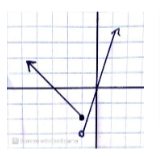
\includegraphics[width=\textwidth]{imgs/ex1.png}
\end{minipage}
\hspace{0.05\textwidth}
\begin{minipage}{0.6\textwidth}
    $\text{1. Given that}$
    $$f(x)=\left\{\begin{array}{c}
    -x-3, x \leq 1 \\
    3 x, x>-1
    \end{array}\right\},$$
    $\text{use a graphing approach to determine} \lim\limits_{x \to -1} f(x)$ or justify that it does not exist.
    $\lim_{x \to -1^-}f(x)=-2$\\
    $\lim_{x\ \to -1^+}f(x)=-3$\\
   $\boxed{\therefore\ \lim\limits_{x \to -1} f(x)\text{ does not exist}}$
    \vspace{1cm}
\end{minipage}
Evaluate the following using a graphing approach:
\[
\lim_{x \to 2}\left(\sqrt{x-2}+3\right)
\]
\noindent
\begin{minipage}[t]{0.5\textwidth}
    \vspace{0pt}
    \begin{tikzpicture}
        \begin{axis}[
            xlabel=$x$,
            ylabel={$f(x)$},
            axis lines=middle,
            xmax=4,
            ymax=6,
            xmin=0,
            ymin=0,
            xtick={0,1,...,4},
            ytick={0,1,...,6},
            grid=both,
            domain=2:4,
            samples=100,
            smooth,
            legend pos=north west,
        ]
            \addplot[blue,thick] {sqrt(x-2) + 3};
        \end{axis}
    \end{tikzpicture}
\end{minipage}
\hfill
\begin{minipage}[t]{0.4\textwidth}
    \vspace{0pt}
    \begin{align*}
        \lim_{x \to 2^-}\left(\sqrt{x-2}+3\right) &= 3 \\
        \therefore \lim_{x \to 2}\left(\sqrt{x-2}+3\right) &= 3
    \end{align*}
\end{minipage}
\newpage 
\subsection{Limits as x goes to Negative infinity or Infinity}
We previously discussed how to evaluate limits as x goes to infinity or as x goes to negative infinity using a graphing approach.\\
However, we can discuss how to evaluate these types of limits without using a graphing approach every time.\\
To discuss how to do this, we will look at some graphs.
It is NOT important to know the numbers of the scenarios that follow.

\subsubsection{Scenario 1}
\begin{minipage}[t]{0.5\textwidth}
    \vspace{0pt}
    Suppose $y=a^x, 0 <a<1$\\
    For example, suppose $y=\left(\frac{1}{2}\right)^x$\\
    $\lim_{x \to -\infty}f(x)=\infty$\\
    $\lim_{x \to \infty}f(x)=0$
\end{minipage}
\begin{minipage}[t]{0.45\textwidth}
    \vspace{0pt}
    \begin{tikzpicture}[scale=0.8]
        \draw[->] (-3,0) -- (3,0) node[below] {$x$};
        \draw[->] (0,-1) -- (0,3) node[left] {$f(x)$};
        \draw[domain=-2:3,smooth,variable=\x,blue] plot ({\x},{0.5^\x});
        \draw[dashed] (-3,2) -- (3,2) node[right] {$1$};
        \draw[dashed] (-2,0) -- (-2,0.5) node[above] {$a$};
    \end{tikzpicture}
\end{minipage}

\subsubsection{Scenario 2}
\begin{minipage}[t]{0.5\textwidth}
    \vspace{0pt}
    Suppose $y=a^x, a>1$\\
    For example, suppose $y=2^x$\\
    $\lim_{x \to -\infty}f(x)=0$\\
    $\lim_{x \to \infty}f(x)=\infty$
\end{minipage}
\begin{minipage}[t]{0.45\textwidth}
    \vspace{0pt}
    \begin{tikzpicture}[scale=0.8]
        \draw[->] (-3,0) -- (3,0) node[below] {$x$};
        \draw[->] (0,-1) -- (0,3) node[left] {$f(x)$};
        \draw[domain=-2:2,smooth,variable=\x,blue] plot ({\x},{2^\x});
        \draw[dashed] (-3,1) -- (3,1) node[right] {$1$};
        \draw[dashed] (-2,0) -- (-2,2) node[above] {$a$};
    \end{tikzpicture}
\end{minipage}

\subsubsection{Scenario 3}
\begin{minipage}[t]{0.5\textwidth}
    \vspace{0pt}
    Suppose $y=a^x, a=1$\\
    $\lim_{x \to -\infty}f(x)=1$\\
    $\lim_{x \to \infty}f(x)=1$
\end{minipage}
\begin{minipage}[t]{0.45\textwidth}
    \vspace{0pt}
    \begin{tikzpicture}[scale=0.8]
        \draw[->] (-3,0) -- (3,0) node[below] {$x$};
        \draw[->] (0,-1) -- (0,3) node[left] {$f(x)$};
        \draw[domain=-3:3,smooth,variable=\x,blue] plot ({\x},{1^\x});
        \draw[dashed] (-3,1) -- (3,1) node[right] {$1$};
        \draw[dashed] (-2,0) -- (-2,1) node[above] {$a$};
    \end{tikzpicture}
\end{minipage}

\subsubsection{Scenario 4}
\begin{minipage}[t]{0.5\textwidth}
    \vspace{0pt}
    Suppose $y=x^a, a>0$\\
    $\lim_{x \to \infty}f(x)=\infty$
\end{minipage}
\begin{minipage}[t]{0.45\textwidth}
    \vspace{0pt}
    \begin{tikzpicture}[scale=0.8]
        \draw[->] (0,0) -- (3,0) node[below] {$x$};
        \draw[->] (0,0) -- (0,3) node[left] {$f(x)$};
        \draw[domain=0.1:3,smooth,variable=\x,blue] plot ({\x},{\x});
        \draw[dashed] (0,0) -- (3,3) node[right] {$x^a$};
    \end{tikzpicture}
\end{minipage}

\subsubsection{Scenario 5}
\begin{minipage}[t]{0.5\textwidth}
    \vspace{0pt}
    Suppose $y=x^a, a<0$\\
    For example, suppose $y=x^{-1/2}$ or $y=-2$\\
    $\lim_{x \to \infty}x^a=0$
\end{minipage}
\begin{minipage}[t]{0.45\textwidth}
    \vspace{0pt}
    \begin{tikzpicture}[scale=0.8]
        \draw[->] (0,0) -- (3,0) node[below] {$x$};
        \draw[->] (0,0) -- (0,3) node[left] {$f(x)$};
        \draw[domain=0.3:3,smooth,variable=\x,blue] plot ({\x},{1/\x});
        \draw[dashed] (0,0) -- (3,0) node[right] {$x^a$};
    \end{tikzpicture}
\end{minipage}

\subsubsection{Scenario 6}
\begin{minipage}[t]{0.5\textwidth}
    \vspace{0pt}
    Suppose $y=a^x, a=0$\\
    $\lim_{x \to \infty}f(x)=1$
\end{minipage}
\begin{minipage}[t]{0.45\textwidth}
    \vspace{0pt}
    \begin{tikzpicture}[scale=0.8]
        \draw[->] (0,0) -- (3,0) node[below] {$x$};
        \draw[->] (0,0) -- (0,3) node[left] {$f(x)$};
        \draw[domain=0:3,smooth,variable=\x,blue] plot ({\x},{1});
        \draw[dashed] (0,1) -- (3,1) node[right] {$a^x$};
    \end{tikzpicture}
\end{minipage}

\newpage
\textbf{\underline{Limits of Rational Functions as \( x \) Approaches Infinity or Negative Infinity:}}

When evaluating the limit of a rational function as \( x \) approaches either infinity or negative infinity (i.e., a polynomial over another polynomial), the following approach can be employed:

\begin{enumerate}
    \item Determine the degrees of the numerator and denominator. Factor out \( x^n \) from both the numerator and denominator, where \( n \) is the greater or lesser of the two degrees. If both degrees are the same, \( n \) equals that degree. (Factor out the same term from both the numerator and denominator.) Cancel out like factors.
    
    \item Determine the limit of each term in the numerator and sum those limits. Determine the limit of each term in the denominator and sum those limits.
    \begin{enumerate}
        \item A numerator with a finite limit over a denominator growing without bound yields a limit of 0.
        
        \item A numerator with a finite limit over a denominator with a finite limit produces a limit equal to the quotient of those limits.
        
        \item A numerator with a finite limit over a denominator that tends to zero yields a limit of infinity or negative infinity.
        
        \item A numerator growing without bound over a denominator that's finite or tends to zero produces a limit of infinity or negative infinity.
        
        \item A numerator that tends to zero over a denominator that's finite or growing without bound yields a limit of 0.
    \end{enumerate}
\end{enumerate}
\subsection{Continuity}

The idea of continuity can be thought of informally as the idea of being able to draw a graph without lifting one’s pencil.\\
Three types of discontinuity are illustrated below.

\begin{figure}[h]
\centering
\begin{minipage}{0.3\textwidth}
\centering
\begin{tikzpicture}[scale=0.8]
  % Axes
  \draw[->] (-1.5,0) -- (1.5,0) node[right] {$x$};
  \draw[->] (0,-1.5) -- (0,1.5) node[above] {$y$};
  
  % Hole
  \draw[fill=white] (0.75,0.75) circle [radius=0.03];
  \draw[dashed] (0.75,0.75) circle [radius=0.03];
  
  % Labels
  \node[below right] at (0.75,0.75) {$\circ$ Hole};
\end{tikzpicture}
\caption*{Graph with a Hole}
\end{minipage}%
\hfill
\begin{minipage}{0.3\textwidth}
\centering
\begin{tikzpicture}[scale=0.8]
  % Axes
  \draw[->] (-1.5,0) -- (1.5,0) node[right] {$x$};
  \draw[->] (0,-1.5) -- (0,1.5) node[above] {$y$};
  
  % Jump Discontinuity
  \draw[fill=white] (-0.75,-0.75) circle [radius=0.03];
  \draw[fill=black] (-0.75,0.75) circle [radius=0.03];
  \draw[dashed] (-0.75,-0.75) -- (-0.75,0.75);
  
  % Labels
  \node[below left] at (-0.75,-0.75) {$\bullet$};
  \node[above left] at (-0.75,0.75) {$\bullet$};
  \node[above right] at (-0.75,0.75) {Jump Discontinuity};
\end{tikzpicture}
\caption*{Graph with a Jump Discontinuity}
\end{minipage}%
\hfill
\begin{minipage}{0.3\textwidth}
\centering
\begin{tikzpicture}[scale=0.8]
  % Axes
  \draw[->] (-1.5,0) -- (1.5,0) node[right] {$x$};
  \draw[->] (0,-1.5) -- (0,1.5) node[above] {$y$};
  
  % Vertical Asymptote
  \draw[dashed] (1,-1.5) -- (1,1.5);
  
  % Labels
  \node[above right] at (1,1.5) {Vertical Asymptote};
\end{tikzpicture}
\caption*{Graph with a Vertical Asymptote}
\end{minipage}
\end{figure}
\[
\boxed{\text{The function } f \text{ is continuous at } x=a \text{ if } f(a) \text{ is defined and if } f(a) = \lim_{x\to a} f(x)}
\]

\subsubsection{General Observations Regarding Continuity:}
\begin{enumerate}
    \item A function that is not continuous has some type of break in its graph.  This break is the result of a hole, jump, or vertical asymptote.
\item All polynomial functions are continuous for all real numbers.
\item A rational function $h(x)=\frac{f(x)}{g(x)}$is continuous at $x=a$ if $g(a)\neq 0$
\item A rational function in simplified for has a discontinuity at the zeros of the denominator.
\item When the one-sided limits are not equal to each other, then the limit at this point does not exist and the function is not continuous at this point
\end{enumerate}
\subsection{Properties of Limits}
\begin{itemize}
\item 1) $\lim _{x \rightarrow a} x=a$ \\
\item 2) $\lim _{x \rightarrow a} c=c$ \\
\item 3) $\lim _{x \rightarrow a}[c f(x)]=c \lim _{x \rightarrow a} f(x)$ \\
\item 4) $\lim _{x \rightarrow a}[f(x) \pm g(x)]=\lim _{x \rightarrow a} f(x) \pm \lim _{x \rightarrow a} g(x)$\\
\item 5) $\lim _{x \rightarrow a}[f(x) g(x)]=\lim _{x \rightarrow a} f(x) \lim _{x \rightarrow a} g(x)$\\
\item 6) $\lim _{x \rightarrow a} \frac{f(x)}{g(x)}=\frac{\lim _{x \rightarrow a} f(x)}{\lim _{x \rightarrow a} g(x)}$, only if $\lim _{x \rightarrow a} g(x) \neq 0$\\
\item 7) $\lim _{x \rightarrow a}[f(x)]^n=\left[\lim _{x \rightarrow a} f(x)\right]^n$\\

\item Where $\mathrm{c}$ is a constant, $\lim _{x \rightarrow a} f(x)$ and $\lim _{x \rightarrow a} g(x)$ exist.\\

\item If $P(x)$ is a polynomial, then
$$\lim _{x \rightarrow a} P(x)=P(a)$$
\end{itemize}

\newpage

\section{Unit 2 - Derivatives}
\subsection{Instantaneous Rate of Change, aka Tangent Lines, Slope at a Point, Derivatives}
\underline{Tangent Lines:} A tangent line to a curve is the straight line that most resembles the graph near that point.  By finding the slope of a tangent line, we can find the slope of the curve at the given point. \\ \\ 
Here are some examples of tangent lines:

\begin{tikzpicture}[scale=0.6]
  \draw[latex-latex, very thick] (-5.5,0)--(15.5,0);

  \draw[domain=-5:15,samples=200,smooth,variable=\x, blue, very thick] plot ({\x},{1+2*sin(\x r)});
 
  \draw[domain=-5:-3,smooth,variable=\x, orange, thick] plot ({\x},{2*\x*cos(4 r) + 1 - 2*sin(4 r) + 8*cos(4 r)});
  \node[above right] at (-4,{1+2*sin(-4 r)}) {decreasing quickly};
 
  \draw[domain=-2.5:-.5,smooth,variable=\x, orange, thick] plot ({\x},{1+2*sin(-1.57 r)});
  \node[below right] at (-1.57,{1+2*sin(-1.57 r)}) {no change};
 
  \draw[domain=0.5:3.5,smooth,variable=\x, orange, thick] plot ({\x},{3.76562-0.4544*\x});
  \node[above right] at (1.8,{1+2*sin(1.8 r)}) {decreasing slowly};
 
  \draw[domain=5.4:7.4,smooth,variable=\x, orange, thick] plot ({\x},{1.98637*\x - 11.4797});
  \node[below right,text width=2cm] at (6.4,{1+2*sin(6.4 r)}) {increasing quickly};
 
  \draw[domain=6.5:9,smooth,variable=\x, orange, thick] plot ({\x},{1+2*sin(7.85 r)});
  \node[above right] at (7.85,{1+2*sin(7.85 r)}) {no change};
 
  \draw[domain=10:12.5,smooth,variable=\x, orange, thick] plot ({\x},{0.40601*\x - 5.50566});
  \node[below right,text width=2cm] at (11.2,{1+2*sin(11.2 r)}) {increasing slowly};
\end{tikzpicture}
Up until now, we have talked about needing two points to determine the slope of a line. However, as we begin talking about derivatives, we need to talk about the slope of a curve at a certain point. \\
Suppose that we wish to determine the slope of the curve $y=f(x)$ at the point where $x=a$. This is the same as finding the slope of the line tangent to the curve $y=f(x)$ at $x=a$.\\
When $x=a$, $y=f(x)$.  Therefore, we will be trying to determine the slope of the curve $y=f(x)$ at the point $(a, f(a))$.

\begin{center}
    
\begin{tikzpicture}[>=Stealth]
  \draw[->] (-1,0) -- (5,0) node[right] {$x$};
  \draw[->] (0,-1) -- (0,5) node[above] {$y$};
  
  \draw[scale=1,domain=-1:3.5,smooth,variable=\x,blue] plot ({\x},{0.5*\x*\x});
  
  \fill[red] (1,{0.5*1*1}) circle (2pt) node[above left] {$(x, f(x))$};
  \fill[red] (3,{0.5*3*3}) circle (2pt) node[above left] {$(x+h, f(x+h))$};
  
  \draw[red, thick, shorten <=-1cm,shorten >=-1cm] (1,{0.5*1*1}) -- (3,{0.5*3*3});
  
  \draw[|<->|] (1,-0.5) -- node[below] {$h$} (3,-0.5);
  
  \draw[|<->|,purple] (3,{0.5*3*3}) -- node[right] {$f(x+h)-f(x)$} (3,{0.5*1*1});
  
  \draw[dashed] (1,{0.5*1*1}) -- (1,0) node[below] {$x$};
  \draw[dashed] (3,{0.5*3*3}) -- (3,0) node[below] {$x+h$};
  \draw[dashed] (3,{0.5*3*3}) -- (0,{0.5*3*3}) node[left] {$f(x+h)$};
  \draw[dashed] (1,{0.5*1*1}) -- (0,{0.5*1*1}) node[left] {$f(x)$};

  \node at (5,4) [align=left] {Slope of the \\ tangent line:\\ $\frac{f(x+h)-f(x)}{h}$};
  
\end{tikzpicture}
\end{center}
    
\begin{tcolorbox}[colback=Orchid!5!white,colframe=Orchid!75!white,coltitle=white,title=Slope of Tangent ]
The derivative of the function $y=f(x)$ is given formula
  \[
  f'(x)=\lim_{h \to 0} \frac{f(x+h)-f(x)}{h},
  \]
 Other symbols for the derivative include $y'$ and $\frac{\delta y}{\delta x}$
\end{tcolorbox}
The derivative of a function allows you to determine the slope of the line tangent to a curve at a given point. In other words, you can find the slope of the line when you only know one point on the line. The value of the derivative is often called the instantaneous rate of change.
\subsubsection*{Example:}
Determine the derivative of the function $y=x^2$ and evaluate the derivative at the point where $x=3$.\\ \\ 
\textbf{Solution:}
\begin{align*}
    y' &= \lim_{x \to 0} \frac{f(x+h)-f(x)}{h}\\
    &= \lim_{h \to 0} \frac{(x+h)^2-x^2}{h}\\
    &= \lim_{h \to 0} \frac{x^2+2xh+h^2-x^2}{h}\\
    &= \lim_{h \to 0} \frac{2xh+h^2}{h}\\
    &= \lim_{h \to 0} (2x+h)\\
    &= 2x + 0\\
    &= 2x.\\
    & \therefore y'=2x, \text{ at } x=3. \\
    y' &=2(3)=6 
\end{align*}
By evaluating the limit as the change in \( x \) approaches zero, we find the derivative \( y' = 2x \). Therefore, at \( x = 3 \), the derivative equals 6.
\newpage
\subsubsection*{Example:}
Determine the equation of the tangent line to the curve $y=x^2$ at the point where $x=3$. \\ \\ 
\textbf{Solution:}
\begin{align*}
    y &= mx + b, \quad \text{we know } m = 6 \\
    y &= 6x + b \\
    & \text{Substitute }(3, 9): \\
    9 &= 6(3) + b \\
    -9 &= b \\
\end{align*}
Therefore, the equation of the tangent at \(x = 3\) is \(y = 6x - 9\).
\subsubsection*{Example:}
Give that $y=3x^2-7x+6$, determine the value of $\frac{\delta y}{\delta x}$ at $x=5$. \\ \\ 
\textbf{Solution:}
\begin{align*}
    f'(x)&=\lim_{h to 0} \frac{f(x+h)-f(x)}{h}\\
    &=\lim_{h to 0} \frac{3(x+h)^2-7(x+h)+6-(3x^2-7x+6)}{h}\\
    &=\lim_{h to 0} \frac{3(x^2+2xh+h^2)-7x+7h+6-3x^2+7x-6}{h}\\
    &=\lim_{h to 0} \frac{\cancel{3x^2}+6xh+3h^2\cancel{-7x}+7h\cancel{+6}\cancel{-3x^2}\cancel{+7x}\cancel{-6}}{h}\\
    &= \lim_{h to 0} \frac{6hx+3h^2-7h}{h}\\
    &= \lim_{h to 0} \frac{\cancel{h}(6x+3h-7)}{\cancel{h}}\\
    &=6x+3(0)-7\\
    &= 6x-7
\end{align*}
At $x=5$ 
\begin{align*}
    &\frac{\delta y}{\delta x}=6(5)-7\\
    &=23
\end{align*}
\newpage
\subsubsection*{Example:}
Determine the equation of the tangent line of the curve $f(x)= \frac{1}{x}$ at the point where $x=2$.\\ \\ 
\textbf{Solution:}
\begin{align*}
    f'(x) &=\lim_{h \to 0}\frac{f(x+h)-f(x)}{h}\\
    &=\lim_{h \to 0}\frac{\frac{1}{x+h}-\frac{1}{x}}{h}\\
    &=\lim_{h \to 0} \frac{\frac{x}{x(x+h)} -\frac{(x+h)}{x(x+h)}}{h}\\
    &=\lim_{h \to 0} \frac{x-(x+h)}{xh(x+h)}\\
    &=\lim_{h \to 0} \frac{x-x-h}{xh(x+h)}\\
    &=\lim_{h \to 0} \frac{\cancel{h}}{x\cancel{h}(x+h)}\\
    &=\frac{-1}{x(x+0)}\\
    &=\frac{-1}{x^2}
\end{align*}
At $x=3$, $y=\frac{1}{2}$. Therefore, the point is $\left(2,\frac{1}{2}\right)$.\\
The derivative is $\frac{-1}{x^2}$. Therefore, the slope at $x=2$ is $\frac{-1}{2^2}=\frac{-1}{4}$
\begin{align*}
    &= y=mx+b\\
    &= y=\frac{-1}{4}x+b\\
    & \text{Sub in} \left(2,\frac{1}{2}\right)\\
    \frac{1}{2} &= \frac{-1}{4}(2)+b\\
    1 &=b
\end{align*}
The equation of the tangent line is $y=-\frac{1}{4}x+1$
\newpage 
\subsubsection*{Example:}
Determine an equation of the line that is perpendicular to the tangent to the graph of $f(x)=\frac{1}{x}$ at the point where $x=2$ and that intersects it at the point of tangency.(this is called the normal) \\  \\ 
\textbf{Solution:}

Our point is still $\left(2,\frac{1}{2}\right)$, our perpendicular slope is the negative reciprocal of the $-1\frac{1}{4}$, which is 4.
\begin{align*}
    &\therefore y=4x+b\\
    &\text{sub in} \left(2,\frac{1}{2}\right)\\
    \frac{1}{2}&=4(2)+b\\
    \frac{-15}{2}&=b\\
\end{align*}
The equation of the normal is $y=4x-\frac{15}{2}$
\subsection*{The Existence of Derivatives:}
A function $f$ is said to be differentiable at $x=a$ if $f'(a)$ exists. At points where $f$ is not differentiable, we say that the derivative does not exist. Common ways for a derivative to not exist are shown.

\begin{figure}[h]
\centering
\begin{minipage}[b]{0.5\textwidth}
\centering
\begin{tikzpicture}[scale=0.5]
  % Cusp
  \draw[->] (-2,0) -- (2,0) node[right] {$x$};
  \draw[->] (0,-2) -- (0,2) node[above] {$y$};
  \draw[domain=-1.5:1.5, smooth, variable=\x, blue] plot ({\x}, {\x*\x});
  \node[below right, blue] at (0,0) {Cusp};
\end{tikzpicture}
\end{minipage}%
\begin{minipage}[b]{0.5\textwidth}
\centering
\begin{tikzpicture}[scale=0.5]
  % Vertical tangent
  \draw[->] (-2,0) -- (3,0) node[right] {$x$};
  \draw[->] (0,-2) -- (0,2) node[above] {$y$};
  \draw[domain=-1.5:2.5, smooth, variable=\x, blue] plot ({\x}, {\x/(1+\x*\x)});
  \node[below right, blue] at (0,0) {Vertical Tangent};
\end{tikzpicture}
\end{minipage}\\[20pt]
\begin{minipage}[b]{0.5\textwidth}
\centering
\begin{tikzpicture}[scale=0.5]
  % Hole
  \draw[->] (-2,0) -- (2,0) node[right] {$x$};
  \draw[->] (0,-1.5) -- (0,1.5) node[above] {$y$};
  \draw[domain=-1.5:1.5, smooth, variable=\x, blue] plot ({\x}, {(\x-1)*(\x+1)});
  \node[above right, blue] at (0,0) {Hole};
\end{tikzpicture}
\end{minipage}%
\begin{minipage}[b]{0.5\textwidth}
\centering
\begin{tikzpicture}[scale=0.5]
  % Corner
  \draw[->] (-2,0) -- (2,0) node[right] {$x$};
  \draw[->] (0,-1.5) -- (0,1.5) node[above] {$y$};
  \draw[domain=-1.5:1.5, variable=\x, blue] plot ({\x}, {abs(\x)});
  \node[below left, blue] at (0,0) {Corner};
\end{tikzpicture}
\end{minipage} 
\caption{Different Types of Discontinuities}
\label{fig:discontinuities}
\end{figure}


\section*{No Derivative}
\begin{minipage}[h]{0.7\textwidth}
  \centering
  \begin{tikzpicture}[scale=0.7]
    \draw[latex-latex, very thick] (-5.3,0)--(5.3,0);
    \draw[latex-latex, very thick] (0,-5.3)--(0,5.3);
  
    \draw[domain=2.0001:5,samples=300,smooth,variable=\x, blue,  thick] plot ({\x},{2*exp(ln(\x-2)/3)});
    \draw[domain=2.0001:5,samples=300,smooth,variable=\x, blue,  thick,rotate around={180:(2,0)}] plot ({\x},{2*exp(ln(\x-2)/3)});
    \draw[blue,thick] (2,-0.1)--(2,0.1);
    \draw[domain=-5:-1,samples=300,smooth,variable=\x, blue,  thick] plot ({\x},-1.2*\x*\x-8*\x-9.68);
    \draw[orange,thick](-1,-2.88) circle (0.45);
    \draw[orange,thick](2,0) circle (0.45);
    \node[left] at (-1.3,-3.4) {Cusp};
    \node[above right] at (2.2,0.3) {Vertical Tangent Line};
  \end{tikzpicture}
\end{minipage}%
\begin{minipage}[t]{0.5\textwidth}
This graph represents a function that is not differentiable at certain points. The presence of a cusp and vertical tangent lines indicates that the function lacks a derivative at those points.
\end{minipage}

\section*{Inverse Derivative}
\begin{minipage}[h]{0.7\textwidth}
  \centering
  \begin{tikzpicture}[scale=0.7]
    \draw[black!30!white, very thin] (-5,-5) grid (5,5);
    \draw[latex-latex, very thick] (-5.3,0)--(5.3,0);
    \draw[latex-latex, very thick] (0,-5.3)--(0,5.3);
    
    \begin{scope}
        \clip (-5,-5) rectangle (5,5);
        \draw[very thick, OliveGreen,dotted](-5,-5)--(5,5);
        \node[OliveGreen,below right] at (4,4) {$y=x$};
        
        \draw[domain=-5:1.4,smooth,variable=\x, RoyalPurple, ultra thick] plot ({\x},{exp(\x)+1});
        \node[RoyalPurple,above] at (-3,1) {$f(x)$};
        \draw[RoyalPurple,fill=RoyalPurple] (0.5,2.649) circle [radius=0.2];
        \draw[domain=-4.5:2,smooth,variable=\x, DarkOrchid, ultra thick,dashed] plot ({\x},{1.649*\x+1.824});
        
        \draw[domain=1.003:5,smooth,variable=\x, NavyBlue, ultra thick, samples=150] plot ({\x},{ln(\x-1)});
        \node[NavyBlue,right] at (1,-3) {$f^{-1}(x)$};
        \draw[NavyBlue,fill=CornflowerBlue] (2.649,0.5) circle [radius=0.2];
        \draw[domain=-5:5,smooth,variable=\x, Cerulean, ultra thick,dashed] plot ({\x},{0.606*\x-1.105});
    \end{scope}
  \end{tikzpicture}
\end{minipage}%
  \vspace{2em}
\begin{minipage}[h]{0.5\textwidth}
This graph represents the inverse function of a function that has a derivative. The presence of a straight line indicates that the inverse function is linear. Additionally, the graph illustrates that the inverse function reverses the behavior of the original function with respect to the line $y=x$.
\end{minipage}



\subsection{Power Rule}
\begin{tcolorbox}[sharp corners=uphill,
    colback=purple!50!white,colframe=blue!25!black,coltext=yellow,
    fontupper=\Large\bfseries,arc=6mm,boxrule=2mm,boxsep=5mm]
  if $f(x)=x^{n}$, then $f'(x)=nx^{n-1}$
\end{tcolorbox}
  \textit{Proof}\\
  \begin{align*}
    f'(x)&=\lim_{h \to 0}\frac{f(x+h)-f(x)}{h}\\
    & \text{if } f(x)=x^n\\
    & \text{Then, } f(x+h)= (x+h)^n 
  \end{align*}
\subsubsection*{Example:}
if $f(x)= 4x^5$, then determine $f'(x)$. \\ \\ 
\textbf{Solution:}
\begin{align*}
    &= 4x^5\\
    &= (5)(4)x^{5-1}\\
    &=20x^4
\end{align*}
\subsubsection*{Example:}
if $f(x)= 11x^{\frac{5}{2}}$, then determine $f'(x)$.\\ \\ 
\textbf{Solution:}
\begin{align*}
    &= 11x^{\frac{5}{2}}\\
    &= \left(\frac{5}{2}\right)(10)x^{\frac{5}{2}-1}\\
    &= \frac{55}{2}x^{\frac{3}{2}}\\
\end{align*}
\subsubsection*{Example:}
if $f(x)=7x$, then determine $f'(x)$.\\ \\ 
\textbf{Solution:}
\begin{align*}
    &=(0)(7)x^{0-1}\\
    &=0
\end{align*}
\newpage
\subsection{Product Rule}
\begin{tcolorbox}[colback=Orchid!5!snow, colframe=nadeshikopink!50!white,
  colbacktitle=mordantred19!75!mistyrose, title=Product Rule]

The product rule states that if $p(x)=f(x)g(x)$, then\\ $p'(x)=f'(x)g(x)+f(x)g'(x)$.
\textbf{Product Rule in Newton Notation.}\\


$\frac{\delta}{\delta x}(uv)=\left(\frac{\delta u}{\delta x}\right)v+u\left(\frac{\delta v}{\delta x}\right)$
\textbf{Product Rule in Leibniz Notation}

\end{tcolorbox}
\textit{Proof of the Product Rule}
\begin{align*}
    p'(x) &= \lim_{h \to 0}\frac{p(x+h)-p(x)}{h}\\
    &=\lim_{h \to 0}\frac{f(x+h)g(x+h)-f(x)g(x)}{h}\\
    &=\lim_{h \to 0}\frac{f(x+h)g(x+h)\textcolor{red}{-f(x)g(x+h)+f(x)g(x+h)}-f(x)g(x)}{h}\\
    &= \lim_{h \to 0}\left[\frac{f(x+h)-f(x)}{h}\right]g(x+h)+f(x)\left[\frac{g(x+h)-g(x)}{h} \right]\\
    &=\left(\lim_{h \to 0} \frac{f(x+h)-f(x)}{h} \right) \left[\lim_{h \to 0}g(x+h)\right]+\left[\lim_{h \to 0} f(x)\right]\left(\lim_{h \to 0}\frac{g(x+h)-g(x)}{h}  \right)\\
    &=f'(x)g(x)+f(x)g'(x)
\end{align*}
\subsection*{Example}
Differentiate $h(x)=(x^3-2x)(3x^4+2x+8)$.\\
\textbf{Solution:}
$h'(x)=(3x^2-2)(3x^4+2x+8)+(x^3-2x)(12x^3+2)$.

Because of the power rule, we are able to say that the derivative of $kf(x)$ where is a scalar is $kf'(x)$.  In other words, we are able to just leave the scalar alone in front and determine the derivative of the function.\\
An example of this would be that if $y=7(3x^2+2x+6)$, then $$\frac{\delta y}{\delta x}=7(6x+2)$$\\
In other words, the derivative would equal 7 times the derivative of the polynomial.\\
How do we know this? By the power rule. Here’s the explanation.
Let $f(x)g(x)$, where $f(x)=7$ and $g(x)=3x^2+2x+6$.  

\begin{align}
    \frac{\delta y}{\delta x}&=f'(x)g(x)+f(x)g'(x)\\
    \frac{\delta y}{\delta x}&=(0)(3x^2+2x+6)+7(6x+2)\\
    &=7(6x+2)
\end{align}

\subsection{Quotient Rule}
"Low di high minus high di low over low low." \\
What does this mean? Well it means the quotient rule

\begin{tcolorbox}[colback=blue!5!snow, colframe=white!50!white,
  colbacktitle=blue!75!mistyrose, title=Quotient Rule]
if $h(x)=\frac{f(x)}{g(x)}$, then $h'(x)=\frac{f'(x)g(x)-f(x)g'(x)}{[g(x)]^2}, g \neq 0$\\
In Leibniz notation, $\frac{\delta }{\delta x}(\frac{u}{v})=\frac{\frac{\delta u}{\delta x}v- u\frac{\delta v}{\delta x}}{v^2}$
\end{tcolorbox}
\textit{Proof:}
\begin{align*}
    h(x)&=\frac{f(x)}{g(x)} \implies h(x)g(x)=f(x)\\
    & \therefore \text{by the product rule, } h'(x)g(x)+h(x)g'(x)=f(x)'\\
    &\implies h'(x)\cancel{g(x)}=\frac{f'(x)-h(x)g'(x)}{g(x)}\\
    &h'(x)=\frac{f'(x)-\left[\frac{f(x)}{g(x)}\right]g'(x)}{g(x)}\\
    &=\frac{f'(x)\left( \textcolor{red}{\frac{g(x)}{g(x)}}\right)-\frac{f(x)g'(x)}{g(x)}}{g(x)}\\
    &=\frac{\frac{f'(x)g(x)}{g(x)}-\frac{f(x)g'(x)}{g(x)}}{g(x)}\\
    &=\frac{f'(x)g(x)-f(x)g'(x)}{[g(x)]^2}
\end{align*}
\subsubsection*{Example:}
Determine the derivative of $h(x)=\frac{3x-4}{x^2+5}$.\\
\textbf{Solution:}
$h'(x)=\frac{(x^2+5)(3)-(3x+4)(4)}{(x^2+5)^ 2}$
\newpage 


\subsection{Chain Rule}
\begin{tcolorbox}[colback=OliveGreen!5!snow, colframe=white!50!white,
  colbacktitle=OliveGreen!75!mistyrose, title=Chain Rule]
The chain rule states 
if $h(x)=f \circ g(x)$, then $f'(g(x))g'(x)$ \\
$\frac{\delta y}{\delta x}=\frac{\delta y}{\delta u} \times \frac{\delta u}{\delta x}$
\end{tcolorbox}
\textit{Proof:}\\
\begin{align*}
\left[f(g(x)) \right]'&=\lim_{h \to 0} \frac{f(g(x+h)-f(g(x)))}{h}\\
&= \lim_{h \to 0} \left[ \frac{f(g(x+h)-f(g(x))}{\textcolor{red}{g(x+h)-g(x)}} \frac{\textcolor{red}{g(x+h)-g(x)}}{h}\right]\\
&=\lim_{h \to 0}\frac{f(g(x+h))-f(g(x))}{g(x+h)-g(x)} \lim_{h \to 0}\frac{g(x+h)-g(x)}{h}\\
&\boxed{\text{let k } = g(x+h)-g(x) \therefore \text{ as } h \to 0, k \to0}\\
&= \left[\lim_{\textcolor{red}{k \to 0}}\frac{f(g(x+\textcolor{red}{k})-f(g(x))}{\textcolor{red}{k}} \right]\left[ \lim_{h \to 0}\frac{g(x+h)-g(x)}{h}\right]\\
&=f'(g(x))g'(x)
\end{align*}
\subsubsection*{Example 1:}
Determine the derivative of $h(x)=(10x^3-7x^2+3x-9)^{14}$\\
\textbf{Solution:}
$h'(x)=14(10x^3-7x^2+3x-9)^{13}(30x^2-14x+3)$
\subsubsection*{Example 2:}
Suppose $f(12)=-7, g(3)=12, f'(12)=11$ and $g'(3)=9$. If $h(x)=f(g(x))$, then evaluate $h'(3)$.\\
\textbf{Solution:}
\begin{align*}
    h'(x)&=f(g(x))\\
    h'(3)&=f'(g(3))g'(3)\\
    &=f'(12)(9)\\
    &=(11)(9)\\
    &=99
\end{align*}
\newpage 

\subsection{Derivatives Not in Terms of $x$:}
Every time that we state a rate of change, we state that rate of change with respect to something.\\
For instance, if we talk about speed, we are talking about distance with respect to time.\\
When we discuss slope on a Cartesian plane, we use the formula:
$$m=\frac{y_2-y_1}{x_2-x_1}$$
In other words, we talk about the change in y with respect x.\\
Similarly, when we determine a derivative(which is just an instantaneous rate of change, or slope at a point), we determine the derivative with respect to something. Usually, we derivative with respect to x. However, this isn't always case.\\

The definition of a derivative is 
$$f'(x)=\lim_{h \to 0}\frac{f(x+h)-f(x)}{h}$$
The derivative is the limit of the slope between two points on a relation as those two points get infinitely close together. Alternatively, then we could define the derivative $$f'(x)= \lim_{x \to a }\frac{f(x)-f(a)}{x-a}$$

\subsubsection*{Example 1:}
Suppose $y=3(2x^2+x+-1)^4$. Determine $\frac{\delta y}{\delta x}$.\\
\textbf{Solution:}
$\frac{\delta y}{\delta x}=12(2x^2+x-1)^3(4x+1)$
\subsubsection*{Example 2:}
Suppose $y=3(2x^3+x-1)^4$. Determine $\frac{\delta y}{\delta(2x^2+x-1)}$.\\
\textbf{Solution:}
\begin{align*}
    \text{ let w } &= (2x^2+x-1)^4\\
    y&=3w^4\\
    \frac{\delta y}{\delta x}&=12w^3\\
    \frac{\delta y}{\delta(2x^2+x-1)}&=12(2x^2+x-1)^3
\end{align*}

\begin{center}
\begin{figure}
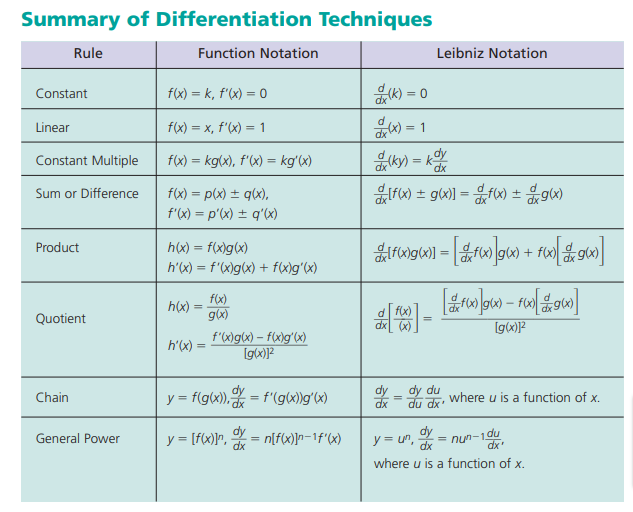
\includegraphics[width=1\textwidth]{imgs/summary of differentiation techniques.png}
\caption{Summary of Differentiation Techniques }
\end{figure}
\end{center}
\newpage 


\subsection{Implicit Differentiation}
Unit now, we have been determining derivatives when y is stated explicitly in terms of x.\\
However, sometimes are equation in terms of x, and remember to use the chain rule when differentiating terms containing y.\\
We may need to use other rules of differentiation as well.\\
\subsubsection{Intro to How Implicit Differentiation Works:}
\begin{itemize}
    \item The derivative pf $5x^3$ with respect to x is $15x^2$. We can think of this slightly differently though and say that the derivative of $5x^3$ with respect to x is $15x^2 \frac{\delta x}{\delta x}$ and that since $\frac{\delta x}{\delta x}=1$, therefore the derivative of $5x^3$ with respect to is $15x^2$
    \item By the same way of thinking, the derivative of $5y^3$ with respect to x is $15y^2 \frac{\delta y}{\delta x}$
\end{itemize}
\subsubsection*{Example}
If $x^2+y^2=25$, determine $\frac{\delta y}{\delta x}$ and determine the slope of the tangent to the curve at the point (3,-4).
\begin{align*}
    2x+2y \frac{\delta y}{\delta x}&=0\\
    2y \frac{\delta y}{\delta x}&=-2x\\
    \frac{\delta y}{\delta x}=\frac{-2x}{2y}\\
    \frac{\delta y}{\delta x}=\frac{-x}{y}\\
    \text{at }(3,-4), \frac{\delta y}{\delta x}&=\frac{-3}{-4}\\
    \frac{\delta y}{\delta x}=\frac{3}{4}
\end{align*}

\newpage 
\subsection{Related Rates}

\begin{itemize}
    \item After 1 second, the circular ripple would have an area of $\pi(1)^2=\pi m^2$ 
    \item After 2 seconds, the circular ripple would have an area of $\pi(2)^2=4\pi m^2$ (an increase of $3\pi m^2$)
    \item After 3 seconds, the circular ripple would have an area of $\pi(3)^2=9\pi m^2$ (an increase of $5\pi m^2$)
    \item After 4 seconds, the circular ripple would have an area of $\pi(4)^2=16\pi m^2$ (an increase of $7\pi m^2$)
\end{itemize}

We see that although the rate of increase of the radius remains constant, the rate of increase of the area is changing. The rate of increase of the area is related to the rate of increase of the radius. We call it a “related rate”. The rate of increase of the area is a function of time and it is not a constant.

Examples of Related Rates in Calculus
There are many types of related rates in Calculus. For example,
\begin{itemize}

\item Imagine a stone in a pond causing a circular ripple. The rate of increase of the area of the circular ripple will be related to the rate of increase of the radius of the ripple. If the rate of increase of the radius of the circular ripple is constant, the rate of increase of the area of the circular ripple will not be.

\item Imagine blowing air into a spherical balloon. The rate of increase of the radius of the sphere will be related to the rate of increase of the volume of the sphere. If the rate of increase of the volume of air in the sphere is constant, the rate of increase of the radius of the sphere will not be.

\item Imagine filling a cone shaped container with liquid. The rate of increase of the height of the liquid will be related to the rate of increase of the volume of the liquid in the cone. If the rate of increase of the volume of the liquid is constant, the rate of increase of the height of the liquid will not be.

There are many more examples.

\end{itemize}
\subsubsection{How To Approach a Related Rates Problem}
\begin{enumerate}
\item Some people like to draw a diagram.

\item Assign a variable to each quantity in the problem that is a function of the independent variable.  (We’ll assume for the remainder of this discussion that the independent variable is time)

\item Develop an equation that associates the variables with one another.4.Differentiate (possibly using implicit differentiation).

\item Substitute in given information and solve for the required rate of change.
\end{enumerate}
\subsubsection*{Example:} 
When a raindrop falls into a small puddle, it creates a circular ripple that spreads out from the point where the raundrop hit. The radius of the circle grows at a rate of 3 cm/s.
a) determine the rate of increase of the circumference of the circle with respect to time.\\
b) determine the rate of increase \\
\textbf{Solution:}

a) 
\begin{align*}
    \frac{\delta r}{dt}&=3\\
    C&=2\pi r\\
    \frac{\delta c }{\delta t}&=2 \pi \frac{\delta r}{\delta t}\\
    &=2 \pi (3cm/s)\\
    &=6 \pi cm/s 
\end{align*}
$\therefore$ the circumference increase at a rate of $6 \pi$ cm/s
b) 
\begin{align*}
    A&=\pi r^2\\
    \frac{\delta A}{\delta t} &=2\pi r \frac{\delta r}{\delta t}\\
    A&=81 \pi \\
    r^2&=81\\
    r&=9\\
    \frac{\delta A}{\delta t}&=2\pi (9 cm)(3cm/s)\\
    &=54\pi cm^2/s
\end{align*}

 
\subsubsection{How to approach each problem}
\begin{itemize}
    \item Identify the given variables and the quantities that need to be determined. Draw a picture if one is not given.

    \item Write an equation involving the rates whose variables are given or need to be determined. Do not substitute yet unless the value will never change.

    \item Using the chain rule, implicitly differentiate both sides of the equation with respect to time ($t$).

    \item Substitute into the resulting equation all known values for the variables and their rates of change. Then, solve for the required rate of change.	
\end{itemize}

\section{Unit 3 - Derivatives and Applications }
\subsection{Higher Order Derivatives, Velocity, Acceleration, and Rates of Change}
\subsubsection*{Second Derivative Test}
The second derivative of $y=f(x)$ is the derivative of $y=f^{\prime}(x)$\\
In Newton notation, the second derivative is $f^{\prime \prime}(x)$\\
In Leibniz notation, the second derivative is $\frac{d^2 y}{d x^2}$\\

\underline{Displacement:} The position of an object with respect to time, usually referred to as $s(t)$.\\

\underline{Velocity:} The rate of change of displacement over time. Therefore, the first derivative of the displacement function with respect to time is velocity.\\
$$
v(t)=s^{\prime}(t) \quad \text { or } \quad v(t)=\frac{d s}{d t}
$$

\underline{Acceleration:} The rate of change of velocity over time. Therefore, the first derivative of the velocity function with respect to time, or the second derivative of displacement with respect to time, is acceleration.\\
$$
a(t)=v^{\prime}(t)=s^{\prime \prime}(t) \quad \text { or } \quad a(t)=\frac{d v}{d t}=\frac{d^2 s}{d t^2}
$$

\underline{Some Points to Ponder About Velocity and Acceleration}
\begin{itemize}
\item Negative velocity means that an object is moving in a negative direction (left or down) while positive velocity means the opposite
\item Zero velocity means that an object is stationary and that a possible change in direction may occur.
\item Negative acceleration means that the velocity is decreasing, while positive acceleration means that the velocity is increasing.
\item Zero acceleration means that the velocity is constant
\item The speed of an object is the magnitude of its velocity.
$$
\text {Speed }=|v(t)|=\left|s^{\prime}(t)\right|
$$
\item An object is speeding up (increasing speed) when its velocity and acceleration have the same signs. However, an object is slowing down (decreasing speed) when its velocity and acceleration have opposite signs.
\item If the displacement is measured in metres and time is measured in seconds, then velocity is measured in $\mathrm{m} / \mathrm{s}$ and the acceleration is measured in $\mathrm{m} / \mathrm{s}^2$.
\end{itemize}



\subsubsection*{Concavity}

We know that the sign of the derivative tells us whether a function is increasing or decreasing at some point. Likewise, the sign of the second derivative $f''(x)$ tells us whether $f'(x)$ is increasing or decreasing at $x$. We summarize the consequences of this seemingly simple idea in the table below:


\begin{figure}[ht]
    \centering
    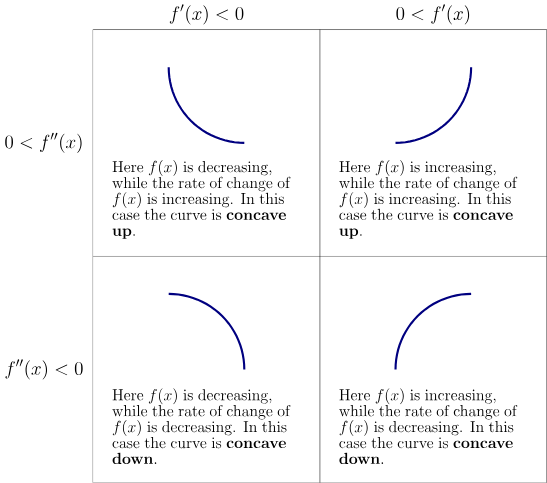
\includegraphics[width=0.7\textwidth]{imgs/digInConcavityAnd2ndDerivTest-figure0.png}
\end{figure}

The sign of the second derivative $f''(x)$ tells us about the behavior of the first derivative $f'(x)$:

\begin{center}
\begin{tabular}{@{}ll@{}}
\toprule
Sign of $f''(x)$ & Behavior of $f'(x)$ \\
\midrule
$f''(x) > 0$ & $f'(x)$ is increasing (concave up) \\
$f''(x) < 0$ & $f'(x)$ is decreasing (concave down) \\
\bottomrule
\end{tabular}
\end{center}



\newpage 

\subsubsection*{Example:}
\begin{center}
\begin{minipage}{\linewidth}
    \centering
    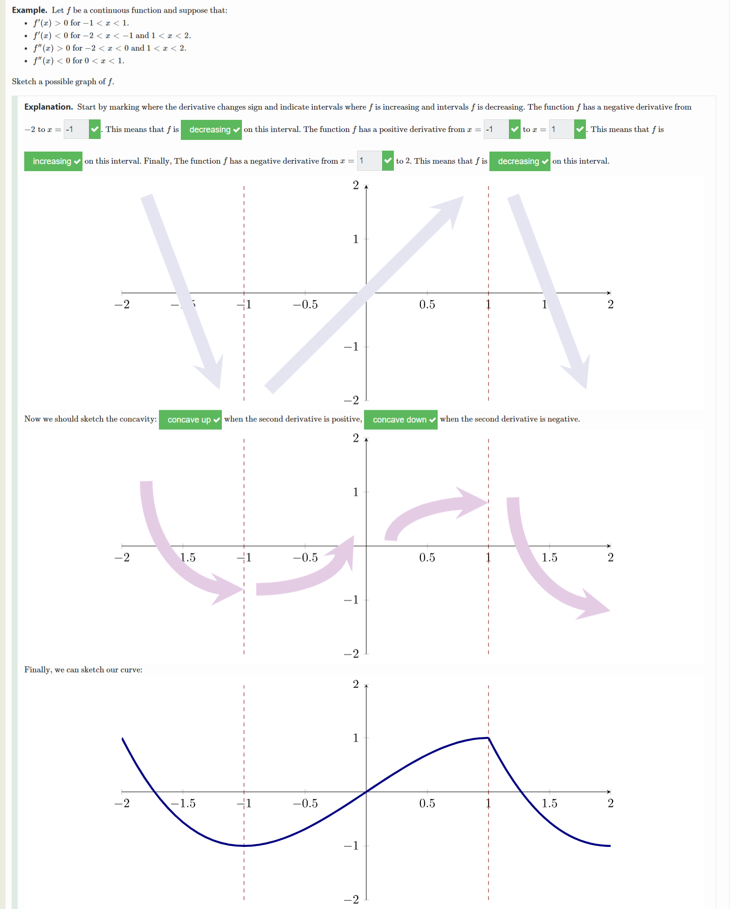
\includegraphics[width=1.3\textwidth]{imgs/ex.png}
\end{minipage}
\end{center}

\newpage 
\subsection{Inflection Points}
If we are trying to understand the shape of the graph of a function, knowing where it is concave up and concave down helps us to get a more accurate picture. Of particular interest are points at which the concavity changes from up to down or down to up.

\begin{tcolorbox}[sharp corners=uphill]
\underline{Definition:} If the concavity of $f$ changes either from up to down or down to up at $x=a$ and $f$ has a tangent line at $x=a$, then $x=a$ is an inflection point of $f$.
\end{tcolorbox}

It is instructive to see some examples of inflection points:

\begin{figure}[ht]
    \centering
    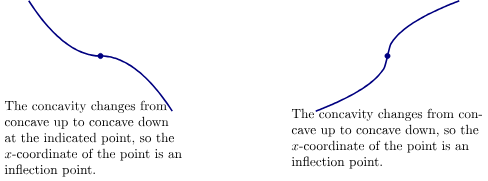
\includegraphics[width=0.7\textwidth]{imgs/digInConcavityAnd2ndDerivTest-figure4.png}
\end{figure}

\begin{figure}[ht]
    \centering
    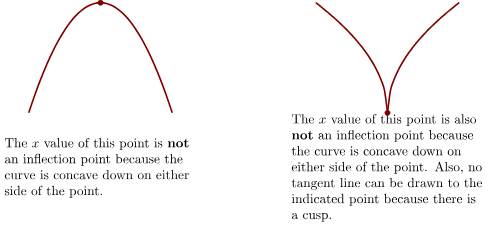
\includegraphics[width=0.7\textwidth]{imgs/digInConcavityAnd2ndDerivTest-figure5.png}
\end{figure}

\textcolor{red}{Warning:} Even if $f''(a)=0$, the point determined by $x=a$ might not be an inflection point. You also need to check that the concavity of $f$ changes on either side of $x=a$.
\newpage 

\subsubsection*{Example:}
\begin{center}
\begin{minipage}{\linewidth}
    \centering
    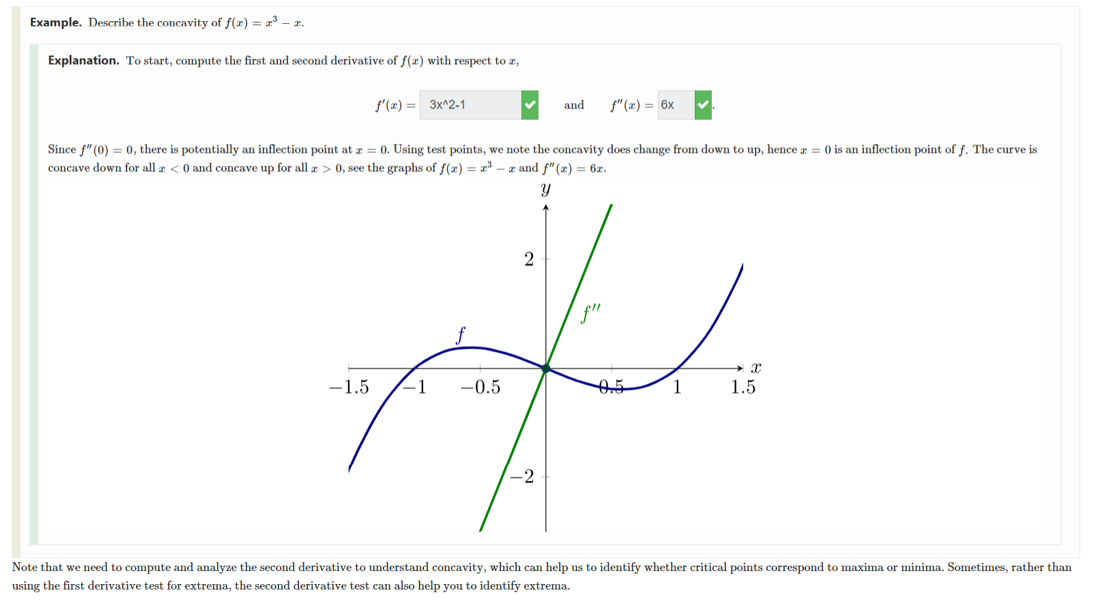
\includegraphics[width=1.3\textwidth]{imgs/ex3.png}
\end{minipage}
\end{center}
\underline{Problem:}
If $f''(a)=0$, what does the second derivative test tell us?


\begin{enumerate}
    \item[a)] The function has a local extrema at $x=a$
    \item[b)] The function does not have a local extrema at $x=a$
    \item[c)] It gives no information on whether $x=a$ is a local extremmum.
\end{enumerate}
The correct answer is C.
\subsubsection*{Example:}
\begin{center}
\begin{minipage}{\linewidth}
    \centering
    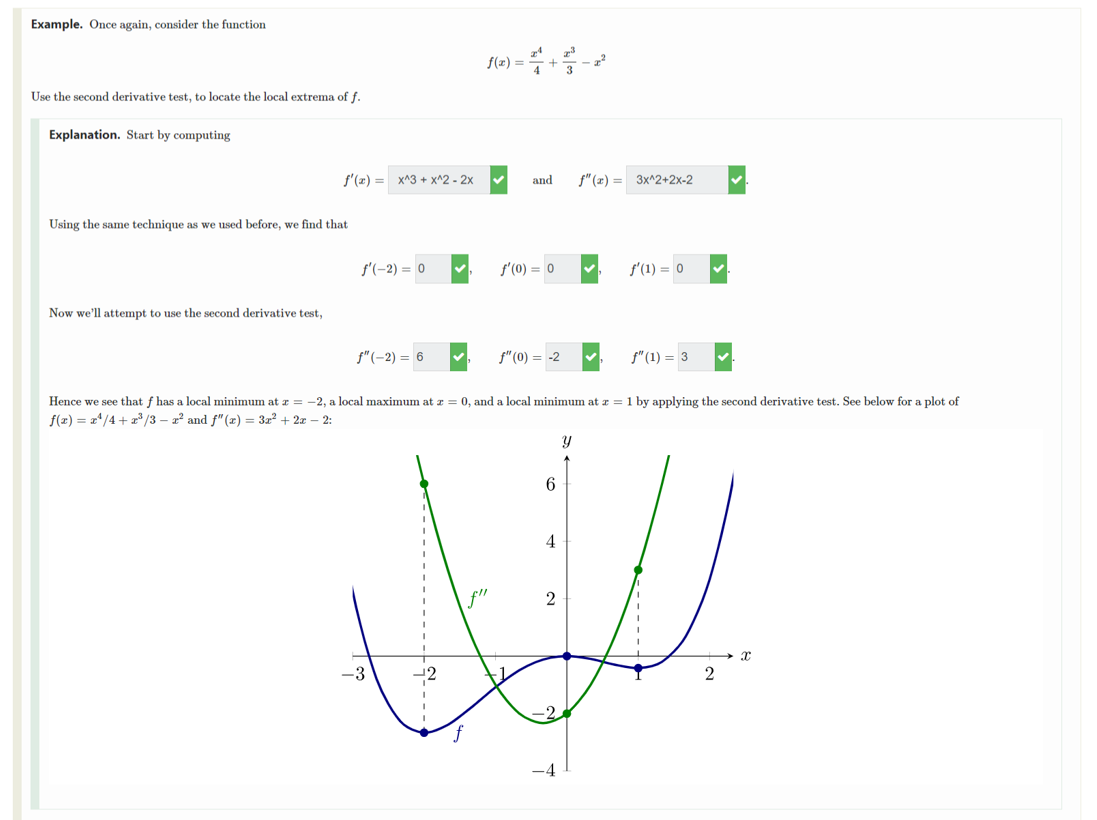
\includegraphics[width=1.3\textwidth]{imgs/ex4.png}
\end{minipage}
\end{center}
\underline{Second Derivative Test:}

\begin{itemize}
\item If $f'(c)=0$ and $f''(c)>0$, then there is a local minimum at $x=c$.
\item If $f'(c)=0$ and $f''(c)<0$, then there is a local maximum at $x=c$.
\item If $f'(c)=0$ and $f''(c)=0$, or if $f''(c)$ doesn't exist, then the test is inconclusive. There might be a local maximum or minimum, or there might be a point of inflection.
\end{itemize}
\newpage 
\subsection{Problem-Solving Strategy: Solving Optimization Problems}

\begin{enumerate}
    \item Introduce all variables. If applicable, draw a figure and label all variables.
    \item Determine which quantity is to be maximized or minimized, and for what range of values of the other variables (if this can be determined at this time).
    \item Write a formula for the quantity to be maximized or minimized in terms of the variables. This formula may involve more than one variable.
    \item Write any equations relating the independent variables in the formula from step 3. Use these equations to write the quantity to be maximized or minimized as a function of one variable.
    \item Identify the domain of consideration for the function in step 4 based on the physical problem to be solved.
    \item Locate the maximum or minimum value of the function from step 4. This step typically involves looking for critical points and evaluating a function at endpoints.
\end{enumerate}
You need to remember the surface area formulas from grade 8th math.
\begin{center}
\begin{minipage}{\linewidth}
    \centering
    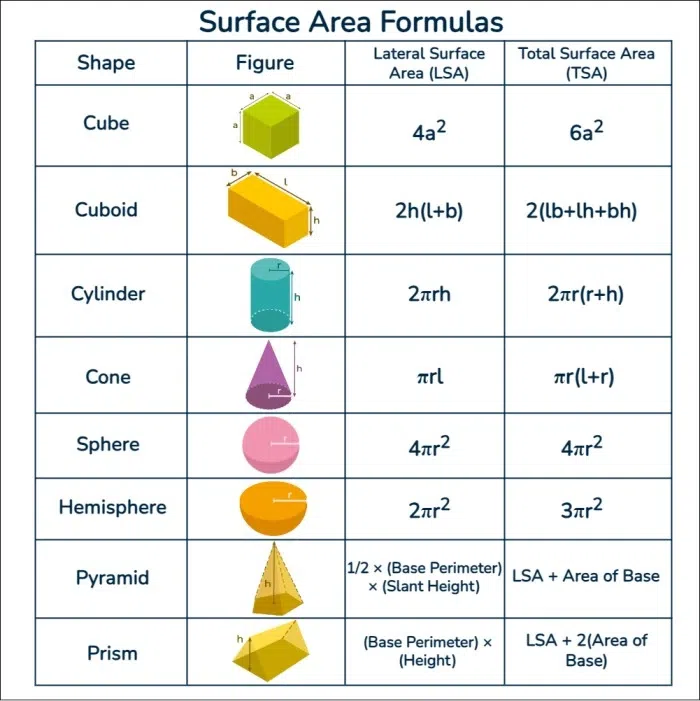
\includegraphics[width=0.8\textwidth]{imgs/Surface-Area-Formulas.png}
\end{minipage}
\end{center}
\newpage

\section{Unit 4 - Curve Sketching}
\subsection{Increasing and Decreasing Functions}
For a continuous and differentiable function, f, the function values(y-values) are increasing for all x-values where $f'(x)>0$, and the function values (y-values) are decreasing for all x-values where $f'(c)<0$
\subsubsection{Example 1a)}
Determine the intervals of increase and decrease for the function $$y=x^3+3x^2-2$$
\subsubsection*{Solution:}
\begin{align*}
    y&=3x^2+6x\\
    &=3(x+2)
\end{align*}
\begin{center}
 \begin{tikzpicture}[scale=1.5]
  % Draw axes
  \draw[->] (-3,0) -- (1.5,0) node[right] {$y'$};
  % Draw points
  \filldraw[black] (-2,0) circle (1pt) node[below] {$-2$};
  \filldraw[black] (0,0) circle (1pt) node[below] {$0$};
  
  % Draw plus and minus signs
  \node at (-2.5,0.3) {$+$};
  \node at (-1,0.3) {$-$};
  \node at (1,0.3) {$+$};
\end{tikzpicture}
\end{center}

$\therefore$ the intervals of increase are $x\in(-\infty,-2)\cup(0, \infty)$

$\therefore$ the intervals of decrease are $x\in (-2,0)$

\subsubsection{Example 1b)}
Determine the intervals of increase and decrease of the function $f(x)=\frac{x}{x^2+1}$
\subsubsection*{Solution:}
\begin{align*}
    f'(x)&=\frac{x^2+1(1)-(x)(2x)}{(x^2+1)^2}\\
    &=\frac{x^2+1-2x^2}{(x^2+1)^2}\\
    &=\frac{-x^2+1}{(x^2+1)^2}\\
    &=\frac{-(x^2-1)}{(x^2+1)}\\
    &=\frac{-(x-1)(x+1)}{(x^2+1)^2}
\end{align*}

$\therefore$ the intervals of increase are $x\in(-\infty,-1)\cup(1, \infty)$

$\therefore$ the intervals of decrease are $x\in (-1,1)$
\subsubsection{Example 2}
Given a graph of $y=f'(x)$, graph the curve $y=f(x)$

\begin{center}
\begin{tikzpicture}[scale=0.6]
  % Grid
  \draw[gray!50,very thin] (-2,-2) grid (5,5);
  \draw[thick,->] (-2,0) -- (5,0) node[right] {$x$};
  \draw[thick,->] (0,-2) -- (0,5) node[above] {$y$};
  
  % Plot of f'(x)
  \draw[blue,domain=-0.3:2.3,smooth,variable=\x] plot ({\x},{3*\x*\x - 6*\x + 2}) node[right] {$f'(x)$};
  
  % Fill between curve and x-axis
  \fill[pattern=north east lines,pattern color=gray!50,domain=0:2.26328,variable=\x] (0,0) -- plot ({\x},{3*\x*\x - 6*\x + 2}) -- (3.16228,0) -- cycle;
  
  % Plot of f(x)
  \draw[red,domain=-0.5:2.7,smooth,variable=\x] plot ({\x},{\x*\x*\x - 3*\x*\x + 2*\x + 1}) node[right] {$f(x)$};
\end{tikzpicture}
\end{center}
\subsubsection{Example 3}
Find the constants a, b and c such that the graph of $y=-x^3+ax^2+bx+c$ will decrease to the point (-6, -200) and increase to the point (2, 56) and then decrease thereafter.
\subsubsection*{Solution:}
\begin{align*}
    y'&=-3x^2+2ax+b\\
    f'(-6)=0 &\implies -3(-6)^2+2a(-6)+b=0\\
    &-108-12a+b=0\\
    b&=12a+108 \quad \circled{1}\\
    f'(2)=0 &\implies -3(2)^2+2a(2)+b=0\\
    b&=-4a+12 \quad \circled{2}\\
    12a+108&=-6a+12\\
    16a&=-96\\
    a&=-6\\
    b&=-4a+12\\
    &=-4(-6)+2\\
    b&=36
    y=-x^3-6x^2+36x+c\\
    &\textbf{sub } (-6,-200)\\
    -200&=-(-6)^3-6(-6)^2+36(-6)+c\\
    16&=c \quad \therefore a=-6, b=36, c=16
\end{align*}
\subsection{Critical Points, Local Maxima and Local Minima}
\subsubsection{First Derivative Test:}
If $f'(x)$ goes from positive to 0 to negative, then there is a local maximum at the point where $f'(x)=0$
\begin{center}
\begin{tikzpicture}[scale=1.5]
  % Draw function f'(x)
  \draw[blue, thick, domain=0.5:2.5, smooth, variable=\x] plot ({\x},{-0.6*(\x-1.5)^2 + 1.8}) node[right] {$f'(x)$};
  
  % Draw local maximum point
  \filldraw[red] (1.5,1.8) circle (1pt) node[above right] {Local Maximum};
\end{tikzpicture}
\end{center}

Similarly, if $f'(x)$ goes from positive to undefined to negative, and if $f(x)$ is defined at the point where $f'(x)$ is undefined, then there is a local maximum at the point where $f'(x)=0$

\begin{center}
\begin{tikzpicture}[scale=1,cap=round]
 \tikzset{axes/.style={}}
 % The graphic
\begin{scope}[style=axes]
\draw[->] (-.5,0) -- (3,0) node[below] {$x$};
\draw[->] (0,-.5)-- (0,3) node[left] {$y$};
\draw[thick] (0.25,0.4) to [out=10,in=-90]  (1.5,2.5)
 to [out=-90, in=175] (2.75,.4);
\draw[thin] (1.5,2.5) -- ++ (0.2,0.6) node[above]{$f'(a)$ does not exist};
\draw (1.5,0.2) -- (1.5,-0.2) node[below]{$a$};
\end{scope}
\end{tikzpicture}
\end{center}

If $f'(x)$ goes from negative to 0 to negative, then there is a local minimum at the point where $f'(x)=0$

\begin{center}
\begin{tikzpicture}[scale=1.5]
  % Draw function f'(x)
  \draw[blue, thick, domain=0.5:2.5, smooth, variable=\x] plot ({\x},{0.6*(\x-1.5)^2 + 1.8}) node[right] {$f'(x)$};
  
  % Draw local minimum point
  \filldraw[red] (1.5,1.8) circle (1pt) node[below left] {Local Minimum};
\end{tikzpicture}
\end{center}

Similarly, if $f'(x)$ goes from negative to undefined to positive, and if $f(x)$ is defined at the point where $f'(x)$ is undefined, then there is a local minimum at the point where $f'(x)=0$
\begin{center}
\begin{tikzpicture}[scale=1.2,cap=round]
  % Axes
  \draw[->] (-0.5,0) -- (3,0) node[below] {$x$};
  \draw[->] (0,-0.5)-- (0,3) node[left] {$y$};
  
  % Curve
  \draw[thick] (0.25,2.6) to[out=-10,in=90] (1.5,0.5) to[out=80,in=175] (2.75,2.6);
  
  % Point and label for local minimum
  \draw (1.5,0.2) -- (1.5,-0.2) node[below] {$a$};
  
  % Label for "f'(a) does not exist"
  \draw[thin] (1.5,0.5) -- ++ (0,0.7) node[above, left] {$f'(a)$ does not exist};
\end{tikzpicture}
\end{center}

If $f'(x)$ goes from positive to 0 positive, then there is neither a maximum nor a minimum.
\begin{center}
\begin{tikzpicture}[scale=1.5]
  % Draw axes
  \draw[->] (-2,0) -- (2,0) node[right] {$x$};
  \draw[->] (0,-2) -- (0,2) node[above] {$y$};
  
  % Plot of x^3
  \draw[blue, thick, domain=-1:1.1, smooth, variable=\x] plot ({\x},{\x*\x*\x}) node[right] {$f(x)=x^3$};
  
  % Label indicating positive slope
  \node[above right] at (1,2) {Positive slope};  
  % Label indicating positive slope again
  \node[below left] at (-1,-1) {Positive slope};
\end{tikzpicture}
\end{center}
If $f'(x)$ goes from negative to 0 negative, then there is neither a maximum nor a minimum.
\begin{center}
\begin{tikzpicture}[scale=1.5]
  % Draw axes
  \draw[->] (-2,0) -- (2,0) node[right] {$x$};
  \draw[->] (0,-2) -- (0,2) node[above] {$y$};
  
  % Plot of x^-3 (negative part)
 \draw[blue, thick, domain=-1:1.1, smooth, variable=\x] plot (-{\x},{\x*\x*\x}) node[left] {$f(x)=-x^3$};
  
  % Label indicating negative slope
  \node[above left] at (-1,2) {Negative slope};
  
  % Label indicating negative slope again
  \node[below right] at (1,-1) {Negative slope};
\end{tikzpicture}
\end{center}
\subsubsection{Critical Points and Critical Numbers}
The points at which $f(x)$ is defined and $f'(x)$ is undefined are called critical points.

The values of x at which $f'(x)=0$ or $f'(x)$ is undefined are called critical numbers.

\subsubsection{Example 1}
For function $y=x^4-8x^3+18x^2$, determine all critical points. Determine whether each of these values of x gives a local maximum or neither.
\subsubsection*{Solution:}
\begin{align*}
    y'=4x^3-24x^2+36x\\
    &=4x(x^2-6x+9)\\
    &=4x(x-3)^2
\end{align*}
Our critical numbers are $x=0$ and $x=3$\\
\begin{align*}
    &\text{at } x=0, y=(0)^4-8(0)^3+18(0)^2\\
    &(0,0)\\
    &\text{at } x=3, y=(3)^4-8(3)^3+18(3)^2\\
    &(3,27)
\end{align*}
$\therefore$ Our critical points are (0,0) which represents a minimum and (3,27) which represents neither a minimum nor a maximum.
\subsubsection{Example 2}
Determine whether the function $f(x)=x^3$ has a maximum or a minimum or neither at $(c, f(c))$ where $f'(c)=c.$
\subsubsection*{Solution}
\begin{align*}
    f'(x)&=3x^2\\
    3x^2=0 &\implies x=0\\
    \text{at } x=0,& y=(0)^3\\
    &=0\\
    &(0,0)
\end{align*}
$\therefore$ at (0,0) there is neither a maximum nor a minimum.

\newpage
\subsection{Asymptotes etc.}
\subsubsection{Testing for Vertical Asymptotes and Holes} 
Given a rational function of the form $$f(x)=\frac{p(x)}{q(x)},$$ we should simplify by crossing out like factors from the numerator and the denominator. 
\begin{enumerate}
    \item There is a hole at $x = c$ if the factor $(x –c)$ was originally present in both the numerator and the denominator and if the degree of that factor in the numerator was greater than or equal to the degree of that factor in the denominator. In other words, if $(x –c)$ is present in both the numerator and denominator and if, after simplifying, it is completely crossed out of the denominator, then there is a hole at  $x = c$. To determine the y-coordinate of the hole, plug the x-value into the simplified rational expression.
    \item There’s a vertical asymptote at $x = c$ if, AFTER SIMPLIFYING, the denominator equals 0 at $x = c$ and the numerator does not equal 0at $x = c$.
\end{enumerate}

\subsubsection{Test for Horizontal and Oblique Asymptotes}
Given a rational function of the form $$f(x)=\frac{p(x)}{q(x)},$$ we should simplify by crossing out like factors from the numerator and the denominator. If the denominator is degree 0 (i.e, there are no more x’s), then there are no horizontal or oblique asymptotes. If the denominator is not degree 0, then, AFTER SIMPLIFYING:
\begin{enumerate}
    \item There’s a horizontal asymptote at y = 0 if the degree of the denominator is greater than the degree of the numerator.
    \item There’s a horizontal asymptote at $$y=\frac{\text{lead coefficient of numerator}}{\text{lead coefficient of denominator}}$$ if the degree of the numerator equals the degree of the denominator. (Remember, the denominator must be at least degree 1 after simplifying)
    \item There’s an oblique asymptote if the degree of the numerator is greater than the degree of the denominator.  To determine the equation of the oblique asymptote, we use synthetic division or long division
\end{enumerate}
\subsubsection{Example 1}
Determine the equation of any asymptotes and the location of any holes(including y-coordinates) of the function $y=\frac{2x-2}{x^2+3x-4}$
\subsubsection*{Solution}
\begin{align*}
    &=\frac{2(x-1)}{(x+4)(x-1)}\\
    &=\frac{2}{(x+4)}\\
    &\text{hole at } x=1\\
    &\text{y-coordinate of hole: } \frac{2}{1+4}=\frac{2}{5}\\
    &\text{hole at } \left(1, \frac{2}{5}\right)\\
    &\text{V.A at } x=-4\\
    &\frac{\text{degree 1}}{\text{degree 2}} \implies \text{H.A at } y=0
\end{align*}
\subsubsection{Example 2}
Determine the equations of any asymptotes and the locations of any holes(including y-coordinate) of the function $y=\frac{5x+15}{2x+12}$
\subsubsection*{Solution}
\begin{align*}
    &y=\frac{5(x+3)}{2(x+6)}\\
    & \text{V.A at } x=-6\\
    & \text{H.A at } y=\frac{5}{2}
\end{align*}
\subsubsection{Example 3}
Determine the equations of any asymptotes and the locations of any holes(including y-coordinate) of the function $y=\frac{3x^2+15x-18}{4x^2-20x-24}$
\subsubsection*{Solution}
\begin{align*}
    &=\frac{3(x+6)(x-1)}{4(x-6)(x+1)}\\
    &\text{V.A at } x=6 \text{ and } x=-6\\
    &\text{H.A at } y=\frac{3}{4}
\end{align*}
\subsubsection{Example 4}
Determine the equation of any asymptotes and the location of any holes(including y-coordinate) of the function $y=\frac{x^2-2x+4}{x-3}$
\subsubsection*{Solution}
We cannot factor
$\therefore$ V.A at x=3\\
oblique (or slant) aspmptote 
$$\polyhornerscheme[x=3]{x^2-2x+4}$$
$$y=x+1+\frac{7}{x-3}$$
$$\therefore \text{O.A at } y=x+1$$
\subsubsection{Example 5}
Find constants a and b such that the graph of the function $y=\frac{ax+8}{bx-1}$ has a horizontal asymptote at $y=8$ and a vertical asymptote at $x=-5$
\subsubsection*{Solution}
\begin{align*}
    \text{V.A at } x=-5 \implies b(-5)-1&=0\\
    -5b-1&=0\\
    -5b&=1\\
    b&=-\frac{1}{5}\\
    \text{H.A at } y=8 \implies \frac{a}{b}&=8\\
    \frac{a}{-\frac{1}{5}}=8 \implies a &=-\frac{8}{5}\\
    \therefore a=-\frac{8}{5}, \quad b&=-\frac{1}{5}
\end{align*}
\newpage
\subsection{Concavity and Points of Inflection}
\subsubsection{Concave Up [$f''(x)>0$]}
\underline{Concave Up:} $f''(x)>0$. The graph of $y=f(x)$ is a concave up when the second derivative is positive. i.e when $f''(x)>0$.
\begin{figure}[ht]
    \centering
    \includegraphics[width=0.7\textwidth]{imgs/concave-up.png}
\end{figure}

Notice that the tangent lines go from a slope of negative to zero to positive. In other words the slopes are increasing meaning that the rate of change of the rate of change is positive(i.e $f''(x)>0$). When $f''(x)>0$, the curve is above the tangent lines. 

\subsubsection{Concave Down [$f''(x)<0$]}
\underline{Concave Down: } $f''(x)<0$. The graph of $y=f(x)$ is concave down when the second derivative is negative. i.e, when $f''(x)<0$.
\begin{figure}[ht]
    \centering
    \includegraphics[width=0.7\textwidth]{imgs/concave-down.png}
\end{figure}

Notice that the tangent lines go from a slope of positive,to zero, to negative. In other words, the slopes are decreasing, meaning that the rate of change of the rate of change is negative (i.e  $f''(x)<0$). When $f''(x)<0$, the curve is below the tangent lines.

\subsubsection{Second Derivative Test}
If at a given point, $f'(x)=0$ and $f''(x)=0$, then there is a local minimum.
\begin{figure}[ht]
    \centering
    \includegraphics[width=0.5\textwidth]{imgs/local-minimum.png}
\end{figure}

If at a given point, $f'(x)=0$ and $f''(x)<0$, then there is a local maximum.
\begin{figure}[ht]
    \centering
    \includegraphics[width=0.5\textwidth]{imgs/local-maximum.png}
\end{figure}

\subsubsection{Points of Inflections}
Points at which $f''(x)=0$ are called points of inflection.
\begin{figure}[ht]
    \centering
    \includegraphics[width=0.7\textwidth]{imgs/points_of_inflections.png}
\end{figure}
\newpage 
\subsubsection{Putting Together $f'(x)$ and $f''(x)$}

\begin{figure}[h]
    \centering
    \includegraphics[width=1\textwidth]{imgs/putting_together.png}
\end{figure}
\subsubsection{Key Ideas}
\textbf{Concavity:}
\begin{itemize}
    \item The graph of a function is concave up on an interval if it is increasing on the interval.
    \item The graph of a function is concave down on an interval if it is decreasing on the interval.
\end{itemize}

\textbf{Point of Inflection:}
\begin{itemize}
    \item A point of inflection is a point on the graph of a function where the function changes from concave up to concave down, or vice versa, or is undefined if it is a point of inflection on the graph.
\end{itemize}

\textbf{Need to Know:}
\begin{itemize}
    \item Test for concavity: If $f$ is a differentiable function whose second derivative exists on an open interval $I$, then
    \begin{itemize}
        \item the graph of $f$ is concave up on $I$ if $f''(x) > 0$ for all values of $x$ in $I$.
        \item the graph of $f$ is concave down on $I$ if $f''(x) < 0$ for all values of $x$ in $I$.
    \end{itemize}
    \item The second derivative test: Suppose that $f$ is a function for which $f'(c) = 0$ and the second derivative $f''(x)$ exists on an interval containing $c$.
    \begin{itemize}
        \item If $f''(c) > 0$, then $f$ has a local minimum value at $x = c$.
        \item If $f''(c) < 0$, then $f$ has a local maximum value at $x = c$.
        \item If $f''(c) = 0$, then the test fails. Use the first derivative test.
    \end{itemize}
\end{itemize}
\newpage
\subsection*{Example 1}
Sketch the graph of $y=x^3-3x^2-9x+10$
\subsection*{Solution}
\begin{align*}
    y' &= 3x - 6x - 9 \\
    &= 3(x^2 - 2x - 3) \\
    &= 3(x - 3)(x + 1) \\
    y' &= 3(x - 3)(x + 1) \\
    y' = 0 & \text{ at } x = 3 \text{ and } x = -1
\end{align*}
\begin{minipage}{0.5\linewidth}
At $x=-3$ 
\begin{align*}
    y&=3^3-3(3)^2-9(3)+10\\
    &=-17\\
    &(3,-17)
\end{align*}
\end{minipage}
\begin{minipage}{0.5\linewidth}
At $x=-1$ 
\begin{align*}
    y&=(-1)^3-3(-1)^2-9(-1)+10\\
    &=15\\
    &(-1,15)
\end{align*}
\end{minipage}
\begin{minipage}{0.5\linewidth}
\begin{align*}
    y'' &= 6x - 6 \\
    &= 6(x - 1) \\
    y'' &= 0 \quad \text{at } x = 1
\end{align*}
\end{minipage}
\begin{minipage}{0.5\linewidth}
\begin{align*}
\text{At } x &= 1 \\
y &= (1)^3 - 3(1)^2 - 9(1) + 10 \\
&= -1 \\
&(1, -1)
\end{align*}
\end{minipage}
\begin{figure}[h]
    \centering
    \begin{minipage}{0.5\textwidth}
        \centering
        \includegraphics[width=\textwidth]{imgs/alg 1.png}
        \caption{Intervals}
        \label{fig:alg1}
    \end{minipage}%
    \begin{minipage}{0.5\textwidth}
        \centering
        \includegraphics[width=\textwidth]{imgs/y=x^3-3x^2-9x+10.png}
        \caption{Graph of $y=x^3-3x^2-9x+10$}
        \label{fig:graph}
    \end{minipage}
\end{figure}
\newpage 
\subsection*{Example 2}
Sketch the graph of the function $f(x)=x^{\frac{1}{3}}$.
\subsubsection*{Solution}
\begin{align*}
    f'(x)&=\frac{1}{3}x^{-\frac{2}{3}} = \frac{1}{3x^{\frac{2}{3}}}\\
    f''(x)&=-\frac{2}{9}x^{\frac{-5}{3}}=\frac{1}{9x^{\frac{5}{3}}}
\end{align*}
\begin{itemize}
    \item $f'(x)$ never equal 0
    \item $f'(x)$ undefined at $x=0$ (0,0)
    \item $f''(x)$ never equal 0
    \item $f''(x)$ undefined at $x=0$ (0,0)
\end{itemize}
\begin{figure}[h]
    \centering
    \begin{minipage}{0.5\textwidth}
        \centering
        \includegraphics[width=\textwidth]{imgs/alg 2.png}
        \caption{Intervals}
        \label{fig:alg1}
    \end{minipage}%
    \begin{minipage}{0.5\textwidth}
        \centering
        \includegraphics[width=\textwidth]{imgs/y=x^1.png}
        \caption{Graph of $y=x^{\frac{1}{3}}$}
        \label{fig:graph}
    \end{minipage}
\end{figure}
\newpage 
\subsubsection*{Example 3}
Determine any points of inflection on the graph of $f(x)=\frac{1}{x^2+3}$.
\subsubsection*{Solution}
\textbf{First Derivative:}
\begin{align*}
f(x) &= \frac{1}{x^2+3} \\
f'(x) &= \frac{d}{dx} \left(\frac{1}{x^2+3}\right) \\
     &= \frac{0 \cdot (x^2+3) - 1 \cdot 2x}{(x^2+3)^2} \\
     &= \frac{-2x}{(x^2+3)^2}
\end{align*}

\textbf{Second Derivative:}
\begin{align*}
f'(x) &= \frac{-2x}{(x^2+3)^2} \\
f''(x) &= \frac{d}{dx} \left(\frac{-2x}{(x^2+3)^2}\right) \\
      &= \frac{-2(x^2+3)^2 - (-2x) \cdot 2(x^2+3)(2x)}{(x^2+3)^4} \\
      &= \frac{-2(x^4 + 6x^2 + 9) + 8x^2(x^2+3)}{(x^2+3)^4} \\
      &= \frac{-2x^4 - 12x^2 - 18 + 8x^4 + 24x^2}{(x^2+3)^4} \\
      &= \frac{6x^4 + 12x^2 - 18}{(x^2+3)^4}\\
      &=\frac{6(x-1)(x+1)}{(x^+3)^3}
\end{align*}
At $x=-1$
$$y=\frac{1}{(1)^+3}=\frac{1}{4} \quad \left(-1, \frac{1}{4}\right)$$
At $x=1$
$$y=\frac{1}{(-1)^+3}=\frac{1}{4} \quad \left(1, \frac{1}{4}\right)$$
$\therefore$ 2 points of inflection are $$\left(-1, \frac{1}{4}\right) \& \left(1, \frac{1}{4}\right)$$

\subsection{Graphing Curves}
\underline{Algorithm for Curve Sketching:}
\begin{enumerate}
    \item Determine $y$-intercept if it exists (let $x=0$)
    \item Determine $x$-intercepts if they exist (let $y=0$)
    \item Determine any holes (including $y$-coordinate) or vertical asymptotes
    \item Determine any horizontal or oblique asymptotes
    \item Determine intervals of increase and decrease (determine $x$-values at which $y'$ is zero or undefined and do interval testing)
    \item Determine intervals of concavity (determine $x$-values at which $y''$ is zero or undefined and do interval testing)
    \item "Stack" the intervals created in numbers 5 and 6
    \item Determine the associated $y$-values of any points where $y'$ or $y''$ is zero or undefined and graph those points
    \item Don't forget what you already know about graphs \smiley{} 
\end{enumerate}

For the following diagrams, assume that the function is defined all the way through the interval.
\begin{figure}[ht]
    \centering
    \begin{subfigure}[b]{0.9\textwidth}
        \centering
        \includegraphics[width=\linewidth]{imgs/diagram_1_2.png}
        \caption{}
    \end{subfigure}
    
    \begin{subfigure}[b]{0.45\textwidth}
        \centering
        \includegraphics[width=\linewidth]{imgs/diagram_3.png}
        \caption{}
    \end{subfigure}
    \hfill
    \begin{subfigure}[b]{0.45\textwidth}
        \centering
        \includegraphics[width=\linewidth]{imgs/diagram_4.png}
        \caption{}
    \end{subfigure}
    
    \begin{subfigure}[b]{0.9\textwidth}
        \centering
        \includegraphics[width=\linewidth]{imgs/diagram_5_6.png}
        \caption{}
    \end{subfigure}
    
    \begin{subfigure}[b]{0.9\textwidth}
        \centering
        \includegraphics[width=\linewidth]{imgs/diagram_7_8.png}
        \caption{}
    \end{subfigure}
    
    \caption{All diagrams}
\end{figure}

\clearpage % New page

\section{Unit 5 - Derivatives of Exponential and Trigonometric Functions}
\subsection{Trig Derivatives}
The two main rules to remember are the following:
\begin{tcolorbox}[sharp corners=uphill,
    colback=purple!50!white,colframe=blue!25!black,coltext=yellow,
    fontupper=\Large\bfseries,arc=6mm,boxrule=2mm,boxsep=5mm]
    $$\frac{\delta (\sin x)}{\delta x}=\cos x \quad \text{and } \quad \frac{\delta(\cos x)}{\delta x}=-\sin x$$
\end{tcolorbox}

\textit{Proof} that $\frac{\delta (\sin \theta)}{\delta x}=\cos \theta$.\\
We will do this proof in two parts. 


In the first part, we will prove that  $\lim_{\theta \to 0}\left( \frac{\sin \theta }{\theta}\right)$\\

We need to prove this because it comes up within the main proof, which we will then do in part 2.\\

Part 1: Proving that $\lim_{\theta \to 0}\left( \frac{\sin \theta }{\theta}\right)$\\

Recall that the area of a circle is $\pi r^2=(\frac{2 \pi}{2})r^2$ \\
We will think of our angle $\theta$ in radians \\
The area of the sector of a circle created by a central angle of $\theta$ radians will represent $\frac{\theta}{2\pi}$ of the area of the circle as a whole \\

\begin{minipage}{0.5\textwidth}
For example, if the angle shown is $60^{\circ}$, or $\frac{\pi}{3}$ radians, then the area of the highlighted sector will represent $\left(\frac{\frac{\pi}{3}}{2\pi}\right)=\frac{\pi}{3}\times \frac{1}{2\pi}=\frac{\pi}{6\pi}=\frac{1}{6}$ of the area of the circle as a whole.
\end{minipage}
\hspace{1em}
\begin{minipage}{0.5\textwidth}
\begin{tikzpicture}[scale=2.5] 
\draw (0,0) circle (1cm);
\draw (0,0) -- (0:1cm); 
\draw (0,0) -- (60:1cm); 

\draw (0.2,0) arc (0:60:0.2cm); 
\node at (0.3,0.1) {$\theta$};
\end{tikzpicture}
\end{minipage}

\hspace{1em}


Therefore, for a circle with a radius of r, the area of a sector of that circle created by central angle of $\theta$ radians is given formula \\

\begin{align*}
    \text{Area of Sector} &= \left(\frac{\theta}{2 \oi}\right )(\text{area of circle})\\
    &=\left(\frac{\theta}{2 \pi}\right)(\pi ^2)\\
    &=\left(\frac{\theta}{2}\right)r^2
\end{align*}


Now, focusing on Sector OAB, the length of OB is the radius of the circle from which Sector OAB originates. B and C share the same x-coordinate, as C lies on a vertical line from B. Since C is outside the unit circle, its x-coordinate must be $\cos \theta$. Thus, the radius of the circle from which Sector OAB originates is $\cos \theta$.

As previously stated, the area of a sector is $\left(\frac{\theta}{2}\right)r^2$, and since $r=\cos \theta$, the area of Sector OAB is $\left(\frac{\theta}{2}\right)\cos^2\theta$.

Now, let’s consider Triangle OCB. Its area is $\frac{1}{2}bh$. The base of the triangle is $\cos \theta$, and the height is the y-coordinate of C, which is $\sin \theta$. Thus, the area of Triangle OCB is $\frac{1}{2}\cos \theta \sin \theta$.

Moving to Sector OCD, the area of a sector is $\left(\frac{\theta}{2}\right)r^2$. Since the radius of this sector is 1 (from a unit circle), the area of Sector OCD is $\left(\frac{\theta}{2}\right)(1)^2 = \frac{\theta}{2}$.

Therefore, we have:
\begin{align*}
    &\text{area of Sector OAB is equal to } \left(\frac{\theta}{2} \right)\cos^2\theta\\
    &\text{area of Triangle OCB is } \frac{1}{2}\cos \theta \sin \theta \\
    &\text{area of Sector OCD is } \frac{\theta}{2}
\end{align*}


Putting together the statement above and the statement to the right, we get
\begin{equation*}
    \left(\frac{\theta}{2} \right)\cos^2\theta \leq \frac{1}{2}\cos \theta \sin \theta \leq \frac{\theta}{2}
\end{equation*}

Next, we multiplying the left middle and right by $\frac{2}{\theta \cos \theta}$ gives us 
$$
    \left(\frac{\theta}{2}\right) \cos ^2 \theta \left[\frac{2}{\theta \cos \theta}\right] \leq \frac{1}{2}\cos \theta \sin \theta \left[\frac{2}{\theta \cos \theta}\right] \leq \frac{\theta}{2} \left[\frac{2}{\theta \cos \theta}\right]
$$
$$\cos \theta \leq \frac{\sin \theta}{\theta} \leq \frac{1}{\cos \theta}$$

Determine the limit as $\theta \to 0$ of the left, middle and right
$$\lim_{\theta \to 0}\cos \theta \leq \lim_{\theta \to 0}\frac{\sin \theta}{\theta} \leq \lim_{\theta \to 0}\frac{1}{\cos \theta}$$
We can evaluate the left and the right be simply subbing in a value of $\theta=0$ because those functions are continuous in the neighbourhood around $\theta=0$

\begin{align*}
   & \cos 0 \leq \lim_{\theta \to 0} \frac{\sin \theta}{\theta} \leq \frac{1}{\cos \theta}\\
   & 1 \leq \lim_{\theta \to 0} \frac{\sin \theta}{\theta} \leq \frac{1}{1}\\
   & 1 \leq \lim_{\theta \to 0} \frac{\sin \theta}{\theta} \leq 1
\end{align*}
This next part is really cool, why?\\
The only way that 1 can be both less than or equal to a particular quantity and that the same quantity is less than or equal to 1 is if that quantity is equal to 1.\\
In other words, that quantity is being squeezed so that it’s only possible value is 1

$$\therefore \lim_{\theta \to 0}\frac{\sin \theta}{\theta}=1$$
Part 2:  We needed that result because there will be a moment in our proof that $$\frac{\delta(\sin \theta)}{\delta \theta}=\cos \theta$$ where that value comes up.
\begin{align*}
    \frac{\delta (\sin \theta)}{\delta \theta}&=\lim_{h \to 0}\frac{\sin(\theta+h)-\sin \theta}{h} \text{(next, use compound angle formula)}\\
    &=\lim_{h\to 0}\frac{\sin \theta \cos (h)+\cos \theta \sin(h)-\sin \theta}{h} \text{(next, rearrange the numerator)}\\
    &= \lim_{h\to 0}\frac{\sin \theta \coh (h)-\sin \theta +\cos \theta \sin(h)}{h} \text{(next, split into two fractions)}\\ 
    &=\lim_{h \to 0} \frac{\sin \theta \cos(h)-\sin \theta }{h}+\frac{\cos \theta \sin \theta \sin(h)}{h} \text{(next, factor each numerator)}\\
    &=\lim_{h \to 0} \frac{\sin \theta []\cos (h)-1}{h}+\cos \theta \left(\frac{\sin (h)}{h}\right)\\
    &=\lim_{h \to 0} \sin \theta \left[\frac{\cos (h)-1}{h}\right]+ \cos \theta \left(\frac{\sin (h)}{h}\right)\\    
    &\text{Evaluate the sum of the limits rather than the limit of the sum}\\
    &=\lim_{h \to 0} \sin \theta \left[\frac{\cos (h)-1}{h}\right]+ \lim_{h \to 0}\cos \theta \left(\frac{\sin (h)}{h}\right)\\    
\end{align*}

\newpage 
We can pull $\sin \theta$  in front of the first limit since it’s independent of h and we can pull $\cos \theta$ in front of second limit since it’s also independent of h
$$
\begin{aligned}
& =\sin \theta \lim _{h \rightarrow 0} \frac{\cos (h)-1}{h}+\cos \theta \lim _{h \rightarrow 0} \frac{\sin (h)}{h} \\
& =\sin \theta \lim _{h \rightarrow 0}\left(\frac{\cos (h)-1}{h}\right)\left(\frac{\cos (h)+1}{\cos (h)+1}\right)+\cos \theta \\
& =\sin \theta \lim _{h \rightarrow 0}\left[\frac{\cos ^2 h-1}{h[\cos (h)+1]}\right]+\cos \theta \\
& =\sin \theta \lim _{h \rightarrow 0} \frac{-\sin ^2 h}{h[\cos (h)+1]}+\cos \theta
\end{aligned}
$$
Next, we’ll break apart the fraction of which we are taking the limit:
$$
\begin{aligned}
& =\sin \theta\left[\lim _{h \rightarrow 0}\left(\frac{-\sin (h)}{h} \times \frac{\sin (h)}{\cos (h)+1}\right)\right]+\cos \theta \\
& =\sin \theta\left[\lim _{h \rightarrow 0} \frac{-\sin h}{h} \times \lim _{h \rightarrow 0} \frac{\sin (h)}{\cos (h)+1}\right]+\cos \theta \\
& =\sin \theta\left[-\lim _{h \rightarrow 0} \frac{\sin (h)}{h} \times \lim _{h \rightarrow 0} \frac{\sin (h)}{\cos (h)+1}\right]+\cos \theta \\
& =\sin \theta\left[-(1) \times \frac{\sin 0}{\cos 0+1}\right]+\cos \theta \\
& =\sin \theta\left[-1 \times \frac{0}{1+1}\right]+\cos \theta \\
& =\sin \theta[-1 \times 0]+\cos \theta
\end{aligned}
$$
Consider the product of the limits rather than the limit of the product:
\begin{align*}
    &=\sin[-1\times 0]+\cos\theta\\
    &=(\sin\theta)(0)+\cos \theta\\
    &=\cos \theta
\end{align*}
Therefore, $\frac{\delta (\sin \theta)}{\delta \theta}=\cos \theta$ QED.

\newpage 
\begin{tcolorbox}[colback=Orchid!5!snow, colframe=nadeshikopink!50!white,
  colbacktitle=mordantred19!75!mistyrose, title=Trigonometric Identities ]
$$
\begin{aligned}
& \sin (a+b)=\sin a \cos b+\cos a \sin b \\
& \sin (a-b)=\sin a \cos b-\cos a \sin b \\
& \cos (a+b)=\cos a \cos b-\sin a \sin b \\
& \cos (a-b)=\cos a \cos b+\sin a \sin b \\
& \sin 2 x=2 \sin x \cos x \\
& \cos 2 x=\cos ^2 x-\sin ^2 x \\
& =1-2 \sin ^2 x \text {. } \\
& =2 \cos ^2 x-1 \\
& \lim _{x \rightarrow 0} \frac{\sin x}{x}=1 \\
&
\end{aligned}
$$
Make sure you remember all these identities, you don't need to memorize it :)
\end{tcolorbox}

\subsubsection*{Examples}
Determine the derivatives of each of the following with respect to x:
\begin{enumerate}
    \item[a)] $y=\cos x$\\ 
    \textbf{Solution:}\\
    This is just a straightforward application of the second main rule above
    $$y'=-\sin x$$
    \item[b)] $y=x \sin x$\\
    \textbf{Solution:}\\
    This is a product rule situation
    \begin{align*}
        y'&=(1)\sin + x(\cos x)\\
        y'&=\sin x + x\cos x
    \end{align*}
    \item[c)] $y=\sin x^2$\\
    \textbf{Solution:} In this case, the exponent of 2 is operating only on x, not sin x\\
    This is a chain rule situation; the derivative of sin block is cos block times the derivative of the block \\
    Therefore, $y'=\cos x^2(2x)$\\
    Now, it is important to know that the 2x does not multiply $x^2$, but rather it multiplies the whole quantity (i.e., the 2x multiplies $\cos x^2$\\
    Therefore, $y'=2x\cos x^2$\\

\end{enumerate}

\subsection{Trig Optimization Word Problems Part 1}
\subsubsection*{Example 1:}
A thin rigid pole is carried around a 90 degree angle. The hallways are 1.2 metres wide at 1.6 metres wide. What is the longest possible pole? No domain is necessary.


\begin{minipage}{0.5\textwidth}
  \centering
  \includegraphics[width=\textwidth]{imgs/op1.png}
\end{minipage}%
\begin{minipage}{0.5\textwidth}
\begin{align*}
    L &= \ell_1 + \ell_2 \\
    L(\theta) &= \frac{1.2}{\sin \theta} + \frac{1.6}{\sin \theta} \\
              &= 1.2(\sin \theta)^{-1} + 1.6(\cos \theta)^{-1} \\
    L'(\theta) &= 1.2(\sin \theta)^{-2} + 1.6(\cos \theta)^{-2} \\
    L'(\theta) &= 0 \implies \textcolor{red}{-1.2(\sin \theta)^{-2}(\cos \theta)} - \textcolor{blue}{1.6(\cos \theta)^{-2}(-\sin \theta)} \\
\end{align*}
\end{minipage}

\begin{align*}
    & \textcolor{red}{\underbrace{\frac{-1.2(\cos \theta )}{(\sin \theta)^2}}} + \textcolor{blue}{\underbrace{\frac{1.6 \cos \theta }{(\cos \theta)^2}}} = 0 \\
    & \frac{1.6 \cos \theta }{(\cos \theta)^2} = \frac{1.2(\cos \theta )}{(\sin \theta)^2} \\
    & 1.6 \sin^3\theta = 1.2 \cos ^3 \theta \\
    & \frac{1.6 \sin^3 \theta}{\cos ^3\theta} = 1.2 \\
    & \frac{\sin^3 \theta}{\cos ^3\theta} = \frac{1.2}{1.6} \\
    & \left(\frac{\sin \theta }{\cos \theta}\right)^3 = \frac{1.2}{1.6} \\
    & (\tan)^3 = \sqrt[3]{\frac{1.2}{1.6}} \\
    & \theta \approx 42.26^{\circ}
\end{align*}
\[
L(42.26) = \frac{1.2}{\sin 42.26^{\circ}} \approx 3.95. \quad \therefore \text{max length is 3.95m.}
\]
\newpage
\subsubsection*{Example 2:}
Joey needs a ladder to break out of prison. He will lean the ladder against a tall fence, over the top of a 5 m high wall that is 3 m from the tall fence. He hopes to climb diagonally along the ladder, over the wall, to the fence. Then he climbs up and over the fence and escapes.\\
What is the minimum length of ladder necessary? No domain is necessary? 


\begin{minipage}{0.5\textwidth}
  \centering
  \includegraphics[width=\textwidth]{imgs/op2.png}
\end{minipage}%
\begin{minipage}{0.5\textwidth}
    \begin{align*}
        &L=\ell_1+\ell_2\\
        &L(\theta)=3(\cos\theta)^{-1}+5(\sin \theta)^{-1}\\
        &L'(\theta)=0 \implies \textcolor{red}{-3(\cos\theta)^{-2}(-\sin\theta)}-\textcolor{blue}{5(\sin \theta)^{-2}(\cos \theta)=0}
    \end{align*}
\end{minipage}
\begin{align*}
    &\frac{3\sin\theta}{\cos^2\theta}-\frac{-5\cos \theta}{\sin^2\theta}=0\\
    &\frac{3\sin \theta}{\cos^2\theta}=\frac{5\cos \theta}{\sin^2\theta}\\
    &3\sin^3\theta=5\cos^3\theta\\
    &\frac{\sin^3\theta}{\cos^3\theta}=\frac{5}{3}\\
    &\tan^3=\frac{5}{3}\\
    &\tan^3=\sqrt[3]{\frac{5}{3}}\\
    &\theta \approx49.85^{\circ}\\
\end{align*}
$$L(49.85^{\circ})=\frac{3}{\cos(49.85)}+\frac{5}{\sin(49.85)}\approx 11.2. \therefore \text{laddin must be at least 11.2m long} $$
\newpage 
\subsection{Trig Optimization Word Problem 2}
\subsubsection*{Example 1: }
Determine the greatest possible area of the trapezoid shown below; you are given three side lengths and the top side is as long as you need it to be.

\begin{minipage}{0.5\textwidth}
  \centering
  \includegraphics[width=\textwidth]{imgs/op3.png}
\end{minipage}%
\begin{minipage}{0.7\textwidth}
    \begin{align*}
        &\text{Area = }\text{(Area of $\Delta$)}(2)+ \ell \omega\\
        &\sin \theta=\frac{h}{2} \quad \cos \theta= \frac{\ell}{2}\\
        &h=\frac{2}{\sin\theta} \quad \boxed{\ell=2\cos\theta}\\
        &\boxed{h=2\sin\theta}
    \end{align*}
\end{minipage}
\begin{align*}
    &=\frac{1}{2}\left[2(\cos\theta)(2\sin\theta)(2)+3(2\sin\theta)\right]\\
    &A(\theta)=4\sin \theta\cos\theta+6\sin\theta\\
    &A'(\theta)=4\cos\theta\cos \theta + 4 \sin \theta(-\sin \theta)+6\cos \theta\\
    &A'(\theta)=0 \implies 4\cos^2 \theta -4\sin^2 \theta +6 \cos \theta=0\\
    &4 \cos^2-4(1-\cos ^2\theta)+6\cos \theta=0\\
    &4\cos^2\theta-4+4\cos^2\theta+6\cos \theta=0\\
    &8\cos^2\theta+6\cos -4=0\\
    &\cos \theta=\frac{=6\pm \sqrt{36+128}}{16}\\
    &0.425 \quad \text{or} \quad \cancel{-1.1753}\\
    &\cos^{-1}(0.425)\approx 64.8^{\circ}\\
\end{align*}
$$A(64.8^{\circ})=4\sin(64.8^{\circ})\cos(64.8^{\circ})+6\sin(64.8^{\circ})\approx6.97$$
\subsection{Derivatives of Exponential Functions}
Three key rules for this section are\\
\begin{itemize}
    \item The derivative of $\lm x$ with respect to $x$ is $\frac{1}{x}$
    \item The derivative of $e^x$ with respect to $x$ is $e^x$
    \item The derivative of $b^x$ with respect to $x$ is $(b^x)(\ln b)$
\end{itemize}

Putting the last rule together with the chain rule, we get that
$$\text{Derivative of } b^{f(x)} \text{is } b^{f(x)}(\ln n)f'(x)$$
\begin{tcolorbox}[colback=blue!5!snow, colframe=white!50!white,
  colbacktitle=blue!75!mistyrose, title=Derivatives of Exponential Functions Rules]
    \begin{align*}
        \frac{\delta(\ln x)}{\delta x}&=\frac{1}{x}\\
        \frac{\delta(e^x)}{\delta x}&=e^x\\
        \frac{\delta (b^x)}{\deleta x}&= b^{x}(\ln b)\\
        \frac{\delta (b^{f(x)})}{\delta x}&=b^{f(x)}\ln b f'(x)\\
    \end{align*}  
\end{tcolorbox}
In other words, to differentiate an exponential function, restate the function, multiply by the natural logarithm (ln) of the base, and then multiply by the derivative of the exponent. This is assuming that there is no $x$ in the base as well. We will see that there is a different process when there is an $x$ in both the base and in the exponent.

\subsubsection*{Example 1:}
Determine the derivative of $g(x)=e^{x^2-x}$
\subsubsection*{Solution: }
$g'(x)=e^{x^2-x}(2x-1)$
\subsubsection*{Example 2:}
Determine the derivative of the curve $f(x)=x^2e^x$
\subsubsection*{Solution:}
$f'(x)=2xe^e+x^2e^x$
\subsubsection*{Example 3:}
Determine the equation of the tangent line to $y=\frac{e^x}{x^2}$ where $x=1$.
\subsubsection*{Solution: }
at $x=1$, $y=\frac{e^1}{(1)^2}=\frac{e}{1} \quad (1, e)$ this is called the points.\\
The slope is:
$$y'=\frac{x^2e^x-e^x(2x)}{x^4}$$
$\therefore \text{at } x=1, y'=\frac{(1)^2e^1(2(1))}{(1)^4}= \frac{e-2e}{1}=-e$ \\
The question is not over yet, we need to solve the tangent of equation by using some skills from grade 9th math. Therefore:
\begin{align*}
    y&=mx+b\\
    y&=-ex+b\\
    &\text{plug in (1, e)}\\
    e&=-e(1)+b\\
    2e&=b
\end{align*}
$\therefore$ the equation of the tangent line is $y=-ex+2e$
\subsubsection*{Example 4:}
Differentiate the function $f(x)=5x^x$
\subsubsection*{Solution: }
$f'(x)=5^x(\ln 5)$
\subsubsection*{Example 5:}
Differentiate the function $h(x)=(8)7^{9x^2-5x+1}$
\subsubsection*{Solution: }
$h'(x)=(8)7^{9x^2-5x+1}(\ln 7)(18x-5)$

\subsubsection*{Word Problem 1:}
On January 1, 1850, the population of Goldrushtown was 50000. Since then the population of Goldrushtown can be expressed as $P(x)=50000(0.98)^t$.
\begin{enumerate}
    \item[a)] What was the population of Goldrushtown on January 1, 1900?
    \item{b)} At what rate was the population changing on January 1, 1900? 
\end{enumerate}
\subsubsection*{Solution: }
\begin{enumerate}
    \item[a)] $P(50)=50000(0.98)^{50} \approx 18208$
    \item[b)] 
    \begin{align*}
        P(x)&=50000(0.98)^t\\
        P'(x)&=50000(0.98)^t(\ln 0.98)\\
        P'(50)&=50000(0.98)^{50}(\ln 0.98)\\
        &\approx-367.8 = -368
    \end{align*} 
$\therefore$ the population is decreasing at rate of approximately 368 people per year.    
\end{enumerate}
\subsubsection*{Word Problem 2:}
A radioactive substance decays exponentially. The percent, P, of the material left after after t years is $P(t)=100(1.015)^{-t}$
\begin{enumerate}
    \item[a)] What is the half-life?
    \item[b)] How fast is the substance decaying at that time?
\end{enumerate}
\subsubsection*{Solution: }
\begin{enumerate}
    \item[a)]
    \begin{align*}
        50 &= 100 \times (1.015)^{-t}\\
        \frac{50}{100} &= (1.015)^{-t}\\
        \frac{1}{2} &= (1.015)^{-t}\\
        -t &= \log_{1.015}\left(\frac{1}{2}\right)\\
        -t &= \frac{\log\left(\frac{1}{2}\right)}{\log(1.015)}\\
        t &\approx 46.59
    \end{align*}
    $\therefore$ the lalf-life is approximately 47 years.
    \item[b)] 
    \begin{align*}
        P'(x)&=100(1.015)^{-t}\ln (1.015)\\
        P'(47)&=100(1.015)^{-47}\ln (1.015)\\
        &\approx 0.74
    \end{align*} 
    $\therefore$ at that time, the population is decreasing at the rate of 0.76\% of the original amount per year.
\end{enumerate}
\newpage 
\subsection{Optimization Involving Exponential Functions}
\subsubsection*{Example 1:}
The effectiveness of studying for an exam depends on how many hours a student studies. Some experiments show that if the effectiveness, E is put on a scale from 0 to 10, then
$$E(t)=0.5\left[10+te^{\frac{-t}{20}}\right]$$
where t is the number of hours spent studying for an examination. If a student has up to 30 hours for studying, how many hours are needed for maximum effectiveness?
\begin{align*}
    &=5+0.5t^{\frac{-t}{20}}\\
    E(t)=0 \implies & 0.5e^{-\frac{1}{20}t}+0.5te^{-\frac{1}{20}} \left(-\frac{1}{20}\right)=0\\
    &\underbrace{0.5e^{-\frac{1}{20}t}}_{\text{cannot equal to 0}} \underbrace{\left(1-\frac{1}{20}t\right)}_{\downarrow }=0\\
    &\quad \quad 1-\frac{1}{20}t=0 \implies 1=\frac{1}{20}t\\
    &\quad \quad \quad 20=t
\end{align*}
Now, we need to use the domain analysis:

\begin{align*}
    E(0)&=5+0.5(0)e^{-\frac{1}{20}}=5\\
    E(20)&\approx8.68\\
    E(30)&\approx8.35
\end{align*}
$\therefore$ the maximum effectiveness satvik should study 20 hours.
\newpage 

\subsubsection*{Example 2:}
A consultant determines that the proportion of people who have responded to the advertisement of a new product after it has been marketed for t days is given by $f(t)=0.7(1-e^{-0.2t})$.The area covered by that advertisement contains 10 million potential customers and each response to the ad yields revenue of \$0.70 on average (excluding the cost of advertising). The ad costs \$30000 to produce and a further \$5000 per day to run.

\begin{enumerate}
    \item[a)] Determine $\lim_{t\to\infty}f(t)$ and interpret the result.
    \item[b)] What percent of potential customers have responded after 7 days of advertising?
    \item[c)] Write the function P(t) that represents the average profit after t days of advertising. What is the average profit after 7 days?
    \item[d)] For how manyfull days should the ad campaign be run in order to maximize the average profit? Assume an advertising budget of \$200000.
\end{enumerate}
\subsubsection*{Solution: }
\begin{enumerate}
    \item[a)] 
    \begin{align*}
        &0.7-0.7e^{-0.2t}\\
        \lim_{t\to \infty}f(t) &=\lim_{t\to \infty}0.7-\frac{0.7}{e^{0.2t}}\\
        &=0.7
    \end{align*}
$\therefore$ if the ad runs forever, only 7070 of people will respond. 
    \item[b)] $f(7)=0.7-0.7e^{-0.2(7)}\approx 53$
    $\therefore$ after 7 days 539 of population have responded.
    \item[c)] 
    \begin{align*}
    \text{Profit } &= \text{Revenue - Cost}\\    
    \text{Revenue }&=(0.70)\text{(number of responses)}\\
    &=(0.70)\text{(population)(percentage of population who have responded)} \\
    &=(0.70)(1000000)(f(t))\\
    &=70000000\left[(0.7(1-e^{-0.2t}))\right]\\
    &=70000000(0.7-0.7e^{-0.2t})\\
    &=4900000-4900000e^{-0.2t}\\
    \end{align*}
    \begin{align*}
    \text{Cost} &= \text{Production cost + Opening cost}\\
    &=3000+5000\text{(\# of days)}\\
    c(t)&=30000+5000t\\
    P(t)&=R(t)-C(t)\\
    &=4900000-4900000e^{-0.2t}-(30000+5000t)\\
    &=4870000-4900000e^{-0.2t}-500t\\
    P(7)&=4870000-490000e^{-0.2(7)}-5000(7)\\
    &\approx 3626674.88
    \end{align*}
    \item[d)] 
    \begin{align*}
        \text{Domain Work}\\
        t &\geq 0\\
        \text{Cost} &\leq 200000\\
        300000+5000+&\leq 20000\\
        5000t&\leq 170000\\
        t&\geq34\\
        \therefore 0\leq &t \leq 34
    \end{align*} 
    \begin{align*}
        P'(t) 0\implies -4900000e^{-0.2t}(-0.2)-5000&=0\\
        98000e^{-0.2t}&=5000\\
        e^{-0.2t}&=\frac{5000}{98000}\\
        -0.2t&=\ln \left(\frac{5000}{980000}\right)\\
        t&=\frac{\ln \left(\frac{5000}{980000}\right)}{-0.2} \approx 26
    \end{align*}
    \begin{align*}
        P(0)&=487000-4900000e^{-0.2}-5000(0)=-30000\\
        P(26)&=4712968.83\\
        P(34)&=4694542.50
    \end{align*}
    $\therefore$ max profit at 26 days
\end{enumerate}
\newpage 
\subsection{Logarithmic Differentiation}
We know how to find the derivative of a power of x. For example, if we are given the function $y=3x^2$, we see that x is in the base of the exponent and we know that we can use the power rule.\\
We also know how to find the derivative of an exponential function, where x is in the exponent. For example, if we are given the function $y=3^{2x-1}$, we see that x is in the exponent and we can use exponential differentiation.\\
But what do we do if we have a function where x is in the base of the exponent and in the exponent. For example, how would we determine the derivative of the function $y=x^x$. \\
If we have a power with x in both the base of the exponent and in the exponent itself, we can determine the derivative by taking the natural logarithm (i.e., ln) of both sides, then using previously learned rules of derivatives such as implicit differentiation and the power rule, among others, to isolate $y'$ and thus determine the derivative

\subsubsection*{Example 1:}
Determine the derivative with respect to x of $y=x^x$.
\subsubsection*{Solution: }
\begin{align*}
    \log &= \ln x^x\\
    \ln y &=x\ln x\\
    \frac{1}{y} \frac{\delta y}{\delta x} &=\ln x +x\left(\frac{1}{x}\right)\\
    \frac{1}{y} \frac{\delta y}{\delta x} &=\ln x+1\\
    \frac{\delta y}{\delta x}&=x^x(\ln x+1)
\end{align*}
\subsubsection*{Example 2:}
Determine the derivative with respect to x of $y=(3x+4)^{x^4-2x}$
\subsubsection*{Solution: }
\begin{align*}
    \ln y &=\ln (3x+4)^{x^4-2x}\\
    \ln y &=(x^4-2x) \ln(3x+4)\\
    \frac{1}{y}\frac{\delta y}{\delta x}&=(4x^3-2)\ln(3x+4)+(x^4-2x)\left(\frac{1}{3x+4}\right)(3)   
\end{align*}
    \text{or}
    \begin{align*}
    \frac{\delta y}{\delta x}&=y\left[(4x^3-2)\ln(3x+4)+\frac{(x^4-2x)(3)}{3x+4}\right]\\
    \frac{\delta y}{\delta x}&=(3x+4)^{x^4-2x}\left[(4x^3-2)\ln(3x+4)+\frac{(x^4-2x)(3)}{3x+4}\right]\\ 
    \end{align*}
    Sometimes Logarithmic differentiation can be used to answer other questions where it might not necessarily be applicable.
    We will prove the power rule using Logarithmic differentiation in a moment, and then we will do an example where Logarithmic differentiation is beneficial to a question that would otherwise be rather complicated.
\subsubsection*{Example 3:}
    Using logarithmic differentiation, prove the power rule; i.e prove that if $f(x)=x^n$, then $f'(x)=nx^{n-1}$
\subsubsection*{Solution: }

First, take the natural logarithm of both sides:

$$\ln(f(x)) = \ln(x^n)$$

Using the property of logarithms that allows us to bring the exponent down as a coefficient, we get:

$$\ln(f(x)) = n \cdot \ln(x)$$

Now, differentiate both sides with respect to $x$. On the left side, we use the chain rule, and on the right side, the derivative of $\ln(x)$:

$$\frac{1}{f(x)} \cdot f'(x) = n \cdot \frac{1}{x}$$

Solving for $f'(x)$ gives us:

$$f'(x) = f(x) \cdot n \cdot \frac{1}{x}$$

Since $f(x) = x^n$, we substitute $f(x)$ back in:

$$f'(x) = x^n \cdot n \cdot \frac{1}{x}$$

Simplify the expression by canceling one $x$ from $x^n$ and $x$ in the denominator:

$$f'(x) = n \cdot x^{n-1}$$

And there we have it, the power rule is proven using logarithmic differentiation:

$$f'(x) = nx^{n-1}$$

This shows that the derivative of $x^n$ with respect to $x$ is indeed $nx^{n-1}$.

\subsubsection*{Example 4:}
Use logarithmic differentiation to evaluate $\frac{\delta y}{\delta x}$ at $x=-1$ $$y=\frac{(x^4+1)\sqrt{x+2}}{2x^2+2x+1}$$
\subsubsection*{Solution:}

 $$y=\frac{(x^4+1)\sqrt{x+2}}{2x^2+2x+1}$$ at $x=-1$ using logarithmic differentiation, follow these steps:

1. Take the natural logarithm of both sides of the equation to obtain an expression that can be differentiated implicitly:
   $$\ln(y) = \ln\left(\frac{(x^4+1)\sqrt{x+2}}{2x^2+2x+1}\right)$$

2. Simplify the right-hand side using the properties of logarithms:
   $$\ln(y) = \ln(x^4+1) + \frac{1}{2}\ln(x+2) - \ln(2x^2+2x+1)$$

3. Differentiate both sides with respect to $x$:
   $$\frac{1}{y}\frac{\delta y}{\delta x} = \frac{4x^3}{x^4+1} + \frac{1}{2(x+2)} - \frac{4x+2}{2x^2+2x+1}$$

4. Multiply through by $y$ to solve for $\frac{dy}{dx}$:
   $$\frac{\delta y}{\delta x} = y\left(\frac{4x^3}{x^4+1} + \frac{1}{2(x+2)} - \frac{4x+2}{2x^2+2x+1}\right)$$

5. Substitute $y$ with the original function:
   $$\frac{\delta y}{\delta x} = \frac{(x^4+1)\sqrt{x+2}}{2x^2+2x+1}\left(\frac{4x^3}{x^4+1} + \frac{1}{2(x+2)} - \frac{4x+2}{2x^2+2x+1}\right)$$

6. Now, evaluate the derivative at $x=-1$:
   $$\frac{\delta y}{\delta x}\bigg|_{x=-1} = \frac{((-1)^4+1)\sqrt{-1+2}}{2(-1)^2+2(-1)+1}\left(\frac{4(-1)^3}{(-1)^4+1} + \frac{1}{2(-1+2)} - \frac{4(-1)+2}{2(-1)^2+2(-1)+1}\right)$$

7. Simplify the expression:
   $$\frac{\delta y}{\delta x}\bigg|_{x=-1} = \frac{(1+1)\sqrt{1}}{2+2(-1)+1}\left(\frac{-4}{1+1} + \frac{1}{2(1)} - \frac{-4+2}{2+2(-1)+1}\right)$$
   $$\frac{dy}{dx}\bigg|_{x=-1} = \frac{2}{1}\left(\frac{-4}{2} + \frac{1}{2} - \frac{-2}{1}\right)$$
   $$\frac{dy}{dx}\bigg|_{x=-1} = 2\left(-2 + \frac{1}{2} + 2\right)$$
   $$\frac{dy}{dx}\bigg|_{x=-1} = 2\left(\frac{1}{2}\right)$$
   $$\frac{dy}{dx}\bigg|_{x=-1} = 1$$

Therefore, the derivative of the function at $x=-1$ is $1$.\\
Another time when we use logarithmic differentiation is when we are given a logarithmic function in a base other than e(i.e, when we are not using the natural logarithmic $\ln$).\\\\
We will see that in these cases, we convert our logarithmic function to the equivalent equation and then use the natural logarithmic.
\subsubsection*{Example 5: }
Determine $\frac{\delta y}{\delta x}$ given that $y=\log_3(4x^2-5x+1)$
\subsubsection*{Solution: }
\begin{align*}
    3^y&=4x^2-5x+1\\
    \log 3^y&=\ln(4x^2-5x+1)\\
    y\log_3&=\ln(4x^2-5x+1)\\b
    y&=\left(\frac{1}{\ln 3}\right)\ln(4x^2-5x+1)\\
    \frac{\delta y}{\delta x}&=\left(\frac{1}{\ln 3}\right)\left(\frac{1}{4x^2-5x+1}\right)(8x-5)\\
    &=\frac{8x-5}{\ln(4x^2-5x+1)}
\end{align*}


\section{Unit 6 - An Introduction to Vectors}
\subsection{Introduction to Vectors}
A vector is a quantity that requires both a magnitude and a direction for a complete description.  Examples of vectors are weight, velocity and friction.  On the other hand, a scalar is a magnitude that can be completely specified by just one number.  Examples of scalars include age, volume, area, speed, mass and temperature.\\


A vector can be represented by a directed line segment.  The magnitude of the vector is indicated by the length of the line segment, and the direction of the vector is indicated by an arrowhead on the end of the segment.\\


Speed is a scalar quantity. We can describe the speed of an airplane as 200 km/h.\\


Velocity is a vector quantity. We can refer to the velocity of one airplane as $400 km/h$ in a southwesterly direction (represented by the vector $\vec{a}$ in the diagram) and the velocity of another airplane as 100 km/h in a northerly direction (represented by $\Vec{v}$)\\
\begin{center}
    
\begin{tikzpicture}[scale=0.7]

% Drawing vector a (southwesterly direction)
\draw[->, thick] (0,0) -- (-2.828, -2.828) node[midway, above, sloped] {\footnotesize 400 km/h};
\node at (-3, -3.5) {$\vec{a}$};

% Drawing vector v (northerly direction)
\draw[->, thick] (0,0) -- (0,3) node[midway, right] {\footnotesize 100 km/h};
\node at (0.5, 3.2) {$\vec{v}$};

% Origin point
\fill (0,0) circle (2pt) node[above right] {Origin};
\end{tikzpicture}
\end{center}


We can indicate movement in a direction from one location to another using vectors. For example, the vector $\overrightarrow{AB}$ is a line segment running from A to B with its tail at A and its head at B. Its actual size, or magnitude, is denoted by $|\overrightarrow{AB}|$ , and is represented by the length of the line segment. The magnitude of a vector is always non-negative. The direction of the arrow represents the direction of the airplane, and its length represents the speed.
\newpage
\subsubsection{Equal Vectors}
\underline{Equal Vectors:}
Two vectors $\overrightarrow{AB}$ and $\overrightarrow{CD}$ are equal if and only if\\

\begin{enumerate}
    \item $\overrightarrow{AB}$ and $\overrightarrow{CD}$ are parallel to each other, and the direction from A to B is the same as the direction from A to B is the same as the direction from C to D.
    \item The magnitude of $\overrightarrow{AB}$ equals the magnitude of $\overrightarrow{CD}$. In other words, $|\overrightarrow{AB}|=|\overrightarrow{CD}|$
\end{enumerate}
\subsubsection{Opposite Vectors}
\underline{Opposite Vectors:}
Two vector $\overrightarrow{AB}$ and $\overrightarrow{CD}$ are opposite if and only if
\begin{enumerate}
    \item $\overrightarrow{AB}$ and $\overrightarrow{CD}$ are parallel to each other, and the direction from A to B is the opposite of the direction from C to D. Another way of putting this is that the direction from A to B is the same as the direction from D to C.
    \item The magnitude of $\overrightarrow{AB}$ equals the magnitude of $\overrightarrow{CD}$. In other words, $|\overrightarrow{AB}|=|\overrightarrow{CD}|$
\end{enumerate}
\subsubsection{Vector Addition}
\underline{Triangle Law of Addition}\\

You can determine the sum $\vec{a}+\vec{b}$ by putting the tail of $\vec{b}$ on the tip of $\vec{a}$ and then drawing a vector straight from the tail of $\vec{a}$ to the tip of $\vec{b}$. The resulting vector is called the resultant.

The method is sometimes also called the "tip to tail" method.
\begin{center}
\begin{tikzpicture}[scale=1.5]
    % Define the vectors
    \coordinate (O) at (0,0);
    \coordinate (A) at (2,1);
    \coordinate (B) at (4,1);
    
    % Draw the vectors
    \draw[->, thick] (O) -- (A) node[midway, above left] {$\vec{a}$};
    \draw[->, thick] (A) -- (B) node[midway, above] {$\vec{b}$};
    \draw[->, thick,red] (O) -- (B) node[midway, below right] {$\vec{a} + \vec{b}$};
    
    % Points
    \fill (O) circle (2pt);
    \fill (A) circle (2pt);
    \fill (B) circle (2pt);
    
\end{tikzpicture}
\end{center}

A way of thinking about the sum of two vectors is as follows:\\

If you start at Point A and walk to Point B, then walk from Point B to C, the net result is as if you walked from A directly to C.\\

Therefore, $\overrightarrow{AB}+\overrightarrow{BC}=\overrightarrow{AC}$.

\subsubsection*{Example}
Suppose that an airplane is travelling with a component velocity of 500 km/h N when it encounters a wind blowing with a velocity of 100 km/h E. What is resultant velocity?

\subsubsection*{Solution}
\begin{minipage}{0.45\textwidth}
    \centering
    \resizebox{0.7\textwidth}{!}{%
        \begin{circuitikz}
        \tikzstyle{every node}=[font=\LARGE]
        \draw [line width=0.7pt, ->, >=Stealth] (4.25,13) -- (8.25,13);
        \draw [line width=0.7pt, ->, >=Stealth] (4.25,8.25) -- (4.25,13);
        \draw [line width=0.7pt, ->, >=Stealth, dashed] (4.25,8.25) -- (8.25,13);
        \draw [line width=0.7pt, short] (4.25,9.25) .. controls (4.5,9.75) and (4.75,10) .. (5,9.25);
        \node [font=\LARGE] at (4.5,9) {$\theta$};
        \node [font=\LARGE] at (6,13.5) {$\rightarrow$};
        \node [font=\LARGE] at (6,13.25) {\textit{w}};
        \node [font=\LARGE] at (3.75,11.25) {$\rightarrow$};
        \node [font=\LARGE] at (3.75,11) {a};
        \node [font=\LARGE] at (7,10.75) {r};
        \node [font=\LARGE] at (7,11) {$\rightarrow$};
        \end{circuitikz}
    }%
    \label{fig:my_label}
\end{minipage}%
\begin{minipage}{0.45\textwidth}
    \begin{align*}
        |\vec{r}|^2 &= |\vec{a}|^2 + |\vec{w}|^2 \\
                    &= (500)^2 + (100)^2 \\
                    &= 200000 \\
        |\vec{r}| &\approx 509.9 \\
        \tan (\theta) &= \frac{100}{500} \\
        \theta &\approx 11.3^{\circ}
    \end{align*}
\end{minipage}
\vspace{2em}

    $\therefore$ The resultant velocity is approximately 509.9 km/h, N $11.3^{\circ}$

\subsubsection{Angle Between Two Vectors}
\hl{When you are told the angle between two vectors, it is always the angle between those vectors if they are drawn tail to tail.}
\\ \\ 
Note, however, that often when we add vectors, the angle that we use for our sine law or cos law calculations will not be that same value.
\subsubsection*{Example 2}
Two unit vectors $\vec{a}$ and $\vec{b}$ have an angle of $30^{\circ}$ between them. Determine the magnitude and direction of $2\vec{a}+\vec{b}$.
\subsubsection*{Solution}
We can start by drawing two diagrams:
\begin{center}
    
\begin{tikzpicture}[scale=0.5]
    % Define the vectors
    \draw[->, thick] (0,0) -- (4,0) node[midway, below] {$\vec{a}$};
    \draw[->, thick] (0,0) -- (3.464,2) node[midway, right] {$\vec{b}$};
    \draw[->, thick, blue] (0,0) -- (8,0) node[midway, below] {$2\vec{a}$};
    \draw[->, thick, red] (8,0) -- (11.464,2) node[midway, above] {$\vec{b}$};
    \draw[->, thick, green] (0,0) -- (11.464,2) node[midway, above] {$2\vec{a} + \vec{b}$};

    % Draw the angle
    \draw[thick] (2.5,0) arc[start angle=0, end angle=30, radius=2.5];
    \node at (2.9, 0.4) {$30^\circ$};
    
    % Origin point
    \fill (0,0) circle (2pt) node[below right] {Origin};
\end{tikzpicture}
\end{center}
\begin{minipage}{0.45\textwidth}
    \begin{align*}
        |\vec{r}|^2 &=|2\vec{a}|^2+|\vec{b}|^2-2|2\vec{a}||\vec{b}| \cos(150^\circ) \\
                    &=(2)^2+(1)^2-2(2)(1)\left(-\frac{\sqrt{3}}{2}\right) \\
                    &=5+3\sqrt{3} \\
        |\vec{r}|&\approx 2.91
    \end{align*}
\end{minipage}
\begin{minipage}{0.45\textwidth}
    \begin{align*}
        \frac{\sin \theta}{|\vec{b}|} &= \frac{\sin 150^\circ}{|\vec{r}|} \\
        \sin \theta &= 0.1718 \\
        \theta &= 9.9^\circ
    \end{align*}
\end{minipage}
\vspace{2em}

$\therefore$ The resultant vector has a magnitude of approximately 2.91 with a direction of approximately \textcolor{red}{$9.9^{\circ}$ rotated from $\vec{a}$ towards $\Vec{b}$}

\subsubsection*{Example}
In the picture below of a rectangle prism, we know that $$\overrightarrow{AB}= \vec{a}, \overrightarrow{AC}=\vec{b}, \overrightarrow{AE}=\vec{c}.$$\\
Determine an expression in terms of $\vec{a}, \vec{b}$ and $\vec{c}$ equal to each of the following

\subsubsection*{Solution}

\begin{minipage}{0.45\textwidth}
    \centering
    \resizebox{0.6\textwidth}{!}{%
        \begin{circuitikz}
        \tikzstyle{every node}=[font=\LARGE]
        \draw [line width=0.7pt, short] (3,12) -- (5.75,12);
        \draw [line width=0.7pt, short] (3,12) -- (3,7.75);
        \draw [line width=0.7pt, short] (3,7.75) -- (5.75,7.75);
        \draw [line width=0.7pt, short] (5.75,12) -- (5.75,7.75);
        \draw [color={rgb,255:red,43; green,255; blue,0}, line width=0.7pt, short] (3,12) -- (4.5,13);
        \draw [line width=0.7pt, short] (5.75,12) -- (7.25,13);
        \draw [color={rgb,255:red,255; green,0; blue,221}, line width=0.7pt, short] (4.5,13) -- (7.25,13);
        \draw [color={rgb,255:red,255; green,0; blue,0}, line width=0.7pt, short] (4.5,13) -- (4.5,9);
        \draw [line width=0.7pt, short] (3,7.75) -- (4.5,9);
        \draw [line width=0.7pt, short] (4.5,9) -- (7.25,9);
        \draw [line width=0.7pt, short] (7.25,13) -- (7.25,9);
        \draw [line width=0.7pt, short] (5.75,7.75) -- (7.25,9);
        \node [font=\LARGE] at (2.5,12) {C};
        \node [font=\LARGE] at (2.5,7.75) {G};
        \node [font=\LARGE] at (4.25,13.75) {A};
        \node [font=\LARGE] at (7.5,13.5) {B};
        \node [font=\LARGE] at (6.25,11.75) {D};
        \node [font=\LARGE] at (5,9.5) {E};
        \node [font=\LARGE] at (7.75,9.5) {F};
        \node [font=\LARGE] at (6.75,7.75) {H};
        \node [font=\LARGE, color={rgb,255:red,255; green,0; blue,208}] at (5.75,13.5) {$\rightarrow$};
        \node [font=\LARGE, color={rgb,255:red,255; green,0; blue,208}] at (5.75,13.25) {a};
        \node [font=\LARGE, color={rgb,255:red,17; green,255; blue,0}] at (3.5,13) {$\rightarrow$};
        \node [font=\LARGE, color={rgb,255:red,17; green,255; blue,0}] at (3.5,12.75) {b};
        \node [font=\LARGE, color={rgb,255:red,255; green,0; blue,0}] at (5,11) {$\rightarrow$};
        \node [font=\LARGE, color={rgb,255:red,255; green,0; blue,0}] at (5,10.75) {c};
        \end{circuitikz}
    }%
    \label{fig:my_label}
\end{minipage}%
\begin{minipage}{0.5\textwidth}
    \begin{enumerate}
        \item[a)] 
        \begin{align*}    
            \overrightarrow{CH} &= \overrightarrow{CG} + \overrightarrow{GH} \\
                                &= \vec{c} + \vec{a}
        \end{align*}
        \item[b)] 
        \begin{align*}
            \overrightarrow{FG} &= \overrightarrow{FE} + \overrightarrow{EG} \\
                                &= -\vec{a} + \vec{b}
        \end{align*}
        \item[c)] $\overrightarrow{CF} = \vec{a} - \vec{b} + \vec{c}$ 
    \end{enumerate}
\end{minipage}

\subsubsection{Representing Vectors on a Cartesian Plane}
\textit{Components: }
We can repeat a two-dimensional vector on a Cartesian plane.

For example:
\begin{itemize}
    \item A vector that moves 1 unit to the right and 2 units up could be represented by the vector $\overrightarrow{(1,2)}$.
    \item A vector that moves 3 units to the left and 5 units down could be represented by the vector $\overrightarrow{(-3,-5)}$
    \item A vector that only moves 10 units down could be represented by the vector $\overrightarrow{(0,-10)}$
\end{itemize}
\subsubsection{Unit Vectors on the Cartesian Plane}\\


A unit vector is a vector with a magnitude of 1.\\

A vector that moves 1 unit to the right is $\overrightarrow{(1,0)}$ and a vector that moves 1 unit unit up is $\overrightarrow{(0,1)}$. These vectors are so significant that they are referred to as $\vec{i}$ and $\vec{j}$ respectively. In other words, $\vec{i}=\overrightarrow{(1,0)}$ and $\vec{j}=\overrightarrow{(0,1)}$.

All vectors represented with components on the two-dimensional Cartesian plane can be represented as a sum or difference of these unit vectors, for example,\\
$$\overrightarrow{(3,-4)}=3\overrightarrow{(1,0)}-4\overrightarrow{(0,1)}=3\vec{i}-4\vec{j}$$

\subsubsection{Distributive Property With Vectors}
\\

\textit{Component Form}
\subsubsection*{Example}
Simplify $3(2\vec{a}-5\vec{b}+\vec{c})-2(\vec{a}-4\vec{b}+6\vec{c})$
\subsubsection*{Solution}
\begin{align*}
    &=6\vec{a}-15\vec{b}+3\vec{c}-2\vec{a}+8\vec{b}-12\vec{c}\\
    &=4\vec{a}-7\vec{b}-9\vec{c}
\end{align*}
\subsubsection*{Example}
Given that $\vec{u}=(3,-1), \vec{v}=(-4,-7), \vec{w}=(10,1)$, state the components of the vector $4\vec{u}+2\vec{u}-7\vec{w}$
\subsubsection*{Solution}
\begin{align*}
    4\vec{u}-2\vec{v}=7\vec{w}&=4\overrightarrow{(3,-1)}+2\overrightarrow{(-4,-7)}-7\overrightarrow{(10,1)}\\
    &=\overrightarrow{(12,-4)}+\overrightarrow{(-8,-14)}-\overrightarrow{(70,7)}\\
    &=\overrightarrow{(12-8-70,-4-14-7)}=\overrightarrow{(-66,-25)}
\end{align*}
\subsubsection{Taking Different Paths Questions }
Another type of question is the "taking different paths" question. For some questions, you have to try getting from one place to another in a variety of ways unit a solution to your problem presents itself.
%% Continue this part later


\subsection{Forces}
Generally speaking, force can be defined as that which changes, or tends to change, the state of rest, or uniform motion of a body.\\
The description of a force's magnitude, without also specifying its direction, has little practical value. Since force has a magnitude and direction, therefore \underline{force is a vector.}\\

Often, there are a number of forces working on an object. 

\begin{itemize}
    \item The resultant force is the single force that would produce exactly the        same effect as all of the forces acting together.
    \item \textbf{Equilibrium} is a state in which an object does not move (i.e., its net force is 0).
    \item The \textbf{equilibrant} of a number of forces is the single force that opposes the resultant of the forces; therefore when the equilibrant is applied to the object, the object is in a state of equilibrium.  The equilibrant is equal to the resultant times negative 1.
\end{itemize}
The \textbf{Newton} is the unit of measurement for force.  One Newton is equal to the amount of force necessary to cause a mass of one kg to accelerate at one metre per second squared.  In other $1N=1kg \times m/s^2$

\subsubsection*{Example}
Two children, James and Fred, are pushing on a rock. James pushes with a force of 80 N in an easterly direction and Fred pushes with a force of 60 N in the same direction.Determine the resultant and the equilibrant of these two forces.
\subsubsection*{Solution}
\[\begin{tikzcd}
	{} && {} &&&& {}
	\arrow[""{name=0, anchor=center, inner sep=0}, "60"{pos=0.7}, from=1-3, to=1-7]
	\arrow["80", from=1-3, to=0]
\end{tikzcd}\]
$\therefore$ the resultant force is 140N east\\
the equilaterat force is 140N west

\begin{itemize}
    \item Of course, forces acting on an object are not always collinear.  The manner that we determine the resultant force is to add the vectors representing each of the individual forces.  We can use numerous different methods to do this, including
    \item the triangle law of addition of vectors, or
    \item the parallelogram law of addition, or
    \item adding components
\end{itemize}
 The best way to approach the situation will often depend on the specific question, and it will be helpful for us to recall the sin law and the cos law.
 
 $$\frac{\sin A}{a}=\frac{\sin B}{b}=\frac{\sin C}{c} \quad or \quad \frac{a}{\sin A}=\frac{b}{\sin B}=\frac{c}{\sin C}$$\\

 $$c^2=a^2+b^2-2ab\cos C$$
 Of course, we need to remember that the angle between two vectors refers to “tail-to-tail”, but often in our calculations we use the angle between the tip and the tail, which is a different value.
 \subsubsection*{Example}
Two forces of 20N and 40N act at an angle of $30^{\circ}$ to each other.  Determine the resultant of these two forces.
\begin{center}
    \begin{tikzpicture}
    % Define the forces
    \draw[->, thick] (0,0) -- (4,0) node[midway, below] {40N};
    \draw[->, thick] (0,0) -- (3.464,2) node[midway, right] {20N};

    % Calculate the resultant vector components
    \coordinate (R) at (7.464, 2);
    
    % Draw the resultant force
    \draw[->, thick, red] (0,0) -- (R) node[midway, above] {Resultant};

    % Draw the angle
    \draw[thick] (1.5,0) arc[start angle=0, end angle=30, radius=1.5];
    \node at (1.7, 0.4) {$30^\circ$};
    
    % Origin point
    \fill (0,0) circle (2pt) node[below right] {Origin};

    % Adding resultant components for clarity
    \draw[dashed] (4,0) -- (R);
    \draw[dashed] (0,2) -- (R);
    
\end{tikzpicture}
\end{center}

\begin{align*}
    |r|^2&=20^2+40^2-2(20)(40)\cos 150 ^{\circ}\\
    |r|&\approx 58.2\\
    \frac{\sin 150^{\circ}}{58.2}&\approx \frac{\sin \theta}{40}\\
    \theta &\approx 20.1^{\circ}
\end{align*}
$\therefore$ the resultant force is approximately 58.2N in a direction of $20.1^{\circ}$ related from the 20N force to the 40N force.\\
\newpage 

\subsubsection{Equilibrium:} A group of forces is said to be in equilibrium when there is no movement.
\begin{figure}[h]
    \centering
    \includegraphics[width=0.7\textwidth]{imgs/equilibrium.png}
    \caption{Forces in equilibrium}
\end{figure}

As you may notice, when there are two forces in equilibrium, they are opposite vectors.\\
When there are more than two forces in equilibrium, they form a closed polygon.
\subsubsection*{Example}
Given that three forces of 2 N, 3N and 4N are in equilibrium, determine the angle between the two smallest forces?
\subsubsection*{Solution}
\begin{figure}[h]
    \centering
    \includegraphics[width=0.5\textwidth]{imgs/force_2.png}
\end{figure}
\begin{align*}
    4^2=2^2+3^2-2(2)(3)\cos \theta\\
    16=4+9-12\cos \theta\\
    \theta \approx 104.5^{\circ}
\end{align*}
$\therefore$ the angle between the two smallest is approximately $75.5^{\circ}$
\newpage 

\subsubsection{Component Vectors}
It is often convenient to break a vector down into one or more vectors that together comprise the original vector.

\begin{itemize}
    \item In two dimensions, this is most commonly done by considering the horizontal and vertical components of a vector.  
    \item In three dimensions, this is most commonly done by considering the components along each of the three axes.
\end{itemize}

\begin{minipage}[h]{0.4\textwidth}
    Consider the vector $\vec{f}$ shown at the right.\\
    We can break $\vec{f}$ down into a horizontal and a vertical component vector.\\
\end{minipage}
\begin{minipage}[t]{0.3\textwidth}
    \begin{tikzpicture}
        % Draw the vector f
        \draw[->, thick] (0,0) -- (4,3) node[midway, above left] {$\vec{f}$};
        
        % Draw the horizontal component
        \draw[dashed, ->] (0,0) -- (4,0) node[midway, below] {$\vec{f}_x$};
        
        % Draw the vertical component
        \draw[dashed, ->] (4,0) -- (4,3) node[midway, right] {$\vec{f}_y$};

        % Draw the right angle symbol
        \draw (4,0) -- (4.3,0) -- (4.3,0.3) -- (4,0.3) -- cycle;
        
        % Add labels to the points
        \node at (0,0) [below left] {O};
        \node at (4,0) [below] {A};
        \node at (4,3) [above right] {B};
    \end{tikzpicture}
    \[
    |\overrightarrow{f_x}| = |\overrightarrow{f}| \cos \theta
    \]
    \[
    |\overrightarrow{f_y}| = |\overrightarrow{f}| \sin \theta
    \]
\end{minipage}


\subsubsection*{Example}
Kayla pulls on a rope attached to her sleigh with a force of 200N. If the rope makes an angle of 20º with the horizontal, determine:
\begin{enumerate}
    \item[a)] the force that pulls the sleigh forward
    \item[b)] the force that tends to lift the sleigh
\end{enumerate}

\begin{tikzpicture}
    % Draw the sleigh
    \draw[thick] (0,0) -- (3,0);
    \draw[thick] (3,0) -- (3,1);
    \draw[thick] (3,1) -- (0,1);
    \draw[thick] (0,1) -- (0,0);
    
    % Draw the rope
    \draw[thick,->] (1.5,0.5) -- (5,2) node[midway, above, sloped] {200N};
    
    % Draw the angle
    \draw[thick] (1.5,0.5) -- (5,0.5);
    \draw (3,0.5) arc (0:20:1.5);
    \node at (3.3,0.7) {20º};
    
    % Draw components
    \draw[dashed,->] (1.5,0.5) -- (5,0.5) node[midway, below] {$F_x$};
    \draw[dashed,->] (5,0.5) -- (5,2) node[midway, right] {$F_y$};
\end{tikzpicture}

\subsubsection*{Solution}

Let the force applied by Kayla be \( F = 200 \text{ N} \).

The force \( F \) can be decomposed into two components:
\begin{enumerate}
    \item[a)] The horizontal component (\( F_x \)) that pulls the sleigh forward.
    \item[b)] The vertical component (\( F_y \)) that tends to lift the sleigh.
\end{enumerate}

Using trigonometric identities:
\begin{itemize}
    \item \( F_x = F \cos(\theta) \)
    \item \( F_y = F \sin(\theta) \)
\end{itemize}

Given \( F = 200 \text{ N} \) and \( \theta = 20^\circ \):

\begin{enumerate}
    \item[a)] The force that pulls the sleigh forward:
    \[
    F_x = 200 \cos(20^\circ) \approx 200 \times 0.9397 = 187.94 \text{ N}
    \]
    \item[b)] The force that tends to lift the sleigh:
    \[
    F_y = 200 \sin(20^\circ) \approx 200 \times 0.3420 = 68.40 \text{ N}
    \]
\end{enumerate}

Therefore:
\begin{itemize}
    \item[a)] The force that pulls the sleigh forward is approximately \( 187.94 \text{ N} \).
    \item[b)] The force that tends to lift the sleigh is approximately \( 68.40 \text{ N} \).
\end{itemize}
\subsubsection*{Example}
A mass of 20 kg is suspended from a ceiling by two lengths of rope that make angles of 60º and 45º with the ceiling. Determine the magnitude of the tension in each rope.

\begin{tikzpicture}
    % Draw the ceiling
    \draw[thick] (-4,3) -- (4,3);
    
    % Draw the ropes
    \draw[thick,->] (0,0) -- (-2,3) node[midway, sloped, above] {$T_1$};
    \draw[thick,->] (0,0) -- (2,3) node[midway, sloped, above] {$T_2$};
    
    % Draw the mass
    \draw[fill=gray] (0,0) circle (0.3) node[below] {20 kg};
    
    % Draw the angles
    \draw (1.5,0) arc (0:45:1.5);
    \node at (1.2,0.3) {45º};
    
    \draw (-1.5,0) arc (180:120:1.5);
    \node at (-1.9,0.3) {60º};
    
    % Draw weight
    \draw[thick,->] (0,0) -- (0,-2) node[midway, right] {$W$};
\end{tikzpicture}

\subsubsection*{Solution}

Given:
\[
W = mg = 20 \text{ kg} \times 9.8 \text{ m/s}^2 = 196 \text{ N}
\]

Using equilibrium conditions:
1. Horizontal equilibrium:
\[
T_1 \cos(60^\circ) = T_2 \cos(45^\circ)
\]
\[
T_1 \times 0.5 = T_2 \times 0.7071
\]
\[
T_1 = 1.4142 T_2
\]

2. Vertical equilibrium:
\[
T_1 \sin(60^\circ) + T_2 \sin(45^\circ) = W
\]
\[
T_1 \times 0.8660 + T_2 \times 0.7071 = 196
\]
\[
1.4142 T_2 \times 0.8660 + T_2 \times 0.7071 = 196
\]
\[
1.2247 T_2 + 0.7071 T_2 = 196
\]
\[
1.9318 T_2 = 196
\]
\[
T_2 = \frac{196}{1.9318} \approx 101.44 \text{ N}
\]

Now, substituting \( T_2 \) back into the equation for \( T_1 \):
\[
T_1 = 1.4142 \times 101.44 \approx 143.42 \text{ N}
\]

Therefore, the tensions in the ropes are:
\begin{itemize}
    \item \( T_1 \approx 143.42 \text{ N} \)
    \item \( T_2 \approx 101.44 \text{ N} \)
\end{itemize}
\subsection{Velocity}
\subsubsection*{Example 1}
A plane is heading due north with an air speed of 400 km/h when it is blown off course by a wind of 100 km/h from the northeast. Determine the resultant ground velocity of the airplane.

\begin{multicols}{2}
\begin{tikzpicture}
    % Plane velocity vector
    \draw[->, thick] (0,0) -- (0,4) node[midway, left] {400 km/h};
    
    % Wind velocity vector
    \draw[->, thick] (0,0) -- (2,2) node[midway, above, sloped] {100 km/h};
    
    % Resultant velocity vector
    \draw[->, thick, red] (0,0) -- (2,6) node[midway, right] {Resultant};
    
    % Components
    \draw[dashed] (0,4) -- (2,6);
    \draw[dashed] (2,2) -- (2,6);
    
    % Angle
    \draw (0.5,0) arc (0:45:0.5);
    \node at (0.7,0.2) {45º};
\end{tikzpicture}

\columnbreak

\subsubsection*{Solution}
\begin{align*}
    |\vec{r}|^2&=(400)^2+(100)^2-2(400)(100)\cos 45\\
    |\vec{r}|&\approx 336.8\\
    \frac{\sin \theta}{100}\approx \frac{\sin 45}{336.8}\\
    \theta &\approx 12.1^{\circ}
\end{align*}
$\therefore$ the resultant velocity is approx $336.8 km/h N 12.1^{\circ}w$

\end{multicols}

\subsubsection*{Example 2}
A plane is traveling 400 km/h in the direction W 25°N when it encounters a wind. As a result of the wind, the resultant velocity of the plane is 410 km/h, W 10°N. What is the velocity of the wind?

\begin{multicols}{2}
\begin{tikzpicture}
    % Plane initial velocity vector
    \draw[->, thick] (0,0) -- (-3.63,1.69) node[midway, above, sloped] {400 km/h};
    
    % Resultant velocity vector
    \draw[->, thick, red] (0,0) -- (-4.04,0.71) node[midway, below, sloped] {410 km/h};
    
    % Wind velocity vector
    \draw[->, thick, blue] (0,0) -- (-0.41,-0.98) node[midway, below, sloped] {Wind};
    
    % Components
    \draw[dashed] (-3.63,1.69) -- (-4.04,0.71);
    \draw[dashed] (0,0) -- (-0.41,0.71);
    
    % Angles
    \draw (-0.7,0) arc (180:155:0.7);
    \node at (-0.9,0.3) {25º};
    
    \draw (-1.2,0) arc (180:170:1.2);
    \node at (-1.3,0.2) {10º};
\end{tikzpicture}

\columnbreak

\subsubsection*{Solution}
\begin{align*}
    |\vec{w}|&=(410)^2(400)^2-2(410)(400)\cos 15\\
    |\vec{w}|&\approx 106.2\\
    (410)^2&=(400)^2+(106.2)^2-2(400)(106.2)\cos \theta\\
    \theta &\approx 87.9^{\circ}
\end{align*}
$\theta$ to the left of south is $\approx$ $22.9^{\circ}$\\
$\therefore$ the velocity of the wind is approx $106.2 km/h, s, 22.1^{\circ}$


\end{multicols}

\subsubsection*{Example 3}
A river is 2 km wide and flows at 6 km/h. Anna is driving a motorboat, which has a speed of 20 km/h in still water, and she heads out from one bank in a direction perpendicular to the current. A marina lies directly across the river from the starting point on the opposite bank.

\begin{multicols}{2}
\begin{tikzpicture}
    % River banks
    \draw[thick] (0,0) -- (5,0);
    \draw[thick] (0,3) -- (5,3);
    
    % Boat velocity vector
    \draw[->, thick] (2.5,0) -- (2.5,3) node[midway, left] {20 km/h};
    
    % Current velocity vector
    \draw[->, thick] (2.5,0) -- (5,0) node[midway, below] {6 km/h};
    
    % Resultant velocity vector
    \draw[->, thick, red] (2.5,0) -- (5,3) node[midway, above, sloped] {Resultant};
    
    % Components
    \draw[dashed] (5,0) -- (5,3);
\end{tikzpicture}

\columnbreak

\subsubsection*{Solution}
\begin{itemize}
    \item a) Time to cross: \( \frac{2 \text{ km}}{20 \text{ km/h}} = 0.1 \text{ h} \) or 6 minutes.
    \item b) Distance downstream: \( 6 \text{ km/h} \times 0.1 \text{ h} = 0.6 \text{ km} \)
    \item c) To end up at the marina:
        \[
        \theta = \tan^{-1} \left( \frac{6}{20} \right) \approx 16.7^\circ \text{ upstream}
        \]
        Resultant velocity:
        \[
        V_{\text{resultant}} = \sqrt{(20 \cos(16.7^\circ))^2 + (20 \sin(16.7^\circ) - 6)^2} 
        \]
        \[
        \approx 19.2 \text{ km/h}
        \]
\end{itemize}

\end{multicols}
\newpage
\section{Unit 7 -  Applications of Vectors}
\subsection{Vectors in $R^2$ and $R^3$}
Any two-dimensional vector has a unique representation on the Cartesian plane in $R^2$.  The vector $\overrightarrow{OP}$ is a vector with its tail at the origin and its head at point $P(a,b)$. Different ways of expressing this vector include:
\begin{enumerate}
    \item[1.] $\overrightarrow{OP}$
    \item[2.](a,b)
    \item[3.] $\overrightarrow{(a,b)}$
\end{enumerate}
Similarly, any three-dimensional vector has a unique representation in $R^3$. The most common convention for expressing the x, y, and z-axes is the right-handed system of coordinates.  The vector $\overrightarrow{OP}$is a vector with its tail at the origin and its head at the point $P(a,b,c)$. Different ways of expressing this vector include:
\begin{enumerate}
    \item[1.] $\overrightarrow{OP}$
    \item[2.](a,b,c)
    \item[3.] $\overrightarrow{(a,b,c)}$
\end{enumerate}
\subsubsection*{Example 1} Using the right-handed system, sketch the vector $\overrightarrow{OP}$ where the coordinates of point P are (6,2,4).
\begin{center}
\centering
 \tdplotsetmaincoords{70}{110}
\begin{tikzpicture}[tdplot_main_coords]
  \draw[->] (0,0,0) -- (6,2,4) node[anchor=south]{$\overrightarrow{OP}$};
  \draw[dashed, color=gray] (0,0,0) -- (6,2,0) -- (6,2,4);
  \draw[dashed, color=gray] (6,2,0) -- (6,0,0);
  \draw[dashed, color=gray] (6,2,0) -- (0,2,0);
  \node at (7,2,4) {P(6,2,4)};
  \draw[thick,->] (0,0,0) -- (7,0,0) node[anchor=north east]{$x$};
  \draw[thick,->] (0,0,0) -- (0,3,0) node[anchor=north west]{$y$};
  \draw[thick,->] (0,0,0) -- (0,0,5) node[anchor=south]{$z$};
\end{tikzpicture}
\end{center}
\subsubsection*{Example 2} Using the right-handed system, sketch the vector $\overrightarrow{OP}$ where the coordinates of point P are (-2,1,-5).
\begin{center}
\centering
\tdplotsetmaincoords{70}{110}
\begin{tikzpicture}[tdplot_main_coords]
  \draw[->] (0,0,0) -- (-2,1,-5) node[anchor=north]{$\overrightarrow{OP}$};
  \draw[dashed, color=gray] (0,0,0) -- (-2,1,0) -- (-2,1,-5);
  \draw[dashed, color=gray] (-2,1,0) -- (-2,0,0);
  \draw[dashed, color=gray] (-2,1,0) -- (0,1,0);
  \node at (-3,1,-5) {P(-2,1,-5)};
  \draw[thick,->] (0,0,0) -- (-3,0,0) node[anchor=south east]{$x$};
  \draw[thick,->] (0,0,0) -- (0,2,0) node[anchor=south west]{$y$};
  \draw[thick,->] (0,0,0) -- (0,0,-6) node[anchor=east]{$z$};
\end{tikzpicture}
\end{center}

\subsection{Addition and Subtraction of Vectors in $R^2$ and $R^3$}

The unit vectors $\vec{\imath}, \vec{\jmath}$ and $\vec{k}$\\
Any vector in the two-dimensional plane can be expressed in terms of the unit vectors $\vec{\imath}$ and $\vec{\jmath}$ where $\vec{\imath}=\overrightarrow{(1,0)}$ and $\vec{\jmath}=\overrightarrow{(0,1)}$\\

For example, $\overrightarrow{(-3,4)}=-3 \overrightarrow{(1,0)}+4 \overrightarrow{(0,1)}=-3 \vec{\imath}+4 \vec{\jmath}$\\\\
Similarly, any vector in three dimensions can be expressed in terms of the unit vectors $\vec{\imath}, \vec{j}$ and $\vec{k}$ where $\vec{\imath}=\overrightarrow{(1,0,0}), \vec{j}=$ $\overrightarrow{(0,1,0)}$ and $\vec{k}=(0,0,1)$\\


For example, $\overrightarrow{(5,-2,-3)}=5 \overrightarrow{(1,0,0)}-2 \overrightarrow{(0,1,0)}-3 \overrightarrow{(0,0,1)}$
$$
=5 \vec{\imath}-2 \vec{\jmath}-3 \vec{k}
$$

\subsubsection{Distributive Property}
As a general rule, if $\vec{v}=\overrightarrow{(a, b)}$, then $k \vec{v}=k \overrightarrow{(a, b)}=\overrightarrow{(k a, k b)}$\\


For example, $5 \overrightarrow{(2,-3)}=\overrightarrow{(10,-15)}$\\



Similarly, if $\vec{v}=\overrightarrow{(a, b, c)}$, then $k \vec{v}=k \overrightarrow{(a, b, c)}=\overrightarrow{(k a, k b, k c)}$\\


For example, $-4 \overrightarrow{(6,-1,2)}=\overrightarrow{(-24,4,-8)}$\\

\subsubsection{Adding and Subtracting Vectors}


Given $\vec{a}=\overrightarrow{O A}=\overrightarrow{(1,3)}$ and $\vec{b}=\overrightarrow{O B}=(4,-2)$,

\subsubsection*{a) Graph $\overrightarrow{O A}$ and $\overrightarrow{O B}$}

\begin{center}
\begin{tikzpicture}[scale=0.8]
    % Axis
    \draw[thick,->] (-1,0) -- (5,0) node[anchor=north east]{$x$};
    \draw[thick,->] (0,-3) -- (0,4) node[anchor=north west]{$y$};
    % Vector a (OA)
    \draw[thick,->,blue] (0,0) -- (1,3) node[anchor=south east ]{$\vec{a}$};
    % Vector b (OB)
    \draw[thick,->,red] (0,0) -- (4,-2) node[anchor=south east]{$\vec{b}$};
    % Point O
    \filldraw[black] (0,0) circle (2pt) node[anchor=north east]{$O$};
    % Point A
    \filldraw[black] (1,3) circle (2pt) node[anchor=south west]{$A$};
    % Point B
    \filldraw[black] (4,-2) circle (2pt) node[anchor=south west]{$B$};
\end{tikzpicture}
\end{center}

\subsubsection*{b) Graph $\vec{a}+\vec{b}$ and state the components of that vector}

\begin{center}
\begin{tikzpicture}[scale=0.8]
    % Axis
    \draw[thick,->] (-1,0) -- (7,0) node[anchor=north east]{$x$};
    \draw[thick,->] (0,-3) -- (0,4) node[anchor=north west]{$y$};
    % Vector a (OA)
    \draw[thick,->,blue] (0,0) -- (1,3) node[anchor=south west]{$\vec{a}$};
    % Vector b (OB)
    \draw[thick,->,red] (0,0) -- (4,-2) node[anchor=south west]{$\vec{b}$};
    % Vector a+b
    \draw[thick,->,green] (0,0) -- (5,1) node[anchor=south west]{$\vec{a}+\vec{b}$};
\end{tikzpicture}
\end{center}

Components of $\vec{a}+\vec{b}$: $(1+4, 3+(-2)) = (5, 1)$

\subsubsection*{c) Graph $\vec{a}-\vec{b}$ and state the components of that vector}

\begin{center}
\begin{tikzpicture}[scale=0.8]
    % Axis
    \draw[thick,->] (-1,0) -- (7,0) node[anchor=north east]{$x$};
    \draw[thick,->] (0,-3) -- (0,4) node[anchor=north west]{$y$};
    % Vector a (OA)
    \draw[thick,->,blue] (0,0) -- (1,3) node[anchor=south west]{$\vec{a}$};
    % Vector b (OB)
    \draw[thick,->,red] (0,0) -- (4,-2) node[anchor=south west]{$\vec{b}$};
    % Vector a-b
    \draw[thick,->,purple] (0,0) -- (-3,5) node[anchor=south west]{$\vec{a}-\vec{b}$};
\end{tikzpicture}
\end{center}

Components of $\vec{a}-\vec{b}$: $(1-4, 3-(-2)) = (-3, 5)$
\begin{tcolorbox}[enhanced,frame style image=blueshade.png,
  opacityback=0.75,opacitybacktitle=0.25,
  colback=blue!5!white,colframe=blue!75!black]
In short, if $\vec{a}=\overrightarrow{\left(x_1, y_1\right)}$ and if $\vec{b}=\overrightarrow{\left(x_2, y_2\right)}$, then
$$
\vec{a}+\vec{b}=\overrightarrow{\left(x_1+x_2, y_1+y_2\right)}
$$

This also works in 3 dimensions. In other words, if\\
$\vec{a}=\overrightarrow{(x_1,y_1,z_1)}$ and if $\vec{b}=\overrightarrow{(x_2,y_2,z_2)}$, then 
$$\vec{a}+\vec{b}=\overrightarrow{(x_1+x_2,y_1+y_2,z_1+z_2)}$$
\end{tcolorbox}

\subsubsection{Subtracting vectors} Notice that if we are to subtract vector $\vec{b}$ from vector $\vec{a}$, we can do so by the tip-to-tail meth well.

We add the opposite of $\vec{b}$ to $\vec{a}$. In other words, $\vec{a}-\vec{b}=\vec{a}+(-\vec{b})$
So, for example,
$$
\overrightarrow{(1,3)}-\overrightarrow{(4,-2)}=\overrightarrow{(-3,5)}
$$
\begin{tcolorbox}[enhanced,frame style image=blueshade.png,
  opacityback=0.75,opacitybacktitle=0.25,
  colback=blue!5!white,colframe=purple!75!black]
In short, if $\vec{a}=\overrightarrow{\left(x_1, y_1\right)}$ and if $\vec{b}=\overrightarrow{\left(x_2, y_2\right)}$, then
$$
\vec{a}-\vec{b}=\overrightarrow{\left(x_1-x_2, y_1-y_2\right)}
$$

This also works in 3 dimensions. In other words, if $\vec{a}=\overrightarrow{\left(x_1, y_1, z_1\right)}$ and if $\vec{b}=\overrightarrow{\left(x_2, y_2, z_2\right)}$, then
$$
\vec{a}-\vec{b}=\overrightarrow{\left(x_1-x_2, y_1-y_2, z_1-z_2\right)}
$$
\end{tcolorbox}
\subsubsection{Magnitudes of Vectors}
\begin{tcolorbox}[enhanced,frame style image=blueshade.png,
  opacityback=0.75,opacitybacktitle=0.25,
  colback=blue!5!white,colframe=purple!75!black]
-Given the points $A\left(x_1, y_1\right)$ and $B\left(x_2, y_2\right)$,
$\overrightarrow{A B}=\overrightarrow{\left(x_2-x_1, y_2-y_1\right)}$ and $|\overrightarrow{A B}|=\sqrt{\left(x_2-x_1\right)^2+\left(y_2-y_1\right)^2}$
Similarly, given the points $A\left(x_1, y_1, z_1\right)$ and $B\left(x_2, y_2, z_2\right)$,
$$
\begin{aligned}
\overrightarrow{A B}=\overrightarrow{\left(x_2-x_1, y_2-y_1, z_2-z_1\right)} \text { and } \\
|\overrightarrow{A B}|=\sqrt{\left(x_2-x_1\right)^2+\left(y_2-y_1\right)^2+\left(z_2-z_1\right)^2}
\end{aligned}
$$
\end{tcolorbox}
\subsubsection{Example 1}
Determine $\overrightarrow{A B}$ and $|\overrightarrow{A B}|$ where the coordinates of $\mathrm{A}$ are $(3,2,-5)$ and the coordinates of $\mathrm{B}$ are $(-4,0,-3)$.
\begin{align*}
    \overrightarrow{AB}&=(-4-3,0-2,-3-(-5))\\
    &\boxed{\overrightarrow{AB}=(-7,-2,2)}\\
    |\overrightarrow{AB}| &=\sqrt{(-7)^2+(-2)^2+(2)^2}\\
    &=\sqrt{49+4+4}\\
    &=\sqrt{57}
\end{align*}
\newpage
\subsubsection{Example 2}
For the vector shown at the right determine the components of the position vector. 

\vspace{2em}
\begin{minipage}{0.5\textwidth}
\begin{tikzpicture}[scale=0.5]
    % Draw axes
    \draw[thick, ->] (-5, 0) -- (6, 0) node[anchor=north west] {};
    \draw[thick, ->] (0, -4) -- (0, 4) node[anchor=south east] {};
    \fill (0,0) circle (2pt) node[below left] {O};

    
    % Draw points and arrows
    \draw[->] (0,0) -- (4,2) node[anchor=south west] {$B(4,2)$};
    \draw[->,red] (0,0) -- (5,-1) node[anchor=south west] {$P(5,-1)$};
    \draw[->] (0,0) -- (-1,3) node[anchor=south east] {$A(-1,3)$};
    
    % Draw connections between points
    \draw[->] (-1,3) -- (4,2);
    \draw[->] (4,2) -- (5,-1);
    
    % Draw points
    \fill (4,2) circle (2pt);
    \fill (5,-1) circle (2pt);
    \fill (-1,3) circle (2pt);
\end{tikzpicture}
\end{minipage}
\begin{minipage}{0.5\textwidth}
$$\overrightarrow{OP}=(4-(-1),2-3)$$
$$=(5,-1)$$
\end{minipage}

\subsubsection{Example 2}
Parallelogram OABC is determined by the vectors $\overrightarrow{OA}=\overrightarrow{7,4}$ and $\overrightarrow{OC}=\overrightarrow{(1,-6)}$.
Determine $\overrightarrow{OB},\overrightarrow{AB}$ and $\overrightarrow{BC}$

\subsubsection*{Solution}
\begin{minipage}{0.5\textwidth}
Given: $\overrightarrow{OA} = \begin{pmatrix} 7 \\ 4 \end{pmatrix}$ and $\overrightarrow{OC} = \begin{pmatrix} 1 \\ -6 \end{pmatrix}$.

\begin{center}
\begin{tikzpicture}[scale=0.5]
    % Draw axes
    \draw[thick, ->] (-2,0) -- (9,0) node[anchor=north west] {x};
    \draw[thick, ->] (0,-8) -- (0,5) node[anchor=south east] {y};
    
    % Draw points and vectors
    \coordinate (A) at (7,4);
    \coordinate (C) at (1,-6);
    \coordinate (B) at ($(A)+(C)$);
    
    \draw[->] (0,0) -- (A) node[anchor=south west] {$A(7,4)$};
    \draw[->] (0,0) -- (C) node[anchor=north east] {$C(1,-6)$};
    \draw[->] (0,0) -- (B) node[anchor=south west] {$B$};
    
    % Draw the parallelogram
    \draw[dashed] (A) -- node[midway, left] {} (C) -- node[midway, below] {} (B);
    \draw[dashed] (B) -- node[midway, right] {} (A);
\end{tikzpicture}
\end{center}
\end{minipage}
\begin{minipage}{0.5\textwidth}
\subsubsection*{Solution}
\begin{align*}
\overrightarrow{OB} &= \overrightarrow{OA} + \overrightarrow{OC} = \begin{pmatrix} 7 \\ 4 \end{pmatrix} + \begin{pmatrix} 1 \\ -6 \end{pmatrix} = \begin{pmatrix} 8 \\ -2 \end{pmatrix} \\
\overrightarrow{AB} &= \overrightarrow{OB} - \overrightarrow{OA} = \begin{pmatrix} 8 \\ -2 \end{pmatrix} - \begin{pmatrix} 7 \\ 4 \end{pmatrix} = \begin{pmatrix} 1 \\ -6 \end{pmatrix} \\
\overrightarrow{BC} &= \overrightarrow{OC} - \overrightarrow{OA} = \begin{pmatrix} 1 \\ -6 \end{pmatrix} - \begin{pmatrix} 7 \\ 4 \end{pmatrix} = \begin{pmatrix} -6 \\ -10 \end{pmatrix}
\end{align*}
\end{minipage}

\subsubsection*{Example 3}
If $\vec{u}=-2\vec{i}+6\vec{k}$, and if $\vec{v}=\vec{i}-\vec{j}+\vec{k}$, determine $3\vec{u}-2\vec{v}$ and $|3\vec{u}-2\vec{v}|$.
\subsubsection*{Solution}
\begin{minipage}{0.5\textwidth}
\begin{align*}
\vec{u}&=-2\vec{j}+9\vec{j}+6\vec{k}\\
&=(-2,9,6)\\
\vec{v}&=\vec{i}-\vec{j}+\vec{k}\\
&=\overrightarrow{(1,-1,1)}
\end{align*}
\end{minipage}
\begin{minipage}{0.5\textwidth}
\begin{align*}
3\vec{u}-2\vec{v}&=3\overrightarrow{(-2,9,6)}-2\overrightarrow{(1,-1,1)}\\
    &=\overrightarrow{(-6-2,27+2,18-2)}\\
    &=(-8,29,16)\\
    |3\vec{u}-2\vec{v}|&=\sqrt{(-8)^2+(29)^2+(16)^2}\\
    &=\sqrt{1161}
\end{align*}
\end{minipage}
\subsubsection*{Example 4}
A parallelogram is formed by the vectors $\overrightarrow{OA}=\begin{pmatrix} 3 \\ -1 \\ 4 \end{pmatrix}$, $\overrightarrow{OB}=\begin{pmatrix} -1 \\ 8 \\ -7 \end{pmatrix}$, and $\overrightarrow{OC}=\begin{pmatrix} 4 \\ 0 \\ -9 \end{pmatrix}$. Determine the coordinates of all the vertices for the parallelepiped.
\subsubsection*{Solution}
The coordinates of the vertices are:
\begin{align*}
A &= (3, -1, 4) \\
B &= A + \overrightarrow{OB} = (3, -1, 4) + (-1, 8, -7) = (2, 7, -3) \\
C &= A + \overrightarrow{OC} = (3, -1, 4) + (4, 0, -9) = (7, -1, -5) \\
D &= B + \overrightarrow{OC} = (2, 7, -3) + (4, 0, -9) = (6, 7, -12)
\end{align*}

\subsubsection*{Example 5}
Determine the midpoint of the points $A(-4,3,9)$ and $B(2,-11,7)$.
\subsubsection*{Solution}
The midpoint of two points is calculated by taking the average of their coordinates. Therefore, the midpoint of $A$ and $B$ is:
\begin{align*}
\text{Midpoint}
&= \left(\frac{x_1+x_2}{2}, \frac{y_1+y_2}{2}, \frac{z_1+z_2}{2}\right) \\
&= \left(\frac{-4+2}{2}, \frac{3+(-11)}{2}, \frac{9+7}{2}\right) \\
&= (-1, -4, 8)
\end{align*}
\newpage 
\subsection{Linear Combinations and Spanning Sets}
A set of two vectors forms a spanning set for \(\mathbb{R}^2\) if every vector in \(\mathbb{R}^2\) can be written as a linear combination of those two vectors.\\\\
If \(\vec{u}\), \(\vec{v}\), and \(\vec{w}\) are vectors and if \(\vec{w} = a\vec{u} + b\vec{v}\) where \(a\) and \(b\) are scalars, then \(\vec{w}\) can be written as a linear combination of \(\vec{u}\) and \(\vec{v}\).\\\\
For example, the vectors \(\vec{i}\) and \(\vec{j}\) span \(\mathbb{R}^2\) because every vector in \(\mathbb{R}^2\) can be written as a linear combination of \(\vec{i}\) and \(\vec{j}\). To illustrate:
\[\overrightarrow{(4,-3)} = 4\vec{i} - 3\vec{j}\]
\subsubsection{Example 1}
Show that \(\vec{v}=\overrightarrow{(4,23)}\) can be written as a linear combination of the set of vectors \(\{\overrightarrow{(-1,4)},\overrightarrow{(2,5)}\}\)
\subsubsection*{Solution}
In other words, we want to show that we can get from the origin to the point (4, 23) using only the two vectors shown\\

\begin{minipage}{0.5\textwidth}
\begin{tikzpicture}[scale=0.3]
% Define the vectors
\coordinate (origin) at (0,0);
\coordinate (v) at (4,23);
\coordinate (a) at (-1,4);
\coordinate (b) at (2,5);

% Draw the axes
\draw[->] (-3,0) -- (5,0) node[right] {$x$};
\draw[->] (0,-1) -- (0,24) node[above] {$y$};

% Draw the vectors
\draw[->,red,thick] (origin) -- (v) node[midway,above] {$\vec{v}$};
\draw[->,blue,thick] (origin) -- (a) node[midway,below right] {$\vec{a}$};
\draw[->,green,thick] (origin) -- (b) node[midway,above right] {$\vec{b}$};

% Draw the components of v
\draw[dashed,gray] (4,0) -- (v);
\draw[dashed,gray] (0,23) -- (v);

% Label the components of v
\draw[<->,gray] (0,-1) -- node[fill=white] {$23$} (0,23);
\draw[<->,gray] (-1,0) -- node[fill=white] {$4$} (4,0);

% Add a right angle symbol for clarity
\draw[gray] (0.5,1) arc (26.57:116.57:0.5);
\draw[gray] (0.3,0.7) -- (0.7,1.1);

% Add a right angle symbol for vector a
\draw[gray] (-0.3,0.4) arc (116.57:206.57:0.3);
\draw[gray] (-0.5,0.7) -- (-0.1,0.3);

% Add a right angle symbol for vector b
\draw[gray] (2.3,1.4) arc (26.57:-63.43:0.3);
\draw[gray] (2.1,1.1) -- (2.5,1.5);

\end{tikzpicture}
\end{minipage}
\begin{minipage}{0.5\textwidth}
\begin{align*}
\overrightarrow{(4,23)}&=a\overrightarrow{(-1,4)}+b\overrightarrow{(2,5)}\\
4&=-a+2b\\
23&=4a+5b\\
a&=2b-4\\
23&=4(2b-4)+56\\
23&=8b-16+56\\
39&=13b\\
b&=3\\
a&=2b-4 \implies a=2(3)-4\\
a&=2
\end{align*}
\end{minipage}
$$\therefore \overrightarrow{(4,23)}=2\overrightarrow{(-1,4)}+3\overrightarrow{(2,5)}$$

\subsubsection{Term to Know: Spanning Set} 
A spanning set of $\mathbb{R}^2$ exists if every vector in $\mathbb{R}^2$ can be written as a linear combination of those vectors.
\[\{\overrightarrow{(1,0)}, \overrightarrow{(0,1)}\}\]

\subsubsection*{Example 2}
Show that the set of vectors \(\{\overrightarrow{(2,3)}, \overrightarrow{(-4,-6)}\}\) is not a spanning set of $\mathbb{R}^2$
\subsubsection*{Solution}
Try an counter example. We'll try $(3,2)$.\\
Let $\overrightarrow{(3,2)}=a\overrightarrow{(2,3)}+b\overrightarrow{(-4,-6)}$\\
\begin{minipage}[t]{0.5\textwidth}
\begin{align*}
    \therefore 3&=2a-4b\\
    2&=3a-6b\\
\end{align*}    
\end{minipage}
\begin{minipage}[t]{0.5\textwidth}
\text{Using elimination}
$$
\begin{array}{ccccc}
    9&=6a-12b \quad \text{(1) $\times$ 3}\\
    4&=6a-12b \quad \text{(2) $\times$ 2}\\
    \hline\\
    5&=0a+0 \quad \text{Not possible} 
\end{array}
$$    
\end{minipage}
\\\\
$\therefore \overrightarrow{(3,2)}$ is not a linear combination of $\overrightarrow{(2,3)}$ and $\overrightarrow{(-4,-6)}$.\\
$\therefore \{\overrightarrow{(2,3)}, \overrightarrow{(-4,-6)}\}$ is not a spanning set of $\mathbb{R}^2$.

\subsubsection{Terms to Know: Collinear Vectors}
Two vectors are collinear vectors if they are parallel and lie on the same straight line. We can tell algebraically if two vectors are collinear by determining whether they are scalar multiples of each other.

Examples:
1. $\overrightarrow{(-3,2)}$ and $\overrightarrow{(12,-8)}$ are collinear.
2. $\overrightarrow{(5,15,-30)}$ and $\overrightarrow{(1,3,-6)}$ are collinear.
3. $\overrightarrow{(9,4)}$ and $\overrightarrow{(3,2)}$ are not collinear.
4. $\overrightarrow{(-8,-12,4)}$ and $\overrightarrow{(2,-3,-1)}$ are not collinear.
\begin{tcolorbox}[enhanced,frame style image=blueshade.png,
  opacityback=0.75,opacitybacktitle=0.25,
  colback=blue!5!white,colframe=blue!75!black]
  \begin{itemize}
      \item General Rule Regarding Spanning Sets
      \item Any two non-zero, non-collinear vectors in $R^2$ span $R^2$.
\item Any two collinear vectors in $R^2$ do not span $R^2$.
  \end{itemize}
\end{tcolorbox}
\begin{tcolorbox}[enhanced,frame style image=blueshade.png,
  opacityback=0.75,opacitybacktitle=0.25,
  colback=blue!5!white,colframe=blue!75!black] 
  \begin{itemize}
      \item Another Similar and Related Rule Regarding Spanning Sets
\item Any two non-zero, non-collinear vectors in $R^3$ span a plane (two-dimensional) in $R^3$. This means that there will be many other vectors in $R^3$ on that plane and many other vectors in $R^3$ not on that plane.
\item As an example, think of the vectors $\vec{\imath}=\overrightarrow{(1,0,0)}$ and $\vec{\jmath}=\overrightarrow{(0,1,0)}$. These vectors are not collinear, yet they span the entire plane consisting of all vectors with a z-component of 0 . (we will talk in great detail later in the course about the equations of planes)
\item 
Any two collinear vectors in $R^3$ do not span a plane in $R^3$.
  \end{itemize}
\end{tcolorbox}

\subsubsection{Example 1}
Give the two vectors $\vec{a}=\overrightarrow{(-1,-2,1)}$ and $\vec{b}=\overrightarrow{(3,-1,1)}$, does the vector $\vec{c}=\overrightarrow{(-9,-4,1)}$ lie on the plane spanned by $\vec{a}$ and $\vec{b}$?
\subsubsection*{Solution}
 if vector $\vec{c}$ lies on the plane spanned by $\vec{a}$ and $\vec{b}$, we can check if $\vec{c}$ can be expressed as a linear combination of $\vec{a}$ and $\vec{b}$. That is, we need to find scalars $x$ and $y$ such that:
\[
\vec{c} = x\vec{a} + y\vec{b}
\]
Substituting the given vectors into the equation, we get:
\[
\overrightarrow{(-9,-4,1)} = x\overrightarrow{(-1,-2,1)} + y\overrightarrow{(3,-1,1)}
\]
This gives us the system of equations:

\begin{align*}
-9 &= -x + 3y \\
-4 &= -2x - y \\
1 &= x + y
\end{align*}

Solving this system, we find that $x = 2$ and $y = -1$ satisfy all three equations. Therefore, $\vec{c}$ does lie on the plane spanned by $\vec{a}$ and $\vec{b}$.


\subsubsection{Example 2}
Give the two vectors $\vec{a}=\overrightarrow{(-1,-2,1)}$ and $\vec{b}=\overrightarrow{(3,-1,1)}$, does the vector $\vec{c}=\overrightarrow{(-9,-4,2)}$ lie on the plane spanned by $\vec{a}$ and $\vec{b}$?
\subsubsection*{Solution }
Using the same approach, we set up the equation:
\[
\overrightarrow{(-9,-4,2)} = x\overrightarrow{(-1,-2,1)} + y\overrightarrow{(3,-1,1)}
\]
Which leads to the system:

\begin{align*}
-9 &= -x + 3y \\
-4 &= -2x - y \\
2 &= x + y
\end{align*}

However, this system does not have a solution where $x$ and $y$ satisfy all three equations simultaneously. Therefore, $\vec{c}$ does not lie on the plane spanned by $\vec{a}$ and $\vec{b}$.

\subsection{Dot Product(Aka Scalar Product)}
The dot product of the vectors $\vec{a}$ and $\vec{b}$ is equal to magnitude of $\vec{a}$ times the magnitude of $\vec{b}$ times the cosine of the angle between them.\\\\
In other words,
\[\vec{a}\cdot \vec{b}=|\vec{a}||\vec{b}|\cos \theta\]

\subsubsection*{Example 1}
Give the magnitude of $\vec{a}$ is 7, the magnitude of $\vec{b}$ is 4, and that there is an angle of $60^{\circ}$ between $\vec{a}$ and $\vec{b}$, evaluate $\vec{a}\cdot \vec{b}$

\subsubsection*{Solution}
$$\vec{a}\cdot \vec{b}=(7)(4)\cos 60^{\circ}\implies 14$$
\subsubsection*{Example 2}
Give the magnitude of $\vec{a}$ is 9, the magnitude of $\vec{b}$ is 5, and that there is an angle of $140^{\circ}$ between $\vec{a}$ and $\vec{b}$, evaluate $\vec{a}\cdot \vec{b}$

\subsubsection*{Solution}
$$\vec{a}\cdot \vec{b}=(9)(5)\cos 140^{\circ}\implies -34.5$$
That's it :)
\newpage 

\subsubsection{$\underline{R e l a t i o n s h i p ~ B e t w e e n ~ D o t ~ P r o d u c t ~ a n d ~ A n g l e ~ B e t w e e n ~ V e c t o r s ~}$}
Assume that neither $\vec{a}$ nor $\vec{b}$ have a magnitude of 0 , meaning that each of the magnitudes is positive.
Next, recall the following:\\
\begin{enumerate}
    \item $\cos \theta>0$ if $0^0 \leq \theta<90^{\circ}$
    \item $\cos \theta=0$ if $\theta=90^{\circ}$
    \item $\cos \theta<0$ if $90^{\circ}<\theta \leq 180^{\circ}$
\end{enumerate}


Since $\vec{a} \cdot \vec{b}=|\vec{a}||\vec{b}| \cos \theta$, therefore:\\
\begin{tcolorbox}[enhanced,frame style image=blueshade.png,
  opacityback=0.75,opacitybacktitle=0.25,
  colback=blue!5!white,colframe=blue!75!black] 
\begin{enumerate}
    \item $\vec{a} \cdot \vec{b}$ is positive if $\theta$ is acute
    \item $\vec{a} \cdot \vec{b}=0$ if $\theta=90^{\circ}$
    \item $\vec{a} \cdot \vec{b}$ is negative if $\theta$ is obtuse
\end{enumerate}

* A significant detail of this course is that two vectors are perpendicular if and only if the dot product is 0
\end{tcolorbox}
\subsubsection*{Example 3}
Determine the value of $\vec{a} \cdot \vec{a}$ given that $|\vec{a}|=7$
\subsubsection*{Solution}
\begin{align*}
    \vec{a}\cdot \vec{b}&=|\vec{a}||\vec{b}|\cos \theta\\
    &=(7)(7)\cos \theta\\
    &=49\\
    &=|\vec{a}|
\end{align*}
\subsubsection{Properties of the Dot Product}
\textcolor{blue}{\textbf{Commutative Property:}}
\[
\vec{a} \cdot \vec{b}=\vec{b} \cdot \vec{a}
\]

\textcolor{blue}{\textbf{Associative Property:}}
\[
(m \vec{a}) \cdot \vec{b}=m(\vec{a} \cdot \vec{b}) \quad \text{For example, } (3 \vec{a}) \cdot \vec{b}=3(\vec{a} \cdot \vec{b})
\]

\textcolor{blue}{\textbf{Distributive Property (2):}}
\[
\begin{aligned}
& \vec{a} \cdot(\vec{b}+\vec{c})=\vec{a} \cdot \vec{b}+\vec{a} \cdot \vec{c} \\
& (\vec{a}+\vec{b}) \cdot(\vec{c}+\vec{d})=\vec{a} \cdot \vec{c}+\vec{a} \cdot \vec{d}+\vec{b} \cdot \vec{c}+\vec{b} \cdot \vec{d}
\end{aligned}
\]

\subsubsection*{Example 4}
Suppose the vectors $\vec{a}+3 \vec{b}$ and $4 \vec{a}-\vec{b}$ are perpendicular and suppose that $|\vec{a}|=2|\vec{b}|$. Determine the angle between the vectors $\vec{a}$ and $\vec{b}$.

\subsubsection*{Solution}
\begin{align*}
    (\vec{a}+3\vec{b})\cdot (4\vec{a}+\vec{b})&=0\\
    4\vec{a}\cdot \vec{a} -\vec{a}\cdot \vec{b}+12\vec{a} \cdot \vec{b}-3\vec{b}\cdot \vec{b}&=0\\
    4|\vec{a}|^2+11\vec{a}\cdot \vec{b}-3|\vec{b}|^2&=0\\
    4(2|\vec{b}|)^2+11\vec{a}\cdot \vec{b}-3|\vec{b}|^2&=0\\
    4(4|\vec{b}|^2)+11\vec{a}\cdot \vec{b}-3|\vec{b}|^2&=0\\
    16|\vec{b}|^2+11\vec{a} \cdot \vec{b}-3|\vec{b}|^2&=0\\
    13|\vec{b}|^2+11\vec{a}\cdot \vec{b}&=0\\
    13|\vec{b}|^2+11|\vec{a}||\vec{b}|\cos \theta&=0\\
    13|\vec{b}|^2+11[2|\vec{b}|]|\vec{b}|\cos\theta&=0\\
    13|\vec{b}|^2+22|\vec{b}|^2\cos \theta&=0\\
    22 \cdot |\vec{b}|\cos \theta&=-13|\vec{b}|^2\\
    \cos\theta &= \frac{-13|\vec{b}|^2}{22|\vec{b}|^2}\\
    \theta&=126.2^{\circ} 
\end{align*}
Therefore, the angle between $\vec{a}$ and $\vec{b}$ is approximately $126.2^{\circ}$

\subsubsection*{Example 5}
If $|\vec{x}+\vec{y}|=|\vec{x}-\vec{y}|$, then prove that the non-zero vectors $\vec{x}$ and $\vec{y}$ are perpendicular.
\subsubsection*{Solution}
\begin{align*}
    |\vec{x}+\vec{y}|^2&=|\vec{x}-\vec{y}|^2\\
    (\vec{x}+\vec{y})\cdot(\vec{x}+\vec{y})&=(\vec{x}-\vec{y})\\
    \cancel{\vec{x}\cdot\vec{x}}+2\vec{x}\cdot +\cancel{\vec{y}\cdot \vec{y}}&=\vec{x}\cdot \vec{x}-2\vec{x}\cdot \vec{y}+\cancel{\vec{y}\cdot \vec{y}}\\
    4\vec{x}\cdot \vec{y}&=0\\
    \vec{x} \cdot \vec{y}&=0\\
    \therefore &\vec{x} \text{ and } \vec{y} \text{are perpendicular}
\end{align*}

\subsection{Dot product Component Method}
\begin{tcolorbox}[enhanced,frame style image=blueshade.png,
  opacityback=0.75,opacitybacktitle=0.25,
  colback=blue!5!white,colframe=blue!75!black] 
  \begin{itemize}
      \item In $R^2$, given that $\vec{a}=\overrightarrow{\left(a_1, a_2\right)}$ and that $\vec{b}=\overrightarrow{\left(b_1, b_2\right)}$, then
$$
\vec{a} \cdot \vec{b}=a_1 b_1+a_2 b_2
$$
\item In $R^3$, given that $\vec{a}=\overrightarrow{\left(a_1, a_2, a_3\right)}$ and that $\vec{b}=\overrightarrow{\left(b_1, b_2, b_3\right)}$, then $\vec{a} \cdot \vec{b}=a_1 b_1+a_2 b_2+a_3 b_3$
\end{itemize}
\end{tcolorbox}

\subsubsection*{Example 1}
Determine the angle between the vectors $\vec{a}=\overrightarrow{(1,-3,4)}$ and $\vec{b}=\overrightarrow{(-8,5,7)}$.

\subsubsection*{Solution}
The angle $\theta$ between two vectors $\vec{a}$ and $\vec{b}$ is given by:
\[ \cos \theta = \frac{\vec{a} \cdot \vec{b}}{\|\vec{a}\| \|\vec{b}\|} \]

Where $\vec{a} \cdot \vec{b}$ is the dot product of vectors $\vec{a}$ and $\vec{b}$, and $\|\vec{a}\|$ and $\|\vec{b}\|$ are the magnitudes of vectors $\vec{a}$ and $\vec{b}$ respectively.

Given vectors:
\[ \vec{a} = \langle 1, -3, 4 \rangle \]
\[ \vec{b} = \langle -8, 5, 7 \rangle \]

The dot product $\vec{a} \cdot \vec{b}$ is:
\[ \vec{a} \cdot \vec{b} = (1)(-8) + (-3)(5) + (4)(7) = -8 - 15 + 28 = 5 \]

The magnitudes of vectors $\vec{a}$ and $\vec{b}$ are:
\[ \|\vec{a}\| = \sqrt{1^2 + (-3)^2 + 4^2} = \sqrt{1 + 9 + 16} = \sqrt{26} \]
\[ \|\vec{b}\| = \sqrt{(-8)^2 + 5^2 + 7^2} = \sqrt{64 + 25 + 49} = \sqrt{138} \]

So, the cosine of the angle between the vectors is:
\[ \cos \theta = \frac{5}{\sqrt{26} \cdot \sqrt{138}} \]

Therefore, the angle $\theta$ is:
\[ \theta = \arccos \left( \frac{5}{\sqrt{26} \cdot \sqrt{138}} \right) \implies \theta \approx 85.2^{\circ} \]

\subsubsection*{Example 2}
For what value(s) of $k$ are the vectors $\overrightarrow{(-1,3,4)}$ and $\overrightarrow{(3,k,-2)}$ perpendicular.

\subsubsection*{Solution}
Two vectors are perpendicular if their dot product is zero.

Given vectors:
\[ \vec{a} = \langle -1, 3, 4 \rangle \]
\[ \vec{b} = \langle 3, k, -2 \rangle \]

The dot product $\vec{a} \cdot \vec{b}$ is:
\[ \vec{a} \cdot \vec{b} = (-1)(3) + (3)(k) + (4)(-2) = -3 + 3k - 8 = 3k - 11 \]

For the vectors to be perpendicular, $\vec{a} \cdot \vec{b}$ must be zero:
\[ 3k - 11 = 0 \]
\[ 3k = 11 \]
\[ k = \frac{11}{3} \]

So, for the vectors to be perpendicular, $k$ must be $\frac{11}{3}$.

\subsubsection*{Example 3}
Determine the acute and obtuse angles between the diagonals of a box that measures 12 cm by 4 cm by 6 cm
\usetikzlibrary{calc}

\begin{center}

\begin{tikzpicture}[scale=0.5]
% Define vertices
\coordinate (A) at (0,0,0);
\coordinate (B) at (12,0,0);
\coordinate (C) at (12,0,6);
\coordinate (D) at (0,0,6);
\coordinate (E) at (0,4,0);
\coordinate (F) at (12,4,0);
\coordinate (G) at (12,4,6);
\coordinate (H) at (0,4,6);

% Draw edges
\draw (A) -- (B) -- (C) -- (D) -- cycle;
\draw (A) -- (E);
\draw (B) -- (F);
\draw (C) -- (G);
\draw (D) -- (H);
\draw (E) -- (F) -- (G) -- (H) -- cycle;

% Draw diagonals
\draw[dashed] (A) -- (C);
\draw[dashed] (B) -- (D);
\draw[dashed] (E) -- (G);
\draw[dashed] (F) -- (H);

% Add labels
\node at ($(A)!0.5!(B)$) [below] {$a$};
\node at ($(A)!0.5!(D)$) [left] {$b$};
\node at ($(A)!0.5!(E)$) [above left] {$c$};

% Show diagonals
\node at ($(A)!0.5!(C)$) [above right] {$d_1$};
\node at ($(E)!0.5!(G)$) [above right] {$d_2$};
\node at ($(F)!0.5!(H)$) [above right] {$d_3$};

% Draw angles
\draw[->] (5,2,0) arc (0:25:2) node[midway, right] {$\alpha$};
\draw[->] (8,2,0) arc (0:65:2) node[midway, right] {$\beta$};

\end{tikzpicture}
\end{center}
\subsection*{Solution}
\begin{align*}
    \vec{d_1}&=\overrightarrow{(12,4,6)} \quad \vec{d_2}=\overrightarrow{(12,4,6)}\\
    \vec{d_1}\cdot \vec{d_2}&=|\vec{d_1}||\vec{d_2}|\cos\theta\\
    144-16+36&=\sqrt{196}\sqrt{196}\cos \theta\\
    \frac{164}{\sqrt{196}\sqrt{196}}&=\cos \theta\\
    \theta \approx 33.2^{\circ} 
\end{align*}

\newpage 

\subsection{Scalar and Vector Projections}
Refer to diagram below
\[\begin{tikzcd}
	&& {} \\
	\\
	{} && {}
	\arrow["{\vec{a}}", from=3-1, to=1-3]
	\arrow["{\vec{b}}"', from=3-1, to=3-3]
\end{tikzcd}\]
The scalar projection of $\vec{a}$ on $\vec{b}$ is obtained by drawing a line from the head of $\vec{a}$ perpendicular to $\vec{b}$ or to an extension of $\vec{b}$.\\
Let’s establish a formula for the scalar projection of $\vec{a}$ on $\vec{b}$ in this situation.\\\\
But, what if $\vec{b}$ is seemingly not long enough?\\
In that case we just extend $\vec{b}$\\
Let’s establish a formula for the scalar projection of $\vec{a}$ on $\vec{b}$ in this situation. 

\[\begin{tikzcd}
	&& {} \\
	\\
	{} & {}
	\arrow["{\vec{a}}", from=3-1, to=1-3]
	\arrow["{\vec{b}}"', from=3-1, to=3-2]
\end{tikzcd}\]
But what if the angle is obtuse?\\
\[\begin{tikzcd}
{} \\
&& {} && {}
\arrow["{\vec{a}}"', from=2-3, to=1-1]
\arrow["{\vec{b}}", from=2-3, to=2-5]
\end{tikzcd}\]
In this case, we just extend $\vec{b}$ in its opposite direction.We state that the scalar projection is negative. Luckily, the cosine value of an obtuse angle is negative.Let’s establish a formula for the scalar projection of $\vec{a}$ on $\vec{b}$ in this situation.\\

\begin{tcolorbox}[enhanced,frame style image=blueshade.png,
  opacityback=0.75,opacitybacktitle=0.25,
  colback=blue!5!white,colframe=blue!75!black] 
In each of the cases shown, we see that the scalar projection has the same formula. We will refer to the scalar projection of $\vec{a}$ on $\vec{b}$ as scale $\frac{\vec{a}}{\vec{b}}$ and we will state our formula:
$$Scal\frac{\vec{a}}{\vec{b}}=\frac{\vec{a}\cdot \vec{b}}{|\vec{b}|}$$

\end{tcolorbox}


\subsubsection{$\underline{\text { Vector Projections }}$}

When we evaluate the scalar projection of one vector onto another, we get a scalar quantity.
That projection is always on the vector being projected onto.
What if we want a vector projection instead?
We can multiply the scalar projection by a unit vector in the direction of the vector being projected onto to get a vector projection.

In other words,

We said in one of our earlier lessons that to get a unit vector in the direction of a vector, we simply divide that vector by its own magnitude.

In other words, (unit vector in the direction of $\vec{b}$ ) $=\frac{1}{|\vec{b}|} \vec{b}$
$$
\begin{aligned}
& \operatorname{vect} \overrightarrow{\vec{a}}=\frac{\vec{a} \cdot \vec{b}}{|\vec{b}|} \times \frac{1}{|\vec{b}|} \vec{b} \\
& \operatorname{vect} \overrightarrow{\vec{a}}=\frac{\vec{a} \cdot \vec{b}}{|\vec{b}|^2} \vec{b}
\end{aligned}
$$

But remember from our first lesson on the dot product, $|\vec{b}|^2=\vec{b} \cdot \vec{b}$\\
Therefore,
$$
\text { vect } \overrightarrow{\vec{a}}=\frac{\vec{a} \cdot \vec{b}}{\vec{b} \cdot \vec{b}} \vec{b}
$$

\subsubsection*{Example 1}
Given the vectors $\vec{a}=\overrightarrow{(-3,4,5 \sqrt{3})}$ and $\vec{b}=\overrightarrow{(-2,2,-1)}$, determine the scalar and vector projections of $\vec{a}$ on $\vec{b}$ and of $\vec{b}$ on $\vec{a}$
\subsubsection*{Solution }

\begin{minipage}{0.45\textwidth}
\begin{align*}
    Scal\frac{\vec{a}}{\vec{b}}&=\frac{\vec{a}\cdot\vec{b}}{|\vec{b}|}\\
    &=\frac{6+8-5\sqrt{3}}{\sqrt{4+4+1}}\\
    &=\frac{14-5\sqrt{3}}{3}
\end{align*}
\end{minipage}
\begin{minipage}{0.45\textwidth}
\begin{align*}
    Vect\frac{\vec{a}}{\vec{b}}=\frac{\vec{a}\cdot \vec{b}}{\vec{b}\cdot\vec{b}}\vec{b}\\
    &=\frac{6+8-5\sqrt{3}}{4+4+1}\overrightarrow{(-2,2,-1)}\\
    &=\frac{14-5\sqrt{3}}{3}\overrightarrow{(-2,2,-1)}
\end{align*}
\end{minipage}

\subsubsection{Determining Projections onto an Axis}
To determine the scalar and vector projections made by a vector with one of the positive axes, you simply need to determine the scalar or vector projection of that vector with the associated unit vector, either $\vec{i}$, $\vec{j}$ or $\vec{k}$.  
\subsubsection*{Example 2}
Determine the scalar projection of the vector $\vec{u}(-3,7,4)$ on the vector $\vec{v}=(1,0,0)$ and then on the vector $\vec{k}=(100,0,0)$.

\subsubsection*{Solution}
\begin{minipage}{0.45\textwidth}
\begin{align*}
    \text{Scal} \frac{\vec{u}\cdot\vec{v}}{\vec{v}} &= \frac{\vec{u} \cdot \vec{v}}{\|\vec{v}\|} \\
    &= \frac{(-3)(1) + (7)(0) + (4)(0)}{\sqrt{1^2 + 0^2 + 0^2}} \\
    &= \frac{-3}{1} = -3 
\end{align*}
\end{minipage}
\begin{minipage}{0.45\textwidth}
\begin{align*}
    \text{Scal}\frac{\vec{u}}{\vec{w}}&= \frac{\vec{u} \cdot \vec{w}}{\|\vec{w}\|} \\
    &= \frac{(-3)(100) + (7)(0) + (4)(0)}{\sqrt{100^2 + 0^2 + 0^2}} \\
    &= \frac{-300}{100} = -3 
\end{align*}
\end{minipage}
The scalar and vector projections of the vector $\vec{u}$ are the same on the vector $\overrightarrow{(1,0,0)}$ as they are on the vector $\overrightarrow{(100,0,0)}$.This makes sense\\
\[\begin{tikzcd}
	& {} &&& {} \\
	\\
	{} & {} && {} && {}
	\arrow[from=3-1, to=1-2]
	\arrow[from=3-1, to=3-2]
	\arrow[from=3-4, to=1-5]
	\arrow[from=3-4, to=3-6]
\end{tikzcd}\]

We see that if we extend the floor on the first diagram, then the projections are the same.\\

\subsubsection{Projecting onto an Axis}

Let’s extend the above discussion to projecting onto an axis. Therefore, if we are asked to determine the projection of a vector onto the positive x-axis, we can project that vector onto  $\vec{i}$. If we are asked to determine the projection of a vector onto the negative x-axis, we can project that vector onto  -$\vec{i}$.\\\\
Similarly, if we are asked to determine the projection of a vector onto the positive y-axis, we project that vector onto  $\vec{j}$. If we are asked to determine the projection of a vector onto the negative y-axis, we can project that vector onto  -$\vec{j}$.\\\\
Finally, if we are asked to determine the projection of a vector onto the positive z-axis, we project that vector onto  $\vec{k}$. If we are asked to determine the projection of a vector onto the negative z-axis, we can project that vector onto  -$\vec{k}$.
\newpage 
\subsubsection{Direction Cosines}
Suppose we want to know the angle made by the vector with the positive x-axis
\begin{figure}[!ht]
\centering
\resizebox{0.7\textwidth}{!}{%
\begin{circuitikz}[scale=0.5]
\tikzstyle{every node}=[font=\small]
% Axes
\draw [->, >=Stealth] (10,12.25) -- (6,8.5) node[left] {$x$};
\draw [->, >=Stealth] (10,12.25) -- (10,16.25) node[above] {$z$};
\draw [->, >=Stealth] (10,12.25) -- (15.75,12.25) node[right] {$y$};
% Structure
\draw [short] (10,13.5) -- (7.25,11.5);
\draw [short] (7.25,11.5) -- (7.25,9.75);
\draw [short] (10,13.5) -- (13,13.5);
\draw [short] (7.25,11.5) -- (10.5,11.5);
\draw [short] (13,13.5) -- (10.5,11.5);
\draw [short] (10.5,11.5) -- (10.5,9.75);
\draw [short] (7.25,9.75) -- (10.5,9.75);
\draw [short] (10.5,9.75) -- (13,12);
\draw [short] (13,13.5) -- (13,12);
% Red line with label
\draw [color={rgb,255:red,255; green,0; blue,0}, ->, >=Stealth] (10,13.5) -- (10.5,11.5);
\node [font=\small, color={rgb,255:red,255; green,0; blue,0}] at (10.75,12.5) {$(a,b,c)$};
\end{circuitikz}
}%

\end{figure}
\begin{figure}[h]
    \centering
    \includegraphics[width=0.7\linewidth]{imgs/image.png}
    \label{fig:enter-label}
\end{figure}
\subsubsection*{Example}
Determine the angle made by the vector $\overrightarrow{(-2,-6,3)}$ with each of the positive axes.
\subsubsection*{Solution }
\begin{align*}
    \cos \alpha = \frac{-2}{\sqrt{(-2)^2 + (-6)^2 + 3^2}} = -\frac{2}{7} \implies \alpha \approx \cos^{-1}\left(-\frac{2}{7}\right) \approx 106.6^{\circ}\\
    \cos \beta = \frac{-6}{\sqrt{(-2)^2 + (-6)^2 + 3^2}} = -\frac{6}{7} \implies \beta \approx \cos^{-1}\left(-\frac{6}{7}\right) \approx 151.9^{\circ}\\
    \cos \gamma = \frac{3}{\sqrt{(-2)^2 + (-6)^2 + 3^2}} = \frac{3}{7} \implies \gamma \approx \cos^{-1}\left(\frac{3}{7}\right) \approx 64.6^{\circ}
\end{align*}

\newpage 
\subsection{Cross Product(Aka the Vector Product)}
If you are given two non-zero vectors in $R^2$, it is not necessarily possible to find a vector perpendicular to both of the given vectors.

For example, consider the two vectors at the right.\\

However, it is a different story in $R^3 \ldots$\\

If you are given any two non-zero vectors in $R^3$, it is possible to find a third vector perpendicular to both of the given vectors. One way of doing this is called the cross-product.\\

The reason that it is always possible in $R^3$ is because you have a third dimension. (Think of the perpendicular vector as coming out of the page, or going into the page). Perhaps it's helpful to think of the $x$ and $y$ and $z$ axes. That third dimension provides us with an opportunity to find a vector perpendicular to each of the given vectors.\\
\begin{tcolorbox}[enhanced,frame style image=blueshade.png,
  opacityback=0.75,opacitybacktitle=0.25,
  colback=blue!5!white,colframe=blue!75!black] 
Cross Product of Two Vectors in $R^3$\\
To determine a vector perpendicular to each of two different vectors in $R^3$, we use the cross product.
Suppose $\vec{a}=\overrightarrow{\left(a_1, a_2, a_3\right)}$ and $\vec{b}=\overrightarrow{\left(b_1, b_2, b_3\right)}$. say that $\vec{v}$ is the cross product of $\vec{a}$ and $\vec{b}$, and we can write this as
$$
\begin{aligned}
& \vec{v}=\vec{a} \times \vec{b} \\
& \vec{a} \times \vec{b}=\overrightarrow{\left(a_2 b_3-a_3 b_2, a_3 b_1-a_1 b_3, a_1 b_2-a_2 b_1\right)} \\
&
\end{aligned}
$$
\end{tcolorbox}
\subsubsection*{Example 1}
Show that $\vec{v}$ (from he formula above) is perpendicular to both $\vec{a}$ and $\vec{b}$.
\subsubsection*{Proof that $\vec{v}$ is perpendicular to both $\vec{a}$ and $\vec{b}$}

To show that the vector $\vec{v} = \vec{a} \times \vec{b}$ is perpendicular to both $\vec{a}$ and $\vec{b}$, we need to demonstrate that the dot products $\vec{v} \cdot \vec{a}$ and $\vec{v} \cdot \vec{b}$ are both zero.

Given:
\[
\vec{a} = (a_1, a_2, a_3)
\]
\[
\vec{b} = (b_1, b_2, b_3)
\]
\[
\vec{v} = \vec{a} \times \vec{b} = (a_2 b_3 - a_3 b_2, a_3 b_1 - a_1 b_3, a_1 b_2 - a_2 b_1)
\]

First, we compute the dot product $\vec{v} \cdot \vec{a}$:
\[
\vec{v} \cdot \vec{a} = (a_2 b_3 - a_3 b_2) a_1 + (a_3 b_1 - a_1 b_3) a_2 + (a_1 b_2 - a_2 b_1) a_3
\]

Expanding this:
\[
\vec{v} \cdot \vec{a} = a_1 a_2 b_3 - a_1 a_3 b_2 + a_2 a_3 b_1 - a_1 a_2 b_3 + a_3 a_1 b_2 - a_2 a_3 b_1
\]

Notice that each term has a corresponding negative term that cancels it out:
\[
\vec{v} \cdot \vec{a} = (a_1 a_2 b_3 - a_1 a_2 b_3) + (a_2 a_3 b_1 - a_2 a_3 b_1) + (a_3 a_1 b_2 - a_3 a_1 b_2) = 0
\]

Thus:
\[
\vec{v} \cdot \vec{a} = 0
\]

Now, we compute the dot product $\vec{v} \cdot \vec{b}$:
\[
\vec{v} \cdot \vec{b} = (a_2 b_3 - a_3 b_2) b_1 + (a_3 b_1 - a_1 b_3) b_2 + (a_1 b_2 - a_2 b_1) b_3
\]

Expanding this:
\[
\vec{v} \cdot \vec{b} = a_2 b_1 b_3 - a_3 b_1 b_2 + a_3 b_1 b_2 - a_1 b_2 b_3 + a_1 b_2 b_3 - a_2 b_1 b_3
\]

Again, notice that each term has a corresponding negative term that cancels it out:
\[
\vec{v} \cdot \vec{b} = (a_2 b_1 b_3 - a_2 b_1 b_3) + (a_3 b_1 b_2 - a_3 b_1 b_2) + (a_1 b_2 b_3 - a_1 b_2 b_3) = 0
\]

Thus:
\[
\vec{v} \cdot \vec{b} = 0
\]

Since both dot products $\vec{v} \cdot \vec{a}$ and $\vec{v} \cdot \vec{b}$ are zero, the vector $\vec{v}$ is perpendicular to both $\vec{a}$ and $\vec{b}$. This completes the proof.
\newpage 



\subsection{Applications of the Dot Product and the Cross Product } 
\subsubsection{Application 1: Work}
Suppose that $\vec{f}$ is a constant force opening on an object at O so that this force moves the object from O to A.\\
Let $\vec{s}$ be the vector from O to A, and let $s=|\overrightarrow{OA}|$ be the scalar representing the distance that the object is displaced.\\
We know from physics that work is a scalar quantity which is equal to the magnitude of the force applied to the object in the direction of the movement, times the distance moved. The distance moved is the magnitude of the displacement, $|\vec{s}|$\\
The magnitude of the force applied is $|\vec{f}|$, and the magnitude of the force applied in the direction of the displacement is $|\vec{f}|\cos\theta$\\
Work = (force in the direction of movement) $\times$ (distance traveled)\\
\begin{align*}
    W&=|\vec{f}| \costheta \times |\vec{s}|\\
    W&=|\vec{f}| |\vec{s}| \cos \theta\\
    W&=\vec{f} \cdot \vec{s}
\end{align*}
When force is measured in the Newtons and displacement is measured in metres, then work is a scalar quantity measured in Joules (J). 1N $\cdot$ m=1 J

\subsubsection*{Example}
Marianna is pulling her daughter in a toboggan and is exerting a force of 40N acting at $24^{\circ}$ to the ground. If Marianna pulls the child a distance of 100m, how much work was done?
 \subsubsection*{Solution}
 \begin{align*}
    W&=\vec{f} \times \vec{s}\\
    &|\vec{f}||\vec{s}| \cos \theta\\
    &=(40N)(100m) \cos 20^{\circ}\\
    &\approx 3654.2 J
 \end{align*}

 \subsubsection{Application 2: Area}
 The area of a parallelogram determined by the vectors $\vec{a}$ and $\vec{b}$ is equal to $|\vec{a} \times \vec{b}|$\\
 Since a triangle is one half of a parallelogram, therefore,\\
 the area of a triangle determined by the vectors $\vec{a}$ and $\vec{b}$ is equal to $\frac{1}{2}|\vec{a}\times \vec{b}|$
\subsubsection*{Example}
 Determine the area of the parallelogram determined by the vectors $\vec{a}=\overrightarrow{(4,-7,5)}$ and $\vec{b}=\overrightarrow{(-1,0,2)}$
 \subsubsection*{Solution}
The area of the parallelogram defined by the vectors $\vec{a} = \overrightarrow{(4, -7, 5)}$ and $\vec{b} = \overrightarrow{(-1, 0, 2)}$, we need to use the cross product of the two vectors. The magnitude of the cross product gives the area of the parallelogram.

First, compute the cross product $\vec{a} \times \vec{b}$.

\[
\vec{a} \times \vec{b} = \begin{vmatrix}
\mathbf{i} & \mathbf{j} & \mathbf{k} \\
4 & -7 & 5 \\
-1 & 0 & 2
\end{vmatrix}
\]

The determinant can be expanded as follows:

\[
\vec{a} \times \vec{b} = \mathbf{i} \left((-7)(2) - (5)(0)\right) - \mathbf{j} \left((4)(2) - (5)(-1)\right) + \mathbf{k} \left((4)(0) - (-7)(-1)\right)
\]

\[
\vec{a} \times \vec{b} = \mathbf{i} (-14) - \mathbf{j} (8 + 5) + \mathbf{k} (0 - 7)
\]

\[
\vec{a} \times \vec{b} = -14\mathbf{i} - 13\mathbf{j} - 7\mathbf{k}
\]

So the cross product is:

\[
\vec{a} \times \vec{b} = \overrightarrow{(-14, -13, -7)}
\]

The magnitude of this vector is given by:

\[
|\vec{a} \times \vec{b}| = \sqrt{(-14)^2 + (-13)^2 + (-7)^2}
\]

\[
|\vec{a} \times \vec{b}| = \sqrt{196 + 169 + 49}
\]

\[
|\vec{a} \times \vec{b}| = \sqrt{414} 3\sqrt{46}
\]

So, the area of the parallelogram is $3\sqrt{46}$ square units.

 \subsubsection{Application 3: Torque}
 Torque is the running effect(twisting effect) of a force about a point.
 \begin{center}
     \begin{tikzpicture}
    % Define the points
    \coordinate (M) at (0,0);
    \coordinate (A) at (4,1);
    \coordinate (B) at (4,0);
    \coordinate (F) at (4,1.5);
    
    % Draw the vectors
    \draw[->, thick] (M) -- (A) node[midway, above] {$\vec{r}$};
    \draw[->, thick] (A) -- ++(1,0.5) node[midway, right] {$\vec{f}$};
    \draw[dashed] (A) -- (B);
    \draw[<->, thick] (M) -- (B) node[midway, below right] {$d$};

    % Draw the points
    \filldraw (M) circle (2pt) node[below left] {$M$};
    \filldraw (A) circle (2pt);
    \filldraw (B) circle (2pt);

    % Labels
    \node[above] at (B) {Point of application};
    \node[right] at (F) {Force line of action};

\end{tikzpicture}
 \end{center}

 In the diagram shown, the torque of the force $\vec{f}$ about the point \textit{M} is defined to be the vector $\vec{r} \times \vec{f}$. The magnitude of the torque is the product of the magnitude of the force (i,e $|\vec{f}|$) and the distance d.\\
 The force $\vec{f}$ is measured in Newtons, and the distance d is measured in metres, so the unit of magnitude for torque is Newton metres, or Jouls(J), which is the same unit that work is measured in.

 \subsubsection*{Example}
 A 20N force is applied at the end of a wrench that is 40cm in length. The force is applied at angle of $60^{\circ}$ to the wrench. Calculate the magnitude of the torque about the point of rotation M.

 \subsubsection*{Solution}
 \begin{align*}
     Torque &= |\vec{r}\times \vec{f}|\\
     &=|\vec{r}||\vec{f}| \sin \theta\\
     &=(40cm)(20N)\sin 60^{\circ}\\
     &=(0.4m)(20N)\left(\frac{\sqrt{3}}{2}\right)\\
     &=6.93 J
 \end{align*}


\newpage
\section{Unit 8 - Equations of Lines and Planes }
\subsection{Vector and Parametric Equations of a Line in $\mathbb{R}^2$}
To find the vector and/or parametric equation of a line in $\mathbb{R}$, we must be given two points on the line, or a point on the line a direction vector.\\
A direction vector is defined to be a vector $\vec{m}=\overrightarrow{(a,b)}$ that is parallel to (i.e colliear with) the line in question.

\subsubsection*{Example}
\begin{minipage}{0.45\textwidth}
    Sketch the line that has the point $(3,-2)$ on it, with the direction vector $\vec{m}=\overrightarrow{(4,-1)}$.
\end{minipage}%
\begin{minipage}{0.45\textwidth}
    \begin{center}
        \begin{tikzpicture}[scale=0.3]
            % Define the point and the direction vector
            \coordinate (P) at (3, -2);
            \coordinate (Q) at ($(P) + (4, -1)$);

            % Draw the axes
            \draw[->] (-2,0) -- (8,0) node[right] {$x$};
            \draw[->] (0,-4) -- (0,4) node[above] {$y$};

            % Draw the line
            \draw[thick,blue] ($(P) - 2*(4,-1)$) -- ($(P) + 2*(4,-1)$);

            % Draw the point (3, -2)
            \filldraw (P) circle (2pt) node[above left] {$(3, -2)$};
            
            % Draw the direction vector
            \draw[->, red, thick] (P) -- (Q) node[midway, below right] {$(4, -1)$};

            % Add grid for reference
            \draw[step=1cm, gray, very thin] (-2, -4) grid (8, 4);
        \end{tikzpicture}
    \end{center}
\end{minipage}

\vspace{1cm}

\subsubsection*{Solution}
    \begin{align*}
        \vec{r} = \overrightarrow{(3,-2)} + t\overrightarrow{(4,-1)}, \quad t \in \mathbb{R} \\
        \vec{r} = \vec{r}_0 + t\vec{m}, \quad t \in \mathbb{R}
    \end{align*}
    Therefore, to travel from the origin to any point, we need to travel along the following journey:
    \[
        \vec{r} = \vec{r}_0 + t\vec{m}, \quad t \in \mathbb{R}
    \]
    This is the vector equation. \\
    In this example, the vector equation is $\vec{r} = \overrightarrow{(3,-2)} + t\overrightarrow{(4,-1)}, \quad t \in \mathbb{R}$, where $\overrightarrow{(3,-2)}$ is called the position vector, $\overrightarrow{(4,-1)}$ is called the direction vector, and $t$ is called a parameter.



\begin{tcolorbox}[colback=red!5!snow, colframe=red!50!white,
  colbacktitle=red!75!mistyrose]
The vector of a line in $\mathbb{R}^2$ is\\
\[
\vec{r} = \vec{r}_0 + t\vec{m}, t\in \mathbb{R}
\]
where 
\begin{itemize}
    \item  $\vec{r_0}$ is called the position vector 
    \item $\vec{m}$ is called the direction vector
    \item $t$ is called a parameter 
\end{itemize}
\end{tcolorbox}
\subsubsection{How to Develop the Parametric Equations }
If we are given the vector equation 
\[
    \vec{r}=\overrightarrow{(3,-2)}+t\overrightarrow{(4,-1)}, t \in \mathbb{R} 
\]
We can think of that as
\[
    \overrightarrow{(x,y)}=\overrightarrow{(3,-2)}+t\overrightarrow{(4,-1)}, t \in \mathbb{R}
\]

In turn, we can thunk of that as 
\[
    x=3+4t,y=-2-t,t\in \mathbb{R}
\]
These are the parametric equations of the line.
\subsubsection*{Example}
Determine the equation of a line is perpendicular to the line $\vec{r}=\overrightarrow{(5,-9)}+t\overrightarrow{(3,-5)}$ and that passes the point $(-5,-1)$
\subsubsection*{Solution}
\[
    \vec{r}=\overrightarrow{(5,-9)}+t\overrightarrow{(3,-5)}
\]
Perpendicular to a direction vector of $\overrightarrow{(3,-5)}$ is $\overrightarrow{(5,3)}$\\
Since the line for which we seek on equation contains the point $(-5,-1)$ as a position vector.\\
$\therefore$ the vector equation of the line being sought is $\vec{r}=\overrightarrow{(5,-1)}+t\overrightarrow{(5,3)}, t\in \mathbb{R}$


\subsection{Cartesian Equation of a Line in $\mathbb{R}^2$}
\begin{center}
\begin{tikzpicture}[>=stealth]

    % Slope of a line
    \begin{scope}[shift={(0,0)}]
        \draw[->] (0,0) -- (2,0) node[below] {$x$};
        \draw[->] (0,0) -- (0,2) node[left] {$y$};
        \draw[thick, blue, ->] (1,1) -- (2,1) node[midway, above] {$\vec{m} = \overrightarrow{(a, b)}$};
        \filldraw (1,1) circle (1pt) node[below left] {$(1, 1)$};
        \draw[dashed] (1,1) -- (1,2);
        \draw[dashed] (1,1) -- (2,1);
        \node at (1.5, 0.7) {$\frac{b}{a}$};
    \end{scope}

    % Cartesian equation of a line
    \begin{scope}[shift={(5cm,0)}]
        \draw[->] (0,0) -- (2,0) node[below] {$x$};
        \draw[->] (0,0) -- (0,2) node[left] {$y$};
        \draw[thick, red] (-1.5,2) -- (1.5,-1);
        \node[right, red] at (1.5,-1) {$Ax + By + C = 0$};
        \draw[dashed] (0,1) -- (1,0);
        \node[right] at (0.5, 0.5) {$-\frac{A}{B}$};
    \end{scope}

    % Normal vector
    \begin{scope}[shift={(10cm,0)}]
        \draw[->] (0,0) -- (2,0) node[below] {$x$};
        \draw[->] (0,0) -- (0,2) node[left] {$y$};
        \draw[thick, green, ->] (1,1) -- (2,2) node[midway, above] {$(A, B)$};
        \filldraw (1,1) circle (1pt) node[below left] {$(1, 1)$};
        \draw[dashed] (1,1) -- (1,2);
        \draw[dashed] (1,1) -- (2,1);
    \end{scope}

\end{tikzpicture}
\end{center}

\begin{itemize}
    \item \textbf{Left:} If the slope of a line is $\frac{b}{a}$, then the direction vector is $\overrightarrow{(a,b)}$.
    \item \textbf{Middle:} If the Cartesian equation of a line is $Ax + By + C = 0$, then the slope of the line is $-\frac{A}{B}$.
    \item \textbf{Right:} If $Ax + By + C = 0$, then the normal vector is $(A,B)$.
\end{itemize}
\subsubsection*{Example}
Determine the equivalent vector and parametric equations of the line $y=\frac{3}{4}x+2$
\subsubsection*{Solution}
\begin{align*}
    y&=\frac{3}{4}x+2\\
    m&=\overrightarrow{(4,3)}\\
\end{align*}
a point on the line is $\overrightarrow{(0,2)}$\\
A point on the line is $\vec{r}_0 = \begin{pmatrix} 0 \\ 2 \end{pmatrix}$.

Therefore, a vector equation is $\vec{r} = \vec{r}_0 + t \vec{d}$, where $\vec{d} = \begin{pmatrix} 4 \\ 3 \end{pmatrix}$.

Parametric equations are:
$ x = 4t, \quad y = 2 + 3t, \quad t \in \mathbb{R}.$
\subsubsection*{Example }
The line segment joining $A(2,0)$ and $B(5,3)$ is the hypotenuse of a right triangle. The third vertex, C, lies on the line $\vec{r}=\overrightarrow{(3,1)}+t\overrightarrow{(1,-2)}$. Determine the coordinates of C(there might be more than one answer)

\subsubsection*{Solution}

\begin{minipage}{0.45\textwidth}
    \centering
    \resizebox{0.9\textwidth}{!}{%
        \begin{circuitikz}
        \tikzstyle{every node}=[font=\small]
        \node [font=\LARGE, color={rgb,255:red,255; green,0; blue,0}] at (13.5,16.75) {};
        \node [font=\LARGE] at (13.5,16.75) {};
        \draw [short] (5.25,9) -- (14,9);
        \draw [short] (7.5,14) -- (7.5,7);
        \draw [ color={rgb,255:red,0; green,51; blue,255}, short] (9.5,9) -- (9.5,12.5);
        \draw [ color={rgb,255:red,4; green,0; blue,255}, short] (9.25,12.5) -- (12.5,12.5);
        \draw [short] (12.5,12.5) -- (9,8.5);
        \draw [short] (9.5,12.25) -- (9.75,12.25);
        \draw [short] (9.75,12.5) -- (9.75,12.25);
        \draw [dashed] (7.5,14) -- (14,9);
        \node [font=\small] at (9.75,8.75) {A(2,0)};
        \node [font=\small] at (9.5,12.75) {C};
        \node [font=\small] at (12.5,12.75) {B(5,3)};
        \end{circuitikz}
    }%
\end{minipage}%
\begin{minipage}{0.55\textwidth}
    \begin{align*}
        &\overrightarrow{AC} \cdot \overrightarrow{BC} = 0 \\
        &\overrightarrow{AC} = \overrightarrow{(3+t-2,1-2t-0)} = \overrightarrow{(t+1,1-2t)} \\
        &\overrightarrow{(t+1,1-2t)} \cdot \overrightarrow{(t-2,-2-2t)} = 0 \\
        &(t+1)(t-2) + (1-2t)(-2-2t) = 0 \\
        &t^2 - t - 2 - 2 + 2t + 4t^2 = 0 \\
        &5t^2 + t - 4 = 0 \\
        &(5t-4)(t+1) = 0 \\
        &\boxed{t=\frac{4}{5} \text{ or } t=-1} \\
        &t=\frac{4}{5} \implies x=3+\frac{4}{5}=\frac{19}{5}, \\
        &\quad y=1-2\left(\frac{4}{5}\right)=-\frac{3}{5} \quad \therefore C \left(\frac{19}{5}, -\frac{3}{5}\right) \\
        &\text{or} \\
        &t=-1 \implies x=3-1=2, \quad y=1-2(1)=3 \quad \therefore C(2,3)
    \end{align*}
\end{minipage}

\newpage 
\subsection{Vector, Parametric and Symmetric Equations of a Line in $R^3$}
\subsubsection*{Example}
Determine the vector equation and parametric equations of a line that passes through the points $A(2,-3,4)$ and $B(8,1-9)$.
\subsubsection*{Solution}
\begin{align*}
\vec{m}=\overrightarrow{AB}&=\overrightarrow{(6,4,-13)}
\end{align*}
$\therefore$ a vector equation is a $\vec{r}=\overrightarrow{(2,-3,4)}+t\overrightarrow{(6,4,-13)}, t \in \mathbb{R}$ and parametric are:

\begin{align*}
    x&=2+6t\\
    y&=-3+4t\\
    z&=4-13t, t \in \mathbb{R}
\end{align*}

\subsubsection*{Example}
Show that the following two vector equations represents the same line.
\[
    L_1: \vec{r}=\overrightarrow{(3,1,0)}+s\overrightarrow{(-9,6,3)}, s \in \mathbb{R}
\]
\[
 L_2: \vec{r}=\overrightarrow{(-6,7,3)}+s\overrightarrow{(3,-2,-1)}, t \in \mathbb{R}
\]
\subsubsection*{Solution}
\underline{Part 1}
\[
\overrightarrow{m_1}=-3\overrightarrow{m_2}
\]

$\therefore$ lines are parallel collinear.\\\\
\underline{Part 2}\\
Next, show that a point on one line is on the other line.\\
We know that $(3,1,0)$ is a point on $L_1$ it is also on $L_2$.
\begin{align*}
    \text{let } 3&=-6+3t \implies 9=3t \implies \textcolor{red}{t=3}\\
    \text{let } 1&=7-2t \implies -6 =-2t \implies \textcolor{red}{t=3}\\
    \text{let } 0&=3-t \implies -3=-t \implies \textcolor{red}{t=3}
\end{align*}
Since the line are parallel and where a point $\therefore$ they are the same line.
\subsubsection*{Example}
Does the line $\vec{r}=\overrightarrow{(8,4-1)}+t\overrightarrow{(4,1,3)},t \in \mathbb{R}$ have a z-intercept?
\subsubsection*{Solution}
$z-int \implies x=0, y=0$\\
\[
    \implies 8+4t=0 \quad \text{ and } \quad 4+t=0
\]
We get $t=-2$ and $t=-4 \implies$ Not possible. Therefore, no z-intercepts 


\subsubsection{Symmetric Equation of a Line}
Suppose $\vec{r}=\overrightarrow{(x_0,y_0,z_0)}+t\overrightarrow{(a,b,c)}, t \in \mathbb{R}$ is the equation of a line in $\mathbb{R}^3$. Future, suppose that none of a a or b or c are zero. In other words, the components of the direction vector are all non-zero.\\

Then, the parametric equations of the line are:
\begin{align*}
    x&=x_0+ta\\
    y&=y_0+tb\\
    z&=z_0+tc, t \in \mathbb{R}
\end{align*}
Let's solve for t in each of these three parametric equations \\
\begin{align*}
    x=x_0+ta \quad y=y_0+td \quad z=z_0+tc\\
    x-x_0=ta \quad y-y_0=tb \quad z-z_0=tc\\
    \boxed{\frac{x-x_0}{a}=t} \quad \boxed{\frac{y-y_0}{b}=t} \quad \boxed{\frac{z-z_0}{c}=t}
\end{align*}

Now notice that in last line, t is equal to all of those quantities. That must mean that each of those quantities is equal to each other. In other words
\[
    \frac{x-x_0}{a}=\frac{y-y_0}{b}=\frac{z-z_0}{c}
\]

\begin{tcolorbox}[colback=red!5!snow, colframe=red!50!white,
  colbacktitle=red!75!mistyrose]
If the vector equation of a line is $\vec{r}=(x_0,y_0,z_0)+t\overrightarrow{(a,b,c)}, t \in \mathbb{R}$, then the symmetric equation of the line is:
\[
    \frac{x-x_0}{a}=\frac{y-y_0}{b}=\frac{z-z_0}{c}, a\neq 0, b \neq 0 , c \neq 0
\]

\end{tcolorbox}
\newpage 

\subsection{Vector and Parametric Equation of a Plane}
We know that a point on a line and a direction vector define a line in $\mathbb{R}^3$.\\
We also know that two non-zero, non-collinear vector span a plane in $\mathbb{R}^3$.\\
Putting these concepts together gives us this:

\begin{tcolorbox}[colback=red!5!snow, colframe=red!50!white,
  colbacktitle=red!75!mistyrose]
Two non-zero, non-collinear vectors and a point define a plane in $\mathbb{R}^3$  
\end{tcolorbox}
\subsubsection*{Example 1}
Given the plane with vector equation 
$\vec{r}=\overrightarrow{(1,5,-3)}+s\overrightarrow{(3,-4,6)}+t\overrightarrow{(4,5,-8)}$ and parametric equations $x=1+3s+4t, y=5-4s+5t$ and $z=-3+6s-8$, determine whether the point (11,2,3) is on the plane.
\subsubsection*{Solution}
Substitute \(x = 11\), \(y = 2\), and \(z = 3\) into the parametric equations:
\[
\begin{cases}
11 = 1 + 3s + 4t \\
2 = 5 - 4s + 5t \\
3 = -3 + 6s - 8t
\end{cases}
\]

Simplify each equation:
\[
\begin{cases}
10 = 3s + 4t \quad \text{(1)} \\
-3 = -4s + 5t \quad \text{(2)} \\
6 = 6s - 8t \quad \text{(3)}
\end{cases}
\]

Solve equations (1) and (2):
\[
4 \times (3s + 4t) = 40 \implies 12s + 16t = 40
\]
\[
3 \times (4s - 5t) = 9 \implies 12s - 15t = 9
\]
Subtract:
\[
31t = 31 \implies t = 1
\]
Substitute \(t = 1\) into (1):
\[
3s + 4(1) = 10 \implies 3s + 4 = 10 \implies 3s = 6 \implies s = 2
\]
Verify with (3):
\[
6(2) - 8(1) = 12 - 8 = 4 \neq 6
\]

Therefore, the point \((11, 2, 3)\) is not on the plane.


In summary, to determine whether a given point is on a given plane when the plane is written in vector form or in parametric form, we need to get the plane into parametric form. Then, we can set the x-coordinate of the point in question equal to the parametric expression for x and we set the y-coordinate of the point in question equal to the parametric expression for y. Then, we usually use substitution or elimination to solve for the parameters (usually s and t). Then, we plug those parameter values into the parametric expression for z and see if we get the required value of the z-coordinate.

\subsubsection{More Information About Planes}
One and only one plane can be determined if we are given any of the following:
\begin{itemize}
    \item a line and a point not on the line
    \item three non-collinear points (three points not on a line)
    \item two intersecting lines
    \item two parallel and non-coincident lines
\end{itemize}
\subsubsection*{Example 2}
Determine a vector equation and parametric equations for the plane containing the points \(A (6, 2, 1)\), \(B (9, -4, 2)\), and \(C (-1, -2, -3)\).

\subsubsection*{Solution}
\begin{align*}
    &\overrightarrow{AB} = \langle 9-6, -4-2, 2-1 \rangle = \langle 3, -6, 1 \rangle \\
    &\overrightarrow{AC} = \langle -1-6, -2-2, -3-1 \rangle = \langle -7, -4, -4 \rangle \\
    &\vec{n} = \overrightarrow{AB} \times \overrightarrow{AC} = \begin{vmatrix}
        \mathbf{i} & \mathbf{j} & \mathbf{k} \\
        3 & -6 & 1 \\
        -7 & -4 & -4
    \end{vmatrix} = \mathbf{i}(24 + 4) - \mathbf{j}(-12 + 7) + \mathbf{k}(-12 + 42) = \langle 28, 5, 30 \rangle \\
    &\text{Vector equation:} \quad \vec{r} = \begin{pmatrix} 6 \\ 2 \\ 1 \end{pmatrix} + s \begin{pmatrix} 3 \\ -6 \\ 1 \end{pmatrix} + t \begin{pmatrix} -7 \\ -4 \\ -4 \end{pmatrix} \\
    &\text{Parametric equations:} \quad \begin{cases}
    x = 6 + 3s - 7t \\
    y = 2 - 6s - 4t \\
    z = 1 + s - 4t
    \end{cases}
\end{align*}

\subsubsection*{Example 3}
Given the plane with parametric equations \(x=6+3s+7t\), \(y=2-6s+4t\), \(z=1+s+4t\), \(s, t \in \mathbb{R}\), determine the point where this plane intersects the x-axis.

\subsubsection*{Solution}
For the plane to intersect the x-axis, \(y = 0\) and \(z = 0\):
\begin{align*}
    &2 - 6s + 4t = 0 \quad \text{(Equation 1)} \\
    &1 + s + 4t = 0 \quad \text{(Equation 2)}
\end{align*}
From Equation 2:
\[
s = -1 - 4t
\]
Substitute \(s = -1 - 4t\) into Equation 1:
\[
2 - 6(-1 - 4t) + 4t = 0 \implies 2 + 6 + 24t + 4t = 0 \implies 8 + 28t = 0 \implies t = -\frac{2}{7}
\]
Substitute \(t = -\frac{2}{7}\) back into \(s = -1 - 4t\):
\[
s = -1 - 4\left(-\frac{2}{7}\right) = -1 + \frac{8}{7} = -\frac{7}{7} + \frac{8}{7} = \frac{1}{7}
\]
Find the corresponding \(x\) value:
\[
x = 6 + 3\left(\frac{1}{7}\right) + 7\left(-\frac{2}{7}\right) = 6 + \frac{3}{7} - 2 = 6 - 2 + \frac{3}{7} = 4 + \frac{3}{7} = \frac{28}{7} + \frac{3}{7} = \frac{31}{7}
\]
Therefore, the point of intersection is:
\[
\left( \frac{31}{7}, 0, 0 \right)
\]

\subsection{Cartesian Equation of a Plane (Aka Scalar Equation of a Plane)}

\begin{tcolorbox}[colback=red!5!snow, colframe=red!50!white,
  colbacktitle=red!75!mistyrose]
The Cartesian (or scalar) equation of a plane in $\mathbb{R}^3$ is of the form $Ax+Bx+Cz+D=0$. \\
The vector $\overrightarrow{(A,B,C)}$ is a normal vector (perpendicular to all of the vectors in the plane)
\end{tcolorbox}  
\subsubsection{Angle Between Two Planes}
\begin{tcolorbox}[colback=red!5!snow, colframe=red!50!white,
  colbacktitle=red!75!mistyrose]
Two angle between two planes is equal to the angle between the normal vectors of the two planes
  
\end{tcolorbox} 

\section{Unit 9 - Relationships between Points, Lines and Planes}
\subsection{Intersection of a Line with a Plane or Two Lines Intersecting}
\subsubsection{Part 1: Intersection of a Line with a Plane: 3 Cases}
\begin{enumerate}
    \item[1.] The line \( L \) intersects the plane \( \pi \) at exactly one point, \( P \).
    \item[2.] The line does not intersect the plane, so it is parallel to the plane. There are no points of intersection.
    \item[3.] The line \( L \) lies on the plane \( \pi \). Every point on \( L \) intersects the plane. There are an infinite number of points of intersection.
\end{enumerate}

\begin{figure}[!ht]
\centering
\resizebox{1\textwidth}{!}{%
\begin{circuitikz}
\tikzstyle{every node}=[font=\LARGE]

% First diagram
\draw [short] (0.25,9.75) -- (2.25,12.5);
\draw [short] (2.25,12.5) -- (7,12.5);
\draw [short] (0.25,9.75) -- (5.25,9.75);
\draw [short] (7,12.5) -- (5.25,9.75);
\draw [color={rgb,255:red,0; green,251; blue,255}, <->, >=Stealth] (3.5,11.25) -- (5,13.75);
\draw [color={rgb,255:red,0; green,255; blue,213}, dashed] (3.5,11.25) -- (2.5,9.5);
\draw [color={rgb,255:red,0; green,255; blue,213}, ->, >=Stealth] (2.5,9.5) -- (1.75,8.25);
\node [font=\LARGE] at (4.5,13.5) {L};
\node [font=\LARGE] at (3,11.5) {P};
\node [font=\LARGE] at (6.25,12.25) {$\pi$};

% Second diagram
\draw [short] (9.25,10.25) -- (10.5,12.25);
\draw [short] (10.5,12.25) -- (14.5,12.25);
\draw [short] (14.5,12.25) -- (13.5,10.25);
\draw [short] (9.25,10.25) -- (13.5,10.25);
\draw [color={rgb,255:red,247; green,2; blue,2}, <->, >=Stealth] (9,13.25) -- (14.5,13.25);
\draw [color={rgb,255:red,0; green,251; blue,255}, ->, >=Stealth] (11,11.25) -- (11,14.75);
\draw [color={rgb,255:red,0; green,255; blue,213}, dashed] (11,11.25) -- (11,10.25);
\draw [color={rgb,255:red,0; green,251; blue,255}, short] (11,10.25) -- (11,9.25);
\draw [color={rgb,255:red,255; green,0; blue,0}, short] (11,13) -- (11.25,13);
\draw [color={rgb,255:red,255; green,0; blue,0}, short] (11.25,13.25) -- (11.25,13);
\node [font=\normalsize] at (12.75,13.5) {L, direction vector m};
\node [font=\large] at (11,15) {n};
\node [font=\large] at (11,15.25) {$\rightarrow$};

% Third diagram
\draw [short] (17.25,10) -- (18.75,12.25);
\draw [short] (18.75,12.25) -- (22.75,12.25);
\draw [short] (17.25,10) -- (21.25,10);
\draw [short] (22.75,12.25) -- (21.25,10);
\draw [color={rgb,255:red,0; green,255; blue,238}, <->, >=Stealth] (18,10.25) -- (21.5,11.75);
\node [font=\normalsize] at (19.75,11.5) {L};
\node [font=\normalsize] at (22,12) {$\pi$};
\node [font=\normalsize] at (13.75,12) {$\pi$};
\node [font=\small] at (14,13.75) {$\rightarrow$};

\end{circuitikz}
}
\label{fig:intersection_cases}
\end{figure}


\subsubsection{Procedure For Determining intersection(s) of a Line with a Plane(if any exist)}
\begin{tcolorbox}
\begin{enumerate}
    \item[1.] Set the parametric expressions for x,y and z into the Cartesian equation $Ax+Bx+Cz+D=0$.
    \item[2.] Let's assume the parameter is t. Solve the equation we get in part 1 above. If we get to 0t=non-zero then there are no solutions (because it is impossible for 0 a times a real number to equal to a non-zero quantity). Therefore there are no points of intersection, and we have a situation like case 2 on the previous slide(the line L is parallel to, but not on, the plane $\pi$)
    \item[3.] If we get 0t=0 then there are an infinite number of solutions, meaning that we have a situation like case 3 on the previous slide(the line L is on the plane $\pi$)
    \item[4.] If we get a non-zero quantity times t equalling a real number, then we have one solution, and we have a situation like case 1 on the previous slide(the line L intersects the plane $\pi$ at a single point)
\end{enumerate}
\end{tcolorbox}
\subsubsection*{Example}
Determine the point(s) of intersection, if any exist, between the line $L:\vec{r}=\overrightarrow{(3,-2,1)}+s\overrightarrow{(14,-5,-3)}$ and the plane $\pi:x+y+3z-4=0$
\subsubsection*{Solution}
\begin{align*}
    x&=3+14s\\
    y&=-2-5s\\
    z&=1-3s
\end{align*}
Plug in plane
\[
    3+14s-2-5s+3(1-3s)-4=0
\]

\[
    3+14s-2-5s+3-9s-4=0
\]
$0s=0$ infinite solutions. Therefore, infinite PTS of intersection 

\subsubsection{Part 2: The intersection of Two Lines (4 Cases)}
\begin{enumerate}
    \item[1.] Two lines intersect at a single point if
    \begin{itemize}
        \item The direction vectors are not collinear, and
        \item We algebraically determine a point of intersection.
    \end{itemize}
    \item[2.] Two lines are coincident if
    \begin{itemize}
        \item The direction vectors are collinear, and
        \item We algebraically determine a point of intersection.
    \end{itemize}
    \item[3.] Two lines are parallel \& non-coincident (no points of intersection) if
    \begin{itemize}
        \item The direction vectors are collinear, and
        \item We determine that one point of the lines is not on the other line.
    \end{itemize}
    \item[4.] Two lines are skew (no points of intersection) if
    \begin{itemize}
        \item The direction vectors are not collinear, and
        \item We algebraically determine that there are no points of intersection.
    \end{itemize}
\end{enumerate}
\vspace{2em}
\begin{figure}[!ht]
\centering
\resizebox{1\textwidth}{!}{%
\begin{circuitikz}
\tikzstyle{every node}=[font=\LARGE]
\draw [->, >=Stealth] (4.25,12.75) -- (2.25,10.75);
\draw [->, >=Stealth] (4.25,12.75) -- (4.25,16);
\draw [->, >=Stealth] (4.25,12.75) -- (8,12.75);
\draw [<->, >=Stealth] (2.5,13.25) -- (5.75,14.5);
\draw [<->, >=Stealth] (3,14.75) -- (5.5,11.75);
\node [font=\large] at (4,14.25) {A};
\node [font=\normalsize] at (4.25,16.25) {z};
\node [font=\normalsize] at (2.25,10.5) {x};
\node [font=\normalsize] at (8.25,12.75) {y};
\draw [->, >=Stealth] (14.5,13) -- (13,11.25);
\draw [->, >=Stealth] (14.5,13) -- (14.5,15.75);
\draw [->, >=Stealth] (14.5,13) -- (17.75,13);
\draw [<->, >=Stealth] (13,13.5) -- (16.75,14.75);
\node [font=\normalsize] at (14.5,16) {z};
\node [font=\normalsize] at (13,11) {x};
\node [font=\normalsize] at (18,13) {y};
\draw [->, >=Stealth] (4.25,4.75) -- (2.5,3);
\draw [->, >=Stealth] (4.25,4.75) -- (4.25,7.25);
\draw [->, >=Stealth] (4.25,4.75) -- (7,4.75);
\draw [<->, >=Stealth] (2.25,4) -- (6.25,5.5);

\draw [line width=0.5pt, <->, >=Stealth] (2.25,4.25) -- (6.25,5.75);
\draw [line width=0.5pt, ->, >=Stealth] (14.25,4.5) -- (12.75,2.75);
\draw [line width=0.5pt, ->, >=Stealth] (14.25,4.5) -- (17.75,4.5);
\draw [->, >=Stealth] (14.25,4.5) -- (14.25,7.25);
\draw [<->, >=Stealth] (12.5,5.75) -- (16.5,6.5);
\draw [<->, >=Stealth] (13.5,5.5) -- (16.75,3.75);
\node [font=\normalsize] at (4.25,7.5) {z};
\node [font=\normalsize] at (7.25,4.75) {y};
\node [font=\normalsize] at (2.5,2.75) {x};
\node [font=\normalsize] at (12.75,2.5) {x};
\node [font=\normalsize] at (14.25,7.5) {z};
\node [font=\normalsize] at (18,4.5) {y};
\node [font=\LARGE] at (10,16.25) {Intersecting Lines};
\node [font=\LARGE] at (9.75,7.75) {Non-intersecting Lines};
\end{circuitikz}
}%

\label{fig:my_label}
\end{figure}

\vspace{4em}

\subsubsection*{Example}
Determine the point(s) of intersection, if any, of the lines \( L_1: \vec{r}=\overrightarrow{(-4,-1,-6)}+s\overrightarrow{(3,2,-5)}, \, s\in \mathbb{R} \) and \( L_2: \vec{r}=\overrightarrow{(8,7,-26)}+t\overrightarrow{(-6,-4,10)}, \, t \in \mathbb{R} \)

\subsubsection*{Solution}
Parallel lines \\
\(\therefore\) check if \(\overrightarrow{(-4,-1,-6)}\) is on \( L_2 \)
\begin{align*}
    -4 &= 8 - 6t \implies t = 2 \\
    -1 &= 7 - 4t \implies t = 2 \\
    -6 &= -26 + 10t \implies t = 2
\end{align*}
The lines intersect at a point since the lines are parallel and intersect at a point. \(\therefore\) The lines are parallel and coincident.

\subsection{System of Equations}
A linear system of equations can have zero, one, or an infinite number of solutions. Think of two lines. Those of two lines might be parallel and not intersect (no solution), or they might be parallel and intersect at one point (one solution), or they might be parallel and consistent (an infinite number of solutions).
\subsubsection{Terms to Know}
An \textbf{inconsistent system} is a system of equations that has zero solutions.\\
A \textbf{consistent system} is a system of equations that has one solution or an infinite number of solutions.\\\\
Two system of equations are defined as \textbf{equivalent systems of equations} if every solution to one system is also a solution to the second system of equations, and vice versa.

\subsubsection{Elementary Row Operations }
\begin{enumerate}
    \item[1.] Multiply an equation by a nonzero constant.
    \item[2.] Interchange any pair of equations. 
    \item[3.] Add a non-zero multiple of one equations to replace the second equation.
\end{enumerate}
\subsubsection{Matrices}
A matrix(plural matrices) is very powerful tool in mathematics. For now, we will introduce matrices as a way to organize our solution to solve a system of equations.\\
Matrices have many more uses than this, and there are entire university math courses dedicated to them.
\subsubsection*{Example}
Solve the following system of equations using a matrix and elementary row operations.
$$2x+y=-9$$
$$x+2x=-6$$
\subsubsection*{Solution}
$ \left[\begin{array}{ll|l}
2 & 1 & -9 \\
1 & 2 & -6
\end{array}\right] \quad \rightarrow_{2\times R_2}$
$ \left[\begin{array}{ll|l}
2 & 1 & -9 \\
2 & 4 & -12
\end{array}\right] \quad \rightarrow_{R_1-R_2}$
$ \left[\begin{array}{ll|l}
2 & 1 & -9 \\
0 & -3 & 3
\end{array}\right]$
$$
\begin{aligned}
-3y &= 3 & \implies y &= -1 \\
2x - 1 &= -9 & \implies 2x &= -8 \\
& & \implies x &= -4\\
\therefore \text{One POT } (-4,-1) \text{consistent system.}
\end{aligned}
$$
\subsubsection*{Example 2}
Solve the following system of equations using matrix and elementary row operations.
$$3x+4y=8$$
$$6x+8y=15$$
\subsubsection*{Solution}
$ \left[\begin{array}{ll|l}
3 & 4 & 8 \\
6 & 8 & 15
\end{array}\right] \quad \rightarrow_{R_1\times 2}$
$ \left[\begin{array}{ll|l}
6 & 8 & 16 \\
6 & 8 & 15
\end{array}\right] \quad \rightarrow_{R_1-R_2}$
$ \left[\begin{array}{ll|l}
6 & 8 & 16 \\
0 & 0 & 1
\end{array}\right] $\\\\
$\therefore 0x+0y=1$ not possible. No solutions. Inconsistent system. 

\subsubsection*{Example 3}
Solve the following system of equations using matrix and elementary row operations.
$$5x-2y=8$$
$$6x+8y=15$$
\subsubsection*{Solution}
$ \left[\begin{array}{ll|l}
5 & -2 & 11 \\
55 & -22 & 121
\end{array}\right] \quad \rightarrow_{11 \times R_1}$
$ \left[\begin{array}{ll|l}
55 & -22 & 121 \\
55 & -22 & 121
\end{array}\right] \quad \rightarrow_{R_1 - R_1}$
$ \left[\begin{array}{ll|l}
55 & -22 & 121 \\
0 & 0 & 0
\end{array}\right] $\\\\
$0x+0y=0$ has infinite \# of POT's. Therefore, consistent system.
\subsubsection{Examples with 3 Equations and 3 Unknowns}
\subsubsection*{Example 4}
Solve the following system of equations.
\begin{align*}
    3x-4y+2z+5=0\\
    2x+y-7z+32=0\\
    2x-3y+8z-17=0
\end{align*}
\subsubsection*{Solution}
$ \left[\begin{array}{lll|l}
3 & -4 & 2 & -5\\
2 & 1 & -7 & -32\\
2 & -3 & 8 & 17
\end{array}\right] \quad \rightarrow_{2 \times R_1}$
$ \left[\begin{array}{lll|l}
6 & -8 & 4 & -10\\
6 & 3 & -21 & -96\\
6 & -9 & 24 & 51
\end{array}\right] \quad \rightarrow_{R_1-R_2 } \quad _{R_1-R_3}$
$ \left[\begin{array}{lll|l}
6 & -8 & 4 & -10\\
0 & -11 & 25 & 86\\
0 & 1 & 20 & -61
\end{array}\right] \quad \rightarrow_{11 \times R_3}$
$ \left[\begin{array}{lll|l}
6 & -8 & 4 & -10\\
0 & -11 & 25 & 86\\
0 & 11 & -220 & -671
\end{array}\right] \quad \rightarrow_{R_2+R_3}$
$$\left[\begin{array}{lll|l}
6 & -8 & 4 & -10\\
0 & -11 & 25 & 86\\
0 & 0 & -195 & -585
\end{array}\right] $$
\begin{align*}
    \text{from } R_3 \quad -195z&=-585 &&6x-8x+4z=-10\\
    z&=3 && 6x-8y(-1)+4(3)=-10\\
    -11y+25z&=8 && 6x=-30\\
    11y+25(3)&=86 && x=-5\\
    -11y&=11 \\
    y&=-1
\end{align*}
$\therefore$ One POT at $(-5,-1,3)$
\subsection{Intersection of Two Planes: 3 Cases}
There are 3 cases when it comes to the intersection of 2 planes. \\
Case 1: Two planes intersect along a line (infinite points of intersection)\\
Case 2: Two parallel planes(no points of intersection)\\
Case 3: Two coincident planes (infinite points of intersection)

\begin{itemize}
    \item Is it not possible for two planes to intersect at only one point. There are either zero points of intersection (like in case 2) or there are an infinite number of intersection (a line in case 1 or a plane like in case 3).
\end{itemize}
\begin{figure}[!ht]
\centering
\resizebox{1\textwidth}{!}{%
\begin{circuitikz}
\tikzstyle{every node}=[font=\small]
\draw [short] (2.25,12) -- (6,12);
\draw [short] (2.25,12) -- (1.5,11);
\draw [short] (1.5,11) -- (5.25,11);
\draw [short] (6,12) -- (5.25,11);
\draw [short] (3.5,12.75) -- (4.25,13.25);
\draw [short] (3.5,12.75) -- (3.5,10);
\draw [short] (3.5,10) -- (4.25,10.75);
\draw [short] (4.25,13.25) -- (4.25,10.75);
\draw [dashed] (4.25,12) -- (3.5,11);
\node [font=\small] at (3.75,11.75) {L};
\node [font=\small] at (2,11.25) {$\pi_2$};
\node [font=\small] at (3.75,12.75) {$\pi_1$};
\node [font=\small] at (4,13.75) {Case 1: Two Planes intersecting along a Line};
\draw [short] (8.5,12.25) -- (9.25,13);
\draw [short] (9.25,13) -- (11.75,13);
\draw [short] (8.5,12.25) -- (11,12.25);
\draw [short] (11.75,13) -- (11,12.25);
\draw [short] (9,11.75) -- (8.25,11);
\draw [short] (9,11.75) -- (11.5,11.75);
\draw [short] (8.25,11) -- (10.75,11);
\draw [short] (11.5,11.75) -- (10.75,11);
\node [font=\small] at (9,12.5) {$\pi_1$};
\node [font=\small] at (8.75,11.25) {$\pi_2$};
\node [font=\small] at (10,13.75) {Case 2: Two parallel Planes};
\draw [short] (13.75,11.75) -- (14.25,12.5);
\draw [short] (14.25,12.5) -- (17.5,12.5);
\draw [short] (17.5,12.5) -- (17,11.75);
\draw [short] (13.75,11.75) -- (17,11.75);
\node [font=\small] at (14.5,12.25) {$\pi_1 \pi_2$};
\node [font=\small] at (15.75,13.75) {$Case 3: Two Coincident Planes$};
\end{circuitikz}
}%

\label{fig:my_label}
\end{figure}

\subsubsection{Method for Determining the intersection of Two Planes}
\begin{enumerate}
    \item [1.] Make sure that the planes are in Cartesian form and compare the normal vectors.
    \item [2.] If the normal vectors are collinear (i.e., if $\overrightarrow{n_1}$ is a scalar multiple of $\overrightarrow{n_2}$ ) then one of the following two situations is true.
    \begin{enumerate}
    \item [a.] Perhaps the planes are parallel and coincident creating inifinite points of intersection. This is true if the scalar multiple between the normal vectors of the two planes is also the scalar multiple between the constant terms (i.e., the $D$ values of the two planes)
    \item[b.] Perhaps the planes are parallel and non-coincident, creating zero points of intersection. This is true if the scalar multiple between the normal vectors of the two planes is not the scalar multiple between the constant terms (i.e., the D values of the two planes)
    \end{enumerate}

\item[3.] If the normal vectors are not collinear (i.e., if $\overrightarrow{n_1}$ is not a scalar multiple of $\overrightarrow{n_2}$ ) then the two planes intersect along a line and there are infinite points of intersection.
\begin{enumerate}
    \item[a.] Make a matrix with the Cartesian equations of the planes
    \item[b.] Use elementary row operations to get a zero in one of the three left-hand columns of one of the rows
    \item[c.] Using that row, sub in a value for one of the remaining columns, and determine the value for the other column
    \item[d.] Then, sub both of those values in to the other row to determine a value for the third column. You now have a position vector.
    \item[e.] The direction vector is the cross product of the normal vectors of the planes.
    \item[f.] You can now state the equation of the line in vector form.
\end{enumerate}
\end{enumerate}

\subsubsection*{Example 1}
Determine whether the following planes intersect. If they do intersect, state how they intersect, and include the equation of the line of intersection if necessary.
$\pi_1: 2x-3y+7z-25=0 \quad \text{ and } \quad \pi_2:4x-6y+14z-50=0$
\subsubsection*{Solution}
Multiply both sides of $\pi_1$ by 2 $4x-6y+14z-50=0$. \\
Therefore, the planes are parallel and coincident (infinite POT'S). It is consistent  system.

\subsubsection*{Example 2}
Determine whether the following planes intersect. If they do intersect, state how they intersect, and include the equation of the line of intersection if necessary.
$\pi_1: 9x-y+4z-16=0 \quad \text{ and } \quad \pi_2:-18x+2y-8z+8=0$
\subsubsection*{Solution}
$\vec{n}_1=(9,-1,4) \quad \vec{n}_2=(-18,2,-8)$. $\therefore $ planes are parallel.\\
Multiply both side of $\pi_1$ by -2.
$$-18x+2y-8z+32$$
$\therefore$ parallel and non-coincident. 0 POT'S incoincident system.

\end{document}
